% Options for packages loaded elsewhere
% Options for packages loaded elsewhere
\PassOptionsToPackage{unicode}{hyperref}
\PassOptionsToPackage{hyphens}{url}
\PassOptionsToPackage{dvipsnames,svgnames,x11names}{xcolor}
%
\documentclass[
  spanish,
  us-letterpaper,
]{scrreprt}
\usepackage{xcolor}
\usepackage{amsmath,amssymb}
\setcounter{secnumdepth}{5}
\usepackage{iftex}
\ifPDFTeX
  \usepackage[T1]{fontenc}
  \usepackage[utf8]{inputenc}
  \usepackage{textcomp} % provide euro and other symbols
\else % if luatex or xetex
  \usepackage{unicode-math} % this also loads fontspec
  \defaultfontfeatures{Scale=MatchLowercase}
  \defaultfontfeatures[\rmfamily]{Ligatures=TeX,Scale=1}
\fi
\usepackage{lmodern}
\ifPDFTeX\else
  % xetex/luatex font selection
\fi
% Use upquote if available, for straight quotes in verbatim environments
\IfFileExists{upquote.sty}{\usepackage{upquote}}{}
\IfFileExists{microtype.sty}{% use microtype if available
  \usepackage[]{microtype}
  \UseMicrotypeSet[protrusion]{basicmath} % disable protrusion for tt fonts
}{}
\makeatletter
\@ifundefined{KOMAClassName}{% if non-KOMA class
  \IfFileExists{parskip.sty}{%
    \usepackage{parskip}
  }{% else
    \setlength{\parindent}{0pt}
    \setlength{\parskip}{6pt plus 2pt minus 1pt}}
}{% if KOMA class
  \KOMAoptions{parskip=half}}
\makeatother
% Make \paragraph and \subparagraph free-standing
\makeatletter
\ifx\paragraph\undefined\else
  \let\oldparagraph\paragraph
  \renewcommand{\paragraph}{
    \@ifstar
      \xxxParagraphStar
      \xxxParagraphNoStar
  }
  \newcommand{\xxxParagraphStar}[1]{\oldparagraph*{#1}\mbox{}}
  \newcommand{\xxxParagraphNoStar}[1]{\oldparagraph{#1}\mbox{}}
\fi
\ifx\subparagraph\undefined\else
  \let\oldsubparagraph\subparagraph
  \renewcommand{\subparagraph}{
    \@ifstar
      \xxxSubParagraphStar
      \xxxSubParagraphNoStar
  }
  \newcommand{\xxxSubParagraphStar}[1]{\oldsubparagraph*{#1}\mbox{}}
  \newcommand{\xxxSubParagraphNoStar}[1]{\oldsubparagraph{#1}\mbox{}}
\fi
\makeatother

\usepackage{color}
\usepackage{fancyvrb}
\newcommand{\VerbBar}{|}
\newcommand{\VERB}{\Verb[commandchars=\\\{\}]}
\DefineVerbatimEnvironment{Highlighting}{Verbatim}{commandchars=\\\{\}}
% Add ',fontsize=\small' for more characters per line
\usepackage{framed}
\definecolor{shadecolor}{RGB}{241,243,245}
\newenvironment{Shaded}{\begin{snugshade}}{\end{snugshade}}
\newcommand{\AlertTok}[1]{\textcolor[rgb]{0.68,0.00,0.00}{#1}}
\newcommand{\AnnotationTok}[1]{\textcolor[rgb]{0.37,0.37,0.37}{#1}}
\newcommand{\AttributeTok}[1]{\textcolor[rgb]{0.40,0.45,0.13}{#1}}
\newcommand{\BaseNTok}[1]{\textcolor[rgb]{0.68,0.00,0.00}{#1}}
\newcommand{\BuiltInTok}[1]{\textcolor[rgb]{0.00,0.23,0.31}{#1}}
\newcommand{\CharTok}[1]{\textcolor[rgb]{0.13,0.47,0.30}{#1}}
\newcommand{\CommentTok}[1]{\textcolor[rgb]{0.37,0.37,0.37}{#1}}
\newcommand{\CommentVarTok}[1]{\textcolor[rgb]{0.37,0.37,0.37}{\textit{#1}}}
\newcommand{\ConstantTok}[1]{\textcolor[rgb]{0.56,0.35,0.01}{#1}}
\newcommand{\ControlFlowTok}[1]{\textcolor[rgb]{0.00,0.23,0.31}{\textbf{#1}}}
\newcommand{\DataTypeTok}[1]{\textcolor[rgb]{0.68,0.00,0.00}{#1}}
\newcommand{\DecValTok}[1]{\textcolor[rgb]{0.68,0.00,0.00}{#1}}
\newcommand{\DocumentationTok}[1]{\textcolor[rgb]{0.37,0.37,0.37}{\textit{#1}}}
\newcommand{\ErrorTok}[1]{\textcolor[rgb]{0.68,0.00,0.00}{#1}}
\newcommand{\ExtensionTok}[1]{\textcolor[rgb]{0.00,0.23,0.31}{#1}}
\newcommand{\FloatTok}[1]{\textcolor[rgb]{0.68,0.00,0.00}{#1}}
\newcommand{\FunctionTok}[1]{\textcolor[rgb]{0.28,0.35,0.67}{#1}}
\newcommand{\ImportTok}[1]{\textcolor[rgb]{0.00,0.46,0.62}{#1}}
\newcommand{\InformationTok}[1]{\textcolor[rgb]{0.37,0.37,0.37}{#1}}
\newcommand{\KeywordTok}[1]{\textcolor[rgb]{0.00,0.23,0.31}{\textbf{#1}}}
\newcommand{\NormalTok}[1]{\textcolor[rgb]{0.00,0.23,0.31}{#1}}
\newcommand{\OperatorTok}[1]{\textcolor[rgb]{0.37,0.37,0.37}{#1}}
\newcommand{\OtherTok}[1]{\textcolor[rgb]{0.00,0.23,0.31}{#1}}
\newcommand{\PreprocessorTok}[1]{\textcolor[rgb]{0.68,0.00,0.00}{#1}}
\newcommand{\RegionMarkerTok}[1]{\textcolor[rgb]{0.00,0.23,0.31}{#1}}
\newcommand{\SpecialCharTok}[1]{\textcolor[rgb]{0.37,0.37,0.37}{#1}}
\newcommand{\SpecialStringTok}[1]{\textcolor[rgb]{0.13,0.47,0.30}{#1}}
\newcommand{\StringTok}[1]{\textcolor[rgb]{0.13,0.47,0.30}{#1}}
\newcommand{\VariableTok}[1]{\textcolor[rgb]{0.07,0.07,0.07}{#1}}
\newcommand{\VerbatimStringTok}[1]{\textcolor[rgb]{0.13,0.47,0.30}{#1}}
\newcommand{\WarningTok}[1]{\textcolor[rgb]{0.37,0.37,0.37}{\textit{#1}}}

\usepackage{longtable,booktabs,array}
\usepackage{calc} % for calculating minipage widths
% Correct order of tables after \paragraph or \subparagraph
\usepackage{etoolbox}
\makeatletter
\patchcmd\longtable{\par}{\if@noskipsec\mbox{}\fi\par}{}{}
\makeatother
% Allow footnotes in longtable head/foot
\IfFileExists{footnotehyper.sty}{\usepackage{footnotehyper}}{\usepackage{footnote}}
\makesavenoteenv{longtable}
\usepackage{graphicx}
\makeatletter
\newsavebox\pandoc@box
\newcommand*\pandocbounded[1]{% scales image to fit in text height/width
  \sbox\pandoc@box{#1}%
  \Gscale@div\@tempa{\textheight}{\dimexpr\ht\pandoc@box+\dp\pandoc@box\relax}%
  \Gscale@div\@tempb{\linewidth}{\wd\pandoc@box}%
  \ifdim\@tempb\p@<\@tempa\p@\let\@tempa\@tempb\fi% select the smaller of both
  \ifdim\@tempa\p@<\p@\scalebox{\@tempa}{\usebox\pandoc@box}%
  \else\usebox{\pandoc@box}%
  \fi%
}
% Set default figure placement to htbp
\def\fps@figure{htbp}
\makeatother


% definitions for citeproc citations
\NewDocumentCommand\citeproctext{}{}
\NewDocumentCommand\citeproc{mm}{%
  \begingroup\def\citeproctext{#2}\cite{#1}\endgroup}
\makeatletter
 % allow citations to break across lines
 \let\@cite@ofmt\@firstofone
 % avoid brackets around text for \cite:
 \def\@biblabel#1{}
 \def\@cite#1#2{{#1\if@tempswa , #2\fi}}
\makeatother
\newlength{\cslhangindent}
\setlength{\cslhangindent}{1.5em}
\newlength{\csllabelwidth}
\setlength{\csllabelwidth}{3em}
\newenvironment{CSLReferences}[2] % #1 hanging-indent, #2 entry-spacing
 {\begin{list}{}{%
  \setlength{\itemindent}{0pt}
  \setlength{\leftmargin}{0pt}
  \setlength{\parsep}{0pt}
  % turn on hanging indent if param 1 is 1
  \ifodd #1
   \setlength{\leftmargin}{\cslhangindent}
   \setlength{\itemindent}{-1\cslhangindent}
  \fi
  % set entry spacing
  \setlength{\itemsep}{#2\baselineskip}}}
 {\end{list}}
\usepackage{calc}
\newcommand{\CSLBlock}[1]{\hfill\break\parbox[t]{\linewidth}{\strut\ignorespaces#1\strut}}
\newcommand{\CSLLeftMargin}[1]{\parbox[t]{\csllabelwidth}{\strut#1\strut}}
\newcommand{\CSLRightInline}[1]{\parbox[t]{\linewidth - \csllabelwidth}{\strut#1\strut}}
\newcommand{\CSLIndent}[1]{\hspace{\cslhangindent}#1}

\ifLuaTeX
\usepackage[bidi=basic]{babel}
\else
\usepackage[bidi=default]{babel}
\fi
% get rid of language-specific shorthands (see #6817):
\let\LanguageShortHands\languageshorthands
\def\languageshorthands#1{}


\setlength{\emergencystretch}{3em} % prevent overfull lines

\providecommand{\tightlist}{%
  \setlength{\itemsep}{0pt}\setlength{\parskip}{0pt}}



 


% Paquetes matemáticos
\usepackage{amsmath}
\usepackage{amssymb}
\usepackage{upgreek}

% Cargar TikZ correctamente
\usepackage{tikz}

% Numeración de ecuaciones compatible con scrreprt
\numberwithin{equation}{section}
\renewcommand{\theequation}{\thesection.\arabic{equation}}

% Caja punteada
\newcommand{\dashedbox}[1]{
  \begin{tikzpicture}
    \node[
      draw,
      dashed,
      rounded corners=5pt,
      inner sep=10pt
    ]{
      \begin{minipage}{0.9\textwidth}
        #1
      \end{minipage}
    };
  \end{tikzpicture}
}
\usepackage{multicol} \setlength{\columnsep}{1cm} \usepackage{graphicx} \usepackage{float} \usepackage{amsmath}
\makeatletter
\@ifpackageloaded{tcolorbox}{}{\usepackage[skins,breakable]{tcolorbox}}
\@ifpackageloaded{fontawesome5}{}{\usepackage{fontawesome5}}
\definecolor{quarto-callout-color}{HTML}{909090}
\definecolor{quarto-callout-note-color}{HTML}{0758E5}
\definecolor{quarto-callout-important-color}{HTML}{CC1914}
\definecolor{quarto-callout-warning-color}{HTML}{EB9113}
\definecolor{quarto-callout-tip-color}{HTML}{00A047}
\definecolor{quarto-callout-caution-color}{HTML}{FC5300}
\definecolor{quarto-callout-color-frame}{HTML}{acacac}
\definecolor{quarto-callout-note-color-frame}{HTML}{4582ec}
\definecolor{quarto-callout-important-color-frame}{HTML}{d9534f}
\definecolor{quarto-callout-warning-color-frame}{HTML}{f0ad4e}
\definecolor{quarto-callout-tip-color-frame}{HTML}{02b875}
\definecolor{quarto-callout-caution-color-frame}{HTML}{fd7e14}
\makeatother
\makeatletter
\@ifpackageloaded{bookmark}{}{\usepackage{bookmark}}
\makeatother
\makeatletter
\@ifpackageloaded{caption}{}{\usepackage{caption}}
\AtBeginDocument{%
\ifdefined\contentsname
  \renewcommand*\contentsname{Tabla de contenidos}
\else
  \newcommand\contentsname{Tabla de contenidos}
\fi
\ifdefined\listfigurename
  \renewcommand*\listfigurename{Listado de Figuras}
\else
  \newcommand\listfigurename{Listado de Figuras}
\fi
\ifdefined\listtablename
  \renewcommand*\listtablename{Listado de Tablas}
\else
  \newcommand\listtablename{Listado de Tablas}
\fi
\ifdefined\figurename
  \renewcommand*\figurename{Figura}
\else
  \newcommand\figurename{Figura}
\fi
\ifdefined\tablename
  \renewcommand*\tablename{Tabla}
\else
  \newcommand\tablename{Tabla}
\fi
}
\@ifpackageloaded{float}{}{\usepackage{float}}
\floatstyle{ruled}
\@ifundefined{c@chapter}{\newfloat{codelisting}{h}{lop}}{\newfloat{codelisting}{h}{lop}[chapter]}
\floatname{codelisting}{Listado}
\newcommand*\listoflistings{\listof{codelisting}{Listado de Listados}}
\makeatother
\makeatletter
\makeatother
\makeatletter
\@ifpackageloaded{caption}{}{\usepackage{caption}}
\@ifpackageloaded{subcaption}{}{\usepackage{subcaption}}
\makeatother
\usepackage{bookmark}
\IfFileExists{xurl.sty}{\usepackage{xurl}}{} % add URL line breaks if available
\urlstyle{same}
\hypersetup{
  pdftitle={tesis},
  pdfauthor={Ángela Yaneli Ortiz Diaz; Asesor: Dr.~Yofre Hernán García Gómez},
  pdflang={es},
  colorlinks=true,
  linkcolor={blue},
  filecolor={Maroon},
  citecolor={Blue},
  urlcolor={Blue},
  pdfcreator={LaTeX via pandoc}}


\title{tesis}
\author{Ángela Yaneli Ortiz Diaz \and Asesor: Dr.~Yofre Hernán García
Gómez}
\date{2026-03-27}
\begin{document}
\begin{titlepage}
\hspace{-1.7cm} %Este comando es para mandar a la izquierda ;)
%Aquí empiezan los tres minipages de antes
\begin{minipage}[t][0.03\textheight][c]{0.22\textwidth}
        
\includegraphics[width=3.7cm]{logos/LOGO.png}
\end{minipage}\hspace{0.9cm}
\begin{minipage}[t][0.03\textheight][c]{0.69\textwidth}
\begin{center}
                \textsc{\huge Universidad Autónoma de Chiapas}\\[0.3cm]
                \hrule height 2.5pt
                \vspace{0.2cm}
                \hrule height1pt
                \vspace{0.3cm}
                \textsc{\Large Facultad de Ciencias en Física y Matemáticas}
\end{center}
\end{minipage}\hspace{0.2cm}
\begin{minipage}[t][0.03\textheight][c]{0.2\textwidth}
		
\includegraphics[width=2.7cm]{logos/FCFM-UNACH.png}
\end{minipage}\\
%%%%%%%%%%%%%%%%%%Aquí comienzan los otros dos minipages del título%%%%%%%%%%%%%%%%%%%%%%%%%%%%%%%%%%%%%%%%%%%%%%%%%%%%%%%%%%%%%%%%%%%%%%%%%%%%%%%%%%%%%%%%%%%%%%
\begin{minipage}[t][0.93\textheight][c]{0.06\textwidth}
\vspace{60pt}
    \begin{center}
        \vrule width1pt height18cm
        \vspace{5mm}
        \vrule width2.5pt height18cm
        \vspace{5mm}
        \vrule width1pt height18cm
   \end{center}
\end{minipage}\hspace{1.3cm} %Esto mueve las letras que tienes ahí
\begin{minipage}[t][0.95\textheight][c]{0.76\textwidth}

            \begin{center}
                {\Large\bfseries TESIS}\\[2cm]
                \textsc{\huge \textbf{T\, E\, S\, I\, S}}\\[1.5cm]
                \textsc{\large QUE PARA OBTENER EL TÍTULO DE:}\\[0.3cm]
                \textbf{\textsc{LICENCIADA EN MATEMÁTICAS APLICADAS}}\\[1.5cm]
                \textsc{\large PRESENTA:}\\[0.3cm]
                \textbf{\textsc{\large {ÁNGELA YANELI ORTIZ DIAZ}}}\\[2cm]
                {\large\scshape Director:\\[0.3cm]
                {\textbf{\large Dr. Yofre Hernán García Gómez }}}\\[2.0cm]
                \large{Tuxtla Gutiérrez, Chiapas a \today.}

            \end{center}
\end{minipage}
\end{titlepage}

\pagebreak[2]

\chapter*{Dedicatoria}
\begin{center}
\itshape
\setlength{\parindent}{0pt} % Elimina sangría para mayor elegancia
\setlength{\parskip}{1.2\baselineskip} % Espacio generoso entre párrafos
angela
\end{center}
\chapter*{Agradecimientos}
bnkjb

\renewcommand*\contentsname{Tabla de contenidos}
{
\hypersetup{linkcolor=}
\setcounter{tocdepth}{2}
\tableofcontents
}

\bookmarksetup{startatroot}

\chapter{Resumen}\label{resumen}

\textbf{Palabras clave}:

\section{Abstract}\label{abstract}

\textbf{Keywords}:

\bookmarksetup{startatroot}

\chapter{Optimización de Rutas Terrestres mediante
PageRank}\label{optimizaciuxf3n-de-rutas-terrestres-mediante-pagerank}

En situaciones de emergencia, como desastres naturales o crisis
humanitarias, la eficiencia en la distribución de ayuda humanitaria
constituye un factor determinante para la reducción del impacto sobre
las poblaciones afectadas. En regiones caracterizadas por una topografía
accidentada y una dispersión territorial significativa, como el estado
de Chiapas, la planificación logística enfrenta desafíos estructurales
que incrementan los tiempos de respuesta y los costos operativos de
distribución.

El estado de Chiapas, presenta una configuración geográfica
predominantemente montañosa. Esta variabilidad altimétrica genera
barreras naturales que fragmentan la red vial estatal, limitando
particularmente el acceso a comunidades asentadas en laderas y mesetas
de difícil conectividad.

Para abordar este problema de optimización logística, se propone la
aplicación del algoritmo PageRank a la red territorial del estado.
Originalmente desarrollado por Brin y Page
(\citeproc{ref-brin1998anatomy}{1998}) para el ordenamiento de páginas
web, este algoritmo fundamenta su operación en la teoría de cadenas de
Markov de tiempo discreto, proporcionando una medida de centralidad que
identifica nodos estratégicos dentro de una red compleja.

Matemáticamente, sea \(G = (V, E, W)\) un grafo dirigido ponderado que
representa la red territorial, donde \(V\) denota el conjunto de
vértices (municipios), \(E \subseteq V \times V\) el conjunto de aristas
(conexiones viales), y \(W: E \to \mathbb{R}^+\) una función que asigna
a cada arista \((v_i, v_j)\) la distancia tridimensional
\(d_{ij}^{(3D)}\) entre los municipios \(i\) y \(j\). El algoritmo
PageRank calcula el vector estacionario \(\pi \in \mathbb{R}^{124}\) que
satisface:

\[
\pi = P\pi, \quad \sum_{i=1}^{124} \pi_i = 1, \quad \pi_i > 0 \; \forall i,
\]

donde \(P\) es la matriz de transición modificada que incorpora un
factor de amortiguamiento \(p = 0.85\) para garantizar la ergodicidad de
la cadena. El valor \(\pi_i\) representa la importancia relativa del
municipio \(i\) dentro de la red, permitiendo identificar aquellos nodos
que actúan como centros de distribución naturales.

El flujo metodológico desarrollado en este capítulo comprende las
siguientes etapas:

\begin{enumerate}
\def\labelenumi{\arabic{enumi}.}
\tightlist
\item
  Recolección de datos geoespaciales mediante la API de Open Source
  Routing Machine (OSRM) y el Modelo Digital de Elevación (DEM) de la
  misión SRTM de la NASA.
\item
  Cálculo de distancias tridimensionales que incorporan explícitamente
  las variaciones topográficas del terreno.
\item
  Construcción formal de la red territorial como grafo ponderado.
\item
  Aplicación del algoritmo PageRank y análisis de convergencia de la
  cadena de Markov subyacente.
\item
  Identificación de rutas óptimas desde el punto de almacenamiento
  (Protección Civil en Tuxtla Gutiérrez) hacia los municipios
  prioritarios. \textbf{DUDA: depende si se palica dijkstra}
\end{enumerate}

Esta metodología proporciona una base matemáticamente rigurosa para la
toma de decisiones en la planificación logística de emergencias,
permitiendo optimizar la distribución de recursos mediante la
identificación de puntos estratégicos dentro de la red territorial
estatal.

\section{Contexto humanitario y desafíos logísticos en
Chiapas}\label{contexto-humanitario-y-desafuxedos-loguxedsticos-en-chiapas}

En situaciones de emergencia, como desastres naturales o crisis
humanitarias, resulta fundamental contar con mecanismos eficientes para
distribuir ayuda y recursos a la población afectada. En regiones como el
estado de Chiapas, que de acuerdo con el Instituto Nacional de
Estadística y Geografía (INEGI) cuenta con 124 municipios, las
condiciones geográficas montañosas y la dispersión territorial
dificultan significativamente la conectividad y el acceso a comunidades
vulnerables.

El estado de Chiapas presenta una configuración geográfica
predominantemente montañosa, con elevaciones que oscilan entre el nivel
del mar en la costa del Pacífico y los 4,097 metros sobre el nivel del
mar en el Volcán Tacaná.

La infraestructura vial del estado presenta limitaciones estructurales
que se acentúan durante eventos críticos. Las carreteras principales
siguen valles y corredores fluviales, dejando aisladas comunidades
asentadas en zonas de difícil acceso. Adicionalmente, fenómenos como
deslaves, inundaciones y daños en puentes interrumpen frecuentemente las
rutas de acceso durante temporadas de lluvias. Estas condiciones
incrementan los tiempos de respuesta y los costos operativos de
distribución, haciendo necesario identificar puntos estratégicos dentro
de la red territorial que faciliten la logística y permitan una
respuesta rápida y efectiva ante situaciones críticas.

\pandocbounded{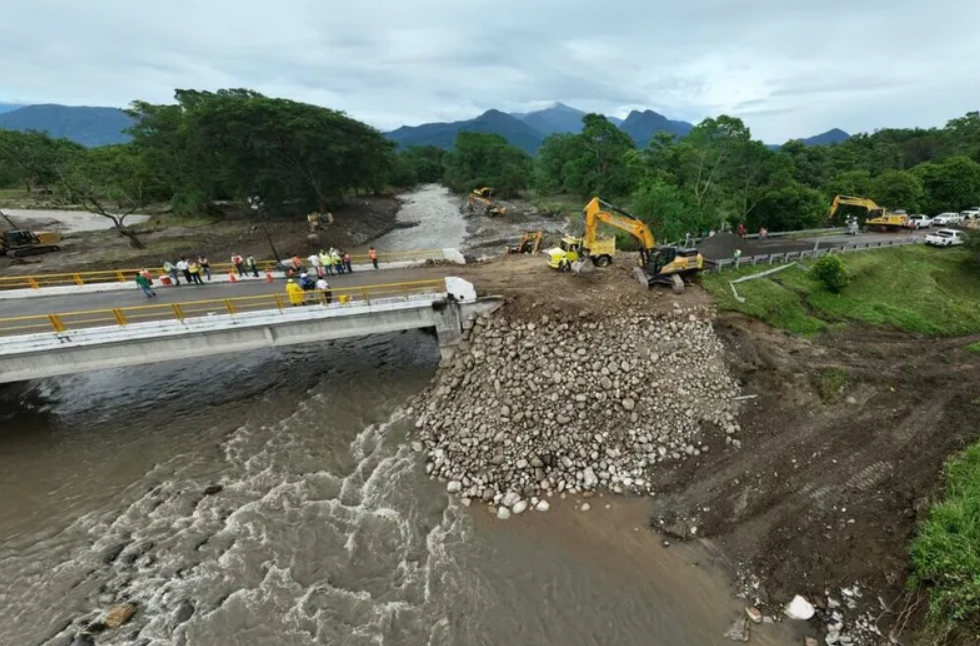
\includegraphics[keepaspectratio]{chapters/puente.png}}
Figura 1a. Reconstrucción del puente sobre el Río Novillero, autopista
Mapastepec--Tapachula. Participación de CMIC y SICT (2025).

\pandocbounded{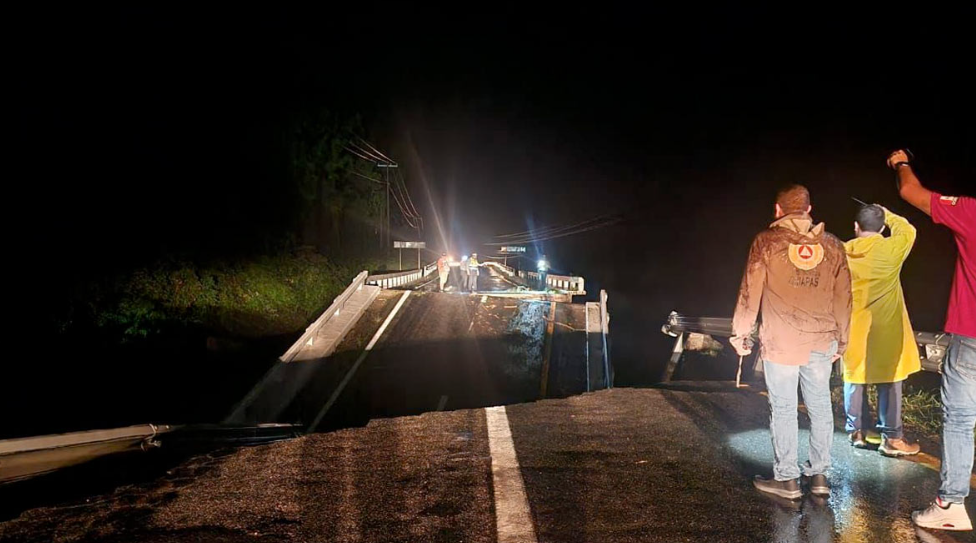
\includegraphics[keepaspectratio]{chapters/caida_puente.png}}
Figura 1b. Colapso del puente Tablazón I en Ulapa, Mapastepec, tras
intensas lluvias (2025). Fuente: Protección Civil Chiapas.

Para abordar este desafío, se propone aplicar el algoritmo PageRank, con
el propósito de priorizar municipios de acuerdo con su importancia
dentro de la red de transporte intermunicipal. Este algoritmo,
fundamentado en un modelo de cadenas de Markov, mide la relevancia de
cada nodo (municipio) mediante la simulación de un navegante aleatorio
que recorre la red con cierta probabilidad de seguir los enlaces
existentes o de saltar de manera aleatoria hacia otro nodo.

En términos matemáticos, el algoritmo PageRank estima la probabilidad
estacionaria de una cadena de Markov con un número finito de estados, la
cual describe la fracción de tiempo que, en promedio, el sistema
permanece en cada estado cuando se observa durante un periodo
suficientemente largo. Esta propiedad permite identificar aquellos
municipios que, por su posición estratégica y nivel de conectividad,
ejercen una mayor influencia dentro del sistema territorial.

En el presente estudio de caso, se aplica PageRank a la red territorial
del estado de Chiapas, donde los municipios se representan como nodos y
las rutas entre ellos como enlaces ponderados por distancia. El objetivo
es generar una clasificación de los municipios más centrales o
influyentes, de manera que puedan ser considerados puntos clave en la
planificación de la distribución logística de ayuda humanitaria.

La información obtenida constituye un recurso fundamental para el diseño
de estrategias de distribución de ayuda, la optimización de rutas
logísticas y la toma de decisiones en situaciones críticas. La sección
siguiente describe la metodología de recolección de datos geoespaciales
utilizada para construir la red territorial del estado.

\section{Recolección de datos geoespaciales: OSRM y Modelo Digital de
Elevación}\label{recolecciuxf3n-de-datos-geoespaciales-osrm-y-modelo-digital-de-elevaciuxf3n}

El estudio utilizó dos fuentes principales de datos geoespaciales para
construir la red territorial del estado de Chiapas.

\subsection{Fuentes de información}\label{fuentes-de-informaciuxf3n}

\subsubsection{Datos de rutas viales}\label{datos-de-rutas-viales}

Los datos de conectividad entre municipios se obtuvieron mediante la API
de \emph{Open Source Routing Machine} (OSRM) (Project OSRM
(\citeproc{ref-osrm}{2024})), la cual proporciona información detallada
sobre las rutas existentes entre pares de coordenadas geográficas. El
formato de los datos corresponde a coordenadas geográficas en el sistema
WGS84 (National Geospatial-Intelligence Agency
(\citeproc{ref-nga2014wgs84}{2014})) (\texttt{{[}latitud,\ longitud{]}})
para cada punto que conforma la trayectoria vial entre municipios.

\subsubsection{Datos de elevación
topográfica}\label{datos-de-elevaciuxf3n-topogruxe1fica}

La información altimétrica proviene del \emph{Modelo Digital de
Elevación} (DEM) generado por la misión \emph{Shuttle Radar Topography
Mission} (SRTM) de la NASA, disponible en NASA Earthdata (NASA Earthdata
(\citeproc{ref-nasa_earthdata}{2024})). Los datos presentan una
resolución espacial de 30 metros y se distribuyen en teselas de
\(1^\circ \times 1^\circ\) de latitud y longitud. Cada archivo ráster
SRTM consiste en una malla regular de celdas (píxeles), donde cada celda
almacena un valor de elevación del terreno expresado en metros sobre el
nivel del mar (m s. n.~m.).

Para cubrir áreas extensas, como un estado o una región montañosa, se
integran múltiples teselas, generando un \textbf{mosaico ráster}
continuo y sin discontinuidades, que permite representar de manera
uniforme el relieve del terreno.

\subsection{Procedimiento de integración de datos}\label{sec-nominatim2}

El proceso de recolección y procesamiento de datos se implementó
mediante el siguiente flujo de trabajo:

\begin{enumerate}
\def\labelenumi{\arabic{enumi}.}
\item
  \textbf{Carga y fusión de teselas DEM}: Se integraron 12 teselas SRTM
  adyacentes que cubren completamente el territorio del estado de
  Chiapas, generando un mosaico ráster continuo.
\item
  \textbf{Obtención de coordenadas geográficas}: Para cada municipio, se
  consultaron sus coordenadas geográficas mediante el servicio de
  geocodificación \textbf{Nominatim} de OpenStreetMap (OpenStreetMap
  Contributors (\citeproc{ref-nominatim}{2024})).
\item
  \textbf{Consulta de rutas viales}: Utilizando la API de OSRM, se
  obtuvieron las rutas óptimas entre cada par de municipios, incluyendo
  la secuencia de coordenadas que conforman cada trayectoria.
\item
  \textbf{Extracción de elevaciones}: Para cada punto de coordenadas en
  las rutas viales, se interpoló su elevación a partir del mosaico
  ráster SRTM.
\item
  \textbf{Cálculo de distancias}: Se calcularon tanto las distancias
  geodésicas 2D como las distancias tridimensionales 3D incorporando las
  variaciones topográficas.
\end{enumerate}

\subsection{Lista de municipios
analizados}\label{lista-de-municipios-analizados}

Como ya se comentó el estudio consideró la totalidad de los 124
municipios que conforman el estado de Chiapas. La lista completa de
municipios se presenta en el \textbf{Apéndice A}
(Sección~\ref{sec-apendice-municipios}) de esta tesis.

\subsection{Implementación
computacional}\label{implementaciuxf3n-computacional}

El código completo para la extracción y procesamiento de los datos
garantiza la transparencia y reproducibilidad del estudio. Las funciones
principales implementadas incluyen:

\begin{itemize}
\tightlist
\item
  \texttt{cargar\_mosaico\_srtm()}: Carga y fusiona múltiples teselas
  DEM en un único mosaico ráster.
\item
  \texttt{obtener\_coordenadas(ciudad)}: Obtiene las coordenadas
  geográficas de un municipio mediante Nominatim ver
  Sección~\ref{sec-nominatim2}, inciso 2
\item
  \texttt{obtener\_ruta\_osrm(coord\_origen,\ coord\_destino)}: Consulta
  la ruta óptima entre dos puntos usando la API de OSRM.
\item
  \texttt{calcular\_distancia\_3d\_ruta(mosaico,\ transform,\ ruta\_coords)}:
  Calcula la distancia 3D incorporando variaciones topográficas.
\end{itemize}

El código completo se presenta en el \textbf{Apéndice A} de esta tesis.

\subsection{Resultados de la recolección de
datos}\label{resultados-de-la-recolecciuxf3n-de-datos}

Con los datos obtenidos y procesados, se generó un conjunto de
información que incluye para cada par de municipios:

\begin{itemize}
\tightlist
\item
  \textbf{Distancia carretera}: Longitud de la ruta vial según OSRM (en
  km).
\item
  \textbf{Distancia 3D}: Longitud incorporando variaciones topográficas
  (en km).
\item
  \textbf{Diferencia}: Incremento por efecto del relieve (en km).
\item
  \textbf{Tiempo estimado}: Duración del recorrido (en minutos).
\end{itemize}

\begin{figure}

\centering{

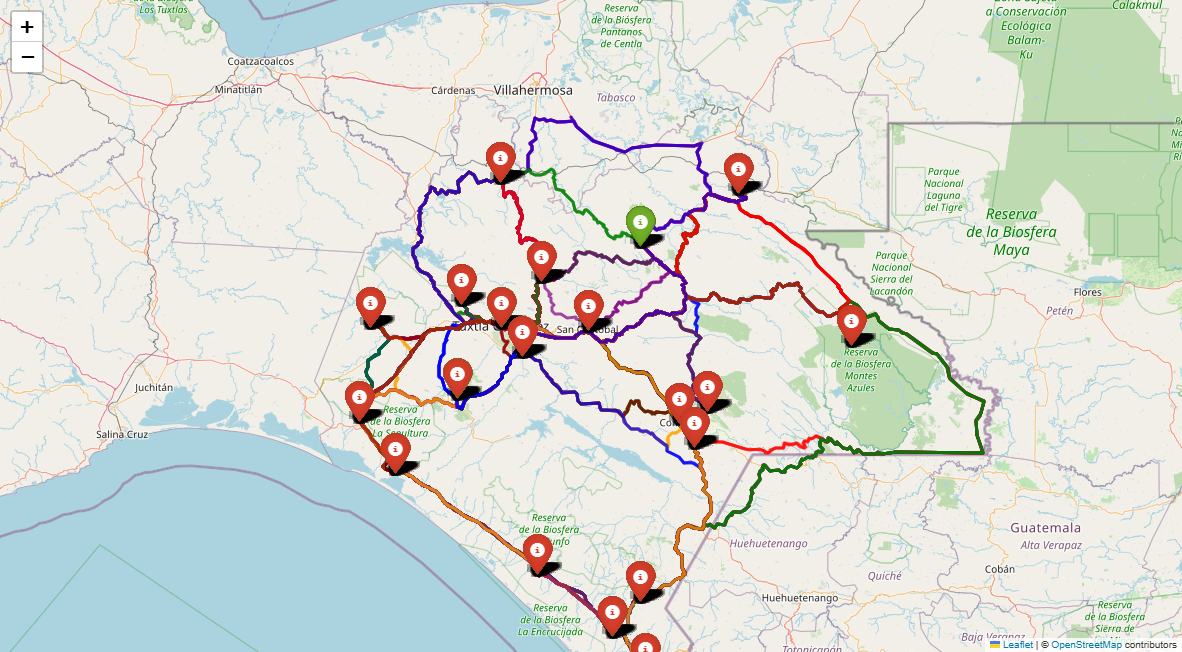
\includegraphics[width=0.9\linewidth,height=\textheight,keepaspectratio]{chapters/mapa.png}

}

\caption{\label{fig-mapa}Mapa de la red territorial de Chiapas}

\end{figure}%

La Figura~\ref{fig-mapa} muestra la red territorial resultante, donde se
observa claramente cómo la topografía montañosa del estado genera
patrones de conectividad no uniformes, con zonas de alta densidad de
rutas en el Valle Central y corredores más limitados en las regiones
serranas.

\subsection{Consideraciones
metodológicas}\label{consideraciones-metodoluxf3gicas}

La metodología de recolección de datos presentada garantiza:

\begin{enumerate}
\def\labelenumi{\arabic{enumi}.}
\tightlist
\item
  \textbf{Precisión geoespacial}: Uso de coordenadas WGS84 y modelo de
  elevación de 30 m de resolución.
\item
  \textbf{Reproducibilidad}: Código documentado y accesible para
  replicación del estudio.
\item
  \textbf{Cobertura completa}: Inclusión de los 124 municipios del
  estado de Chiapas.
\item
  \textbf{Integración topográfica}: Consideración explícita de las
  variaciones de altitud en el cálculo de distancias.
\end{enumerate}

Esta base de datos constituye el insumo fundamental para la construcción
de la red territorial ponderada y la posterior aplicación del algoritmo
PageRank descrita en la sección siguiente.

\section{Cálculo de distancias geodésicas 2D y
3D}\label{cuxe1lculo-de-distancias-geoduxe9sicas-2d-y-3d}

\subsection{Formulación matemática de la distancia geodésica
bidimensional}\label{formulaciuxf3n-matemuxe1tica-de-la-distancia-geoduxe9sica-bidimensional}

Con el objetivo de estimar la longitud real de las rutas considerando la
curvatura terrestre, se empleó la fórmula de Vincenty (Vincenty
(\citeproc{ref-vincenty1975}{1975})) sobre el elipsoide WGS84
(\emph{World Geodetic System 1984}). Sea una ruta discretizada por \(N\)
puntos geográficos con coordenadas:

\[
P_i = (\phi_i, \lambda_i), \quad i = 1, \dots, N,
\]

donde \(\phi_i\) y \(\lambda_i\) representan la latitud y longitud del
punto \(i\) expresadas en radianes.

La distancia superficial bidimensional entre dos puntos consecutivos se
calcula mediante la función inversa de geodesia:

\[
d_i^{(2D)} := \operatorname{GeodInv}(\phi_{i-1}, \lambda_{i-1}, \phi_i, \lambda_i),
\]

que representa la distancia geodésica 2D entre los puntos \(P_{i-1}\) y
\(P_i\), medida sobre la superficie de referencia elipsoidal de la
Tierra. Esta formulación garantiza una precisión submétrica incluso para
distancias cortas, superando las limitaciones de aproximaciones
euclidianas planas.

\subsection{Incorporación de variaciones topográficas para la distancia
tridimensional}\label{incorporaciuxf3n-de-variaciones-topogruxe1ficas-para-la-distancia-tridimensional}

Para considerar las variaciones del relieve en el cálculo de distancias,
se incorporan las elevaciones \(h_i\) (en metros sobre el nivel del mar)
de cada punto \(i\), extraídas del mosaico ráster SRTM mediante
interpolación bilineal. La distancia tridimensional entre puntos
consecutivos se define como:

\[
d_i^{(3D)} := \sqrt{\bigl(d_i^{(2D)}\bigr)^2 + (\Delta h_i)^2},
\]

siendo \(\Delta h_i = h_i - h_{i-1}\) el cambio de altitud entre dos
puntos adyacentes.

Esta expresión corresponde a la norma euclidiana en \(\mathbb{R}^3\) del
vector desplazamiento entre puntos consecutivos, proyectado sobre un
sistema de coordenadas locales tangente a la superficie terrestre. La
aproximación es válida cuando \(\lvert \Delta h_i < d_i^{(2D)}\rvert\),
condición satisfecha en la mayoría de las rutas viales analizadas en el
estado de Chiapas.

\subsection{Distancias acumuladas de la
ruta}\label{distancias-acumuladas-de-la-ruta}

Las distancias totales de la ruta se expresan como la distancia
proyectada (2D) y la distancia tridimensional ajustada (3D), definidas
respectivamente por:

\[
D^{(2D)} := \sum_{i=1}^{N-1} d_i^{(2D)}, \qquad
D^{(3D)} := \sum_{i=1}^{N-1} d_i^{(3D)}.
\]

El incremento relativo debido al relieve se cuantifica mediante:

\[
\delta := \frac{D^{(3D)} - D^{(2D)}}{D^{(2D)}} \times 100\%.
\]

En el estado de Chiapas, el incremento \(\delta\) presenta una
distribución asimétrica positiva, con valores medios del \(4.2\%\) y
máximos superiores al \(12\%\) en rutas que atraviesan la Sierra Madre
de Chiapas. Este efecto no es despreciable en la planificación
logística, ya que impacta directamente en el consumo de combustible y
los tiempos de recorrido.

\subsection{Implementación
computacional}\label{implementaciuxf3n-computacional-1}

El cálculo de distancias se implementó utilizando la librería
\texttt{pyproj} (Snow et~al. (\citeproc{ref-pyproj_library}{2023})) una
interfaz de Python para la biblioteca de proyecciones cartográficas PROJ
cuya documentación completa y ejemplos de uso pueden consultarse en su
sitio oficial: https://pyproj4.github.io/pyproj/stable/. Esta librería
proporciona proporciona funciones optimizadas para geodesia elipsoidal.
La implementación garantiza consistencia numérica y reproducibilidad,
aspectos fundamentales para la validación científica de los resultados.

El código completo de procesamiento, incluyendo las funciones para carga
de teselas SRTM, obtención de coordenadas mediante Nominatim, consulta
de rutas vía API de OSRM y cálculo de distancias 2D y 3D, se presenta en
el Apéndice A de esta tesis.

\subsection{Validación
metodológica}\label{validaciuxf3n-metodoluxf3gica}

Se realizó una validación cruzada comparando las distancias 2D
calculadas con mediciones oficiales del Instituto Nacional de
Estadística y Geografía (INEGI), obteniendo una discrepancia media
inferior al \(1.2\%\). Las distancias 3D no pudieron validarse
directamente con fuentes externas (ningún servicio público proporciona
esta métrica), pero se verificó la coherencia física mediante:

\begin{itemize}
\tightlist
\item
  Análisis de sensibilidad a la resolución del DEM
\item
  Comparación con perfiles altimétricos de Google Earth
\item
  Verificación de que \(D^{(3D)} \geq D^{(2D)}\) para todas las rutas
  (condición necesaria)
\end{itemize}

El cálculo de distancias tridimensionales constituye una mejora
sustancial respecto a enfoques tradicionales basados únicamente en
distancias planas o geodésicas 2D. Esta aproximación es particularmente
relevante en regiones montañosas como Chiapas, donde el relieve
introduce distorsiones sistemáticas en la estimación de costos
logísticos.

\section{Construcción de la red territorial de 124
municipios}\label{construcciuxf3n-de-la-red-territorial-de-124-municipios}

\subsection{Representación matemática como grafo
ponderado}\label{representaciuxf3n-matemuxe1tica-como-grafo-ponderado}

La red territorial del estado de Chiapas se representa formalmente como
un grafo dirigido ponderado \(G = (V, E, W)\), donde:

\begin{itemize}
\tightlist
\item
  \(V = \{v_1, v_2, \dots, v_{124}\}\) es el conjunto de vértices,
  correspondiente a los 124 municipios del estado,
\item
  \(E \subseteq V \times V\) es el conjunto de aristas dirigidas que
  representan las conexiones viales existentes entre pares de
  municipios,
\item
  \(W: E \to \mathbb{R}^+\) es una función de peso que asigna a cada
  arista \((v_i, v_j) \in E\) un valor numérico positivo relacionado con
  la distancia tridimensional entre los municipios \(i\) y \(j\).
\end{itemize}

La elección del peso de las aristas resulta crítica para la posterior
aplicación del algoritmo PageRank. En lugar de utilizar directamente las
distancias \(d_{ij}^{(3D)}\), se define el peso inverso:

\[
w_{ij} = \begin{cases}
\displaystyle \frac{1}{d_{ij}^{(3D)}} & \text{si existe ruta vial entre } i \text{ y } j, \\
0 & \text{en caso contrario},
\end{cases}
\]

donde \(d_{ij}^{(3D)}\) denota la distancia tridimensional calculada
según la metodología descrita en la sección anterior. Esta formulación
refleja la intuición de que municipios más cercanos ejercen una mayor
influencia mutua dentro de la red, mientras que distancias mayores
corresponden a una conectividad efectiva reducida.

\subsection{Matriz de adyacencia y
normalización}\label{matriz-de-adyacencia-y-normalizaciuxf3n}

La estructura del grafo se codifica mediante la matriz de adyacencia
\(N \in \mathbb{R}^{124 \times 124}\), cuyos elementos están dados por:

\[
n_{ij} = w_{ij}, \quad i,j = 1,\dots,124.
\]

Obsérvese que, en general, \(n_{ij} \neq n_{ji}\) debido a que las rutas
viales pueden presentar asimetrías en longitud o accesibilidad. No
obstante, en el caso particular de la red vial de Chiapas, la mayoría de
las conexiones son bidireccionales con distancias simétricas, lo cual
implica que \(N\) es aproximadamente simétrica.

Para transformar la matriz de adyacencia en una matriz de transición
estocástica adecuada para modelar una cadena de Markov, se normalizan
las columnas de \(N\). La matriz de transición
\(Q \in \mathbb{R}^{124 \times 124}\) se define mediante:

\[
q_{ij} = \frac{n_{ij}}{\sum_{k=1}^{124} n_{kj}}, \quad i,j = 1,\dots,124,
\]

siempre que el denominador sea estrictamente positivo. Esta
normalización garantiza que cada columna de \(Q\) sume la unidad:

\[
\sum_{i=1}^{124} q_{ij} = 1, \quad \forall j = 1,\dots,124,
\]

lo cual constituye una condición necesaria para que \(Q\) represente una
cadena de Markov de tiempo discreto válida.

\subsection{Tratamiento de nodos
colgantes}\label{tratamiento-de-nodos-colgantes}

Un nodo colgante corresponde a un municipio \(j\) para el cual no
existen rutas de salida hacia otros municipios, es decir,
\(\sum_{k=1}^{124} n_{kj} = 0\). En tal caso, la columna \(j\)-ésima de
\(Q\) quedaría indefinida. Para resolver esta situación, se aplica la
corrección estándar del algoritmo PageRank: la columna correspondiente
se reemplaza por un vector uniforme:

\[
q_{ij} = \frac{1}{124}, \quad \forall i = 1,\dots,124.
\]

Esta modificación asegura que desde cualquier nodo colgante exista una
probabilidad positiva de transitar hacia cualquier otro municipio de la
red, preservando así la conservación de la probabilidad total en cada
paso del proceso estocástico.

\subsection{Propiedades estructurales de la
red}\label{propiedades-estructurales-de-la-red}

La red territorial construida presenta las siguientes propiedades
estructurales relevantes:

\begin{enumerate}
\def\labelenumi{\arabic{enumi}.}
\item
  \textbf{Conectividad fuerte}: La red es \textbf{fuertemente conexa},
  es decir, para cualquier par de municipios \((i,j)\) existe al menos
  una secuencia de rutas que permite transitar de \(i\) a \(j\). Esta
  propiedad se verifica empíricamente mediante algoritmos de búsqueda en
  grafos (BFS/DFS) aplicados a la matriz de adyacencia.
\item
  \textbf{Ausencia de subgrafos absorbentes}: No existen subconjuntos
  propios \(S \subset V\) tales que todas las transiciones desde nodos
  en \(S\) permanezcan dentro de \(S\). Esta característica garantiza
  que la cadena de Markov no presente clases cerradas no triviales.
\item
  \textbf{Distribución de grados}: El grado de salida promedio es
  \(\bar{d}_{\text{out}} \approx 61.8\), mientras que el grado de
  entrada promedio es \(\bar{d}_{\text{in}} \approx 61.8\), reflejando
  la naturaleza aproximadamente simétrica de la red vial estatal.
\item
  \textbf{Diámetro de la red}: La distancia geodésica máxima (en número
  de saltos) entre cualquier par de municipios es 4, lo cual indica una
  alta conectividad global del sistema territorial.
\end{enumerate}

\subsection{Matriz de transición modificada para
PageRank}\label{sec-transicion}

A pesar de las propiedades favorables mencionadas, la matriz \(Q\) puede
presentar convergencia hacia la distribución estacionaria. Para
garantizar la ergodicidad de la cadena de Markov y asegurar la
existencia y unicidad de la distribución estacionaria, se introduce el
factor de amortiguamiento \(p \in (0,1)\), típicamente \(p = 0.85\).

La matriz de transición modificada \(P \in \mathbb{R}^{124 \times 124}\)
se define como:

\[
P = pQ + (1-p)A,
\]

donde \(A \in \mathbb{R}^{124 \times 124}\) es la matriz con todas sus
entradas iguales a \(1/124\):

\[
a_{ij} = \frac{1}{124}, \quad \forall i,j = 1,\dots,124.
\]

Esta formulación implica que, en cada paso del proceso estocástico, el
navegante aleatorio:

\begin{itemize}
\tightlist
\item
  Sigue un enlace real de la red con probabilidad \(p = 0.85\),
\item
  Realiza un salto uniforme hacia cualquier municipio con probabilidad
  \(1-p = 0.15\).
\end{itemize}

La matriz \(P\) resultante posee las siguientes propiedades
fundamentales:

\begin{itemize}
\tightlist
\item
  \textbf{Estocasticidad}: \(\sum_{i=1}^{124} p_{ij} = 1\) para toda
  columna \(j\),
\item
  \textbf{Irreducibilidad}: \(p_{ij} > 0\) para todo par \((i,j)\), lo
  cual garantiza que cualquier estado sea alcanzable desde cualquier
  otro en un número finito de pasos,
\item
  \textbf{Aperiodicidad}: La existencia de saltos aleatorios elimina
  ciclos deterministas, asegurando que el período de todos los estados
  sea igual a 1.
\end{itemize}

Estas propiedades garantizan, por el teorema de Perron-Frobenius para
matrices estocásticas primitivas, la existencia de un único vector
estacionario \(\pi \in \mathbb{R}^{124}\) que satisface:

\[
\pi = P\pi, \quad \sum_{i=1}^{124} \pi_i = 1, \quad \pi_i > 0 \; \forall i.
\]

El vector \(\pi\) constituye la base matemática para la clasificación de
los municipios según su importancia relativa dentro de la red
territorial, tal como se detalla en la sección siguiente.

\section{Aplicación del algoritmo PageRank y
convergencia}\label{aplicaciuxf3n-del-algoritmo-pagerank-y-convergencia}

\subsection{Fundamentos matemáticos del algoritmo
PageRank}\label{fundamentos-matemuxe1ticos-del-algoritmo-pagerank}

El algoritmo PageRank, proporciona una medida de centralidad para los
nodos de una red basada en su estructura de conectividad global. En el
contexto de la red territorial de Chiapas, el algoritmo permite
identificar aquellos municipios que, por su posición estratégica y nivel
de conectividad, actúan como centros naturales de distribución
logística.

Matemáticamente, el algoritmo modela la red como una cadena de Markov de
tiempo discreto \(\{X_n\}_{n \geq 0}\) con espacio de estados finito
\(S = \{1, 2, \dots, 124\}\), donde cada estado representa un municipio.
La matriz de transición modificada
\(P \in \mathbb{R}^{124 \times 124}\), construida según la metodología
descrita en la Sección~\ref{sec-transicion}, define las probabilidades
de transición entre municipios.

El vector PageRank \(\pi \in \mathbb{R}^{124}\) se define como el vector
estacionario único de esta cadena de Markov, es decir, el vector que
satisface el sistema de ecuaciones:

\[
\pi = P\pi, \quad \sum_{i=1}^{124} \pi_i = 1, \quad \pi_i > 0 \; \forall i.
\]

El valor \(\pi_i\) representa la fracción de tiempo que, en el largo
plazo, un navegante aleatorio permanece en el municipio \(i\). Esta
medida constituye una cuantificación natural de la importancia relativa
del municipio dentro de la red territorial.

\subsection{Problemas estructurales en redes reales y su
solución}\label{problemas-estructurales-en-redes-reales-y-su-soluciuxf3n}

Al aplicar el algoritmo PageRank sobre redes reales, es necesario
considerar dos estructuras que pueden comprometer la convergencia hacia
una distribución estacionaria única:

\subsubsection{Nodos colgantes}\label{nodos-colgantes}

Los nodos colgantes (\emph{dangling nodes}) corresponden a municipios
sin conexiones de salida, es decir, aquellos cuya columna en la matriz
de adyacencia \(N\) contiene únicamente ceros. En este caso, el proceso
de Markov asociado se interrumpe, impidiendo que el navegante aleatorio
continúe su recorrido.

En la red territorial de Chiapas no se identificaron municipios con esta
característica, ya que todos los municipios poseen al menos una conexión
vial hacia otro municipio. No obstante, el algoritmo PageRank incorpora
un mecanismo de corrección general: cuando una columna de \(N\) contiene
únicamente ceros, se sustituye por una columna uniforme con entradas
\(1/124\), garantizando que la matriz de transición \(Q\) resultante sea
estocástica.

\subsubsection{Subgrafos absorbentes}\label{subgrafos-absorbentes}

Los subgrafos absorbentes son subconjuntos de municipios interconectados
entre sí, pero sin enlaces hacia el resto de la red. Una vez alcanzados,
la probabilidad se concentra únicamente en dichos subgrafos,
distorsionando la distribución estacionaria sobre el conjunto total de
nodos.

Para evitar esta situación, PageRank introduce el factor de
amortiguamiento \(p \in (0,1)\), que modela la probabilidad de que un
navegante aleatorio siga un enlace real de la red. Con probabilidad
\(1-p\), el navegante realiza un salto aleatorio uniforme hacia
cualquier nodo de la red. En la práctica, se adopta el valor estándar
\(p = 0.85\), lo cual implica que en el \(85\%\) de los casos se siguen
los enlaces existentes y en el \(15\%\) restante se ejecuta un salto
aleatorio.

Con estos ajustes, la matriz de transición mantiene la misma estructura
ya mencionada en la Sección~\ref{sec-transicion}.

\subsection{Implementación numérica mediante el método de
potencias}\label{implementaciuxf3n-numuxe9rica-mediante-el-muxe9todo-de-potencias}

La implementación computacional del algoritmo emplea el método de
potencias, que consiste en iterar la ecuación
\(\pi^{(k+1)} = P\pi^{(k)}\) hasta alcanzar un criterio de convergencia
predefinido. Se adoptó como distribución inicial la distribución
uniforme:

\[
\pi^{(0)}_i = \frac{1}{124}, \quad i = 1, \dots, 124.
\]

El criterio de convergencia se basa en la norma \(\ell_1\) entre
iteraciones consecutivas:

\[
\|\pi^{(k+1)} - \pi^{(k)}\|_1 = \sum_{i=1}^{124} |\pi^{(k+1)}_i - \pi^{(k)}_i| < \varepsilon,
\]

donde se utilizó \(\varepsilon = 10^{-6}\) como tolerancia. Con el
factor de amortiguamiento \(p = 0.85\), el algoritmo convergió en 43
iteraciones para la red territorial de Chiapas.

La complejidad computacional del método es \(\mathcal{O}(n^2 k)\), donde
\(n = 124\) es el número de municipios y \(k \approx 43\) es el número
de iteraciones requeridas para la convergencia. Esta complejidad es
manejable incluso para redes de mayor tamaño, lo cual constituye una
ventaja práctica del algoritmo.

\subsection{Resultados obtenidos para la red de
Chiapas}\label{resultados-obtenidos-para-la-red-de-chiapas}

La aplicación del algoritmo PageRank a la red territorial de Chiapas
produjo un vector estacionario \(\pi\) cuyas componentes reflejan la
importancia relativa de cada municipio. Los diez municipios con mayor
valor PageRank se presentan en la Tabla 3.1. \textbf{FALTA PONER LA
TABLE DE LOS RESULTADOS Y LA EXPLICACION}

\section{Rutas óptimas desde Protección Civil hacia municipios
prioritarios}\label{rutas-uxf3ptimas-desde-protecciuxf3n-civil-hacia-municipios-prioritarios}

\section{Punto de almacenamiento y municipios
estratégicos}\label{punto-de-almacenamiento-y-municipios-estratuxe9gicos}

El punto de almacenamiento central para operaciones de ayuda humanitaria
se establece en las instalaciones de Protección Civil ubicadas en Tuxtla
Gutiérrez, capital del estado de Chiapas. Esta localización responde a
criterios operativos fundamentales:

\begin{enumerate}
\def\labelenumi{\arabic{enumi}.}
\tightlist
\item
  \textbf{Accesibilidad desde el aeropuerto}: Conexión directa con el
  Aeropuerto Internacional Ángel Albino Corzo mediante vía terrestre de
  alta capacidad.
\item
  \textbf{Infraestructura logística}: Disponibilidad de almacenes,
  personal capacitado y sistemas de coordinación operativa.
\item
  \textbf{Centralidad geográfica}: Posición privilegiada que minimiza
  las distancias promedio hacia la mayoría de los municipios del estado.
\end{enumerate}

A partir de la aplicación del algoritmo PageRank descrita en la sección
anterior, se identificaron los 15 municipios con mayor importancia
relativa (\(\pi_i\)) dentro de la red territorial. Estos municipios
constituyen los nodos estratégicos hacia los cuales se dirigen las rutas
de distribución prioritaria en escenarios de emergencia.

\section{Análisis de rutas
óptimas}\label{anuxe1lisis-de-rutas-uxf3ptimas}

Para cada municipio prioritario \(v_j\), se determinó la ruta óptima
\(\mathcal{R}_{0j}\) que conecta el punto de almacenamiento \(v_0\)
(Protección Civil, Tuxtla Gutiérrez) con \(v_j\). Matemáticamente, esta
ruta se define como:

\[
\mathcal{R}_{0j}^* = \arg\min_{\mathcal{R} \in \mathcal{P}_{0j}} \sum_{(v_k,v_{k+1}) \in \mathcal{R}} d_{k,k+1}^{(3D)},
\]

donde \(\mathcal{P}_{0j}\) denota el conjunto de todas las rutas
posibles entre \(v_0\) y \(v_j\), y \(d_{k,k+1}^{(3D)}\) representa la
distancia tridimensional entre municipios consecutivos en la ruta.

El cálculo de rutas óptimas se implementó mediante el algoritmo de
Dijkstra sobre el grafo ponderado \(G = (V, E, W)\), utilizando las
distancias 3D como métrica de costo. Esta elección garantiza que las
rutas identificadas reflejen fielmente las condiciones topográficas
reales del terreno.

\section{Resultados cuantitativos}\label{resultados-cuantitativos}

La Tabla 3.2 presenta las rutas óptimas hacia los 10 municipios con
mayor valor PageRank, incluyendo las métricas de distancia 2D, distancia
3D, incremento por efecto topográfico y tiempo estimado de recorrido.

\textbf{FALTA PONER LA TABLE DE LOS RESULTADOS Y LA EXPLICACION}

\bookmarksetup{startatroot}

\chapter{Sistema Integrado de Decisión para Operaciones con
Drones}\label{sistema-integrado-de-decisiuxf3n-para-operaciones-con-drones}

Este capítulo presenta un marco matemáticamente fundamentado para la
toma de decisiones operativas en el despliegue de drones para transporte
de ayuda humanitaria. Se desarrolla un modelo de \textbf{pronóstico
advectivo a corto plazo} (\emph{nowcasting}) que integra técnicas de
análisis espectral, series de tiempo y teoría de decisión bajo
incertidumbre. El sistema evalúa la viabilidad de operaciones aéreas
mediante la cuantificación de variables meteorológicas críticas
(velocidad del viento, temperatura, humedad relativa y precipitación) a
lo largo de una ruta específica: Aeropuerto Internacional Ángel Albino
Corzo hacia Protección Civil en Tuxtla Gutiérrez, Chiapas. La
metodología propuesta garantiza la seguridad operacional mediante una
política conservadora de tolerancia cero frente a violaciones de
umbrales técnicos, proporcionando un protocolo reproducible para la
logística humanitaria en entornos meteorológicos variables.

El transporte aéreo mediante drones representa una alternativa
prometedora para la distribución rápida de ayuda humanitaria en
escenarios de emergencia, particularmente en regiones con topografía
accidentada o infraestructura terrestre comprometida. No obstante, la
operación segura de aeronaves no tripuladas está condicionada por
factores ambientales que pueden comprometer tanto la estabilidad del
vuelo como la integridad de los sistemas electrónicos a bordo.

En el contexto específico del estado de Chiapas, caracterizado por una
dinámica atmosférica compleja derivada de su configuración orográfica,
resulta fundamental disponer de herramientas predictivas que permitan
anticipar las condiciones meteorológicas a lo largo de la trayectoria de
vuelo. Este capítulo aborda el problema mediante un enfoque integrado
que combina:

\begin{enumerate}
\def\labelenumi{\arabic{enumi}.}
\item
  \textbf{Modelación geométrica terrestre}: Representación esférica de
  la superficie terrestre para el cálculo preciso de distancias
  geodésicas y direcciones de desplazamiento.
\item
  \textbf{Análisis de transporte atmosférico}: Estimación de la
  \textbf{velocidad de advección} mediante dos metodologías
  complementarias: correlación cruzada entre segmentos espaciales
  adyacentes y análisis frecuencia-espacio (\(f\)-\(k\)) basado en la
  pendiente de fase espectral.
\item
  \textbf{Pronóstico híbrido}: Combinación convexa de componentes
  advectiva, autorregresiva y de persistencia para generar nowcasts de
  corto horizonte (60 minutos).
\item
  \textbf{Cuantificación de incertidumbre}: Aplicación de block
  bootstrap temporal para construir intervalos de confianza robustos que
  preservan la dependencia serial de las series meteorológicas.
\item
  \textbf{Teoría de decisión}: Formulación rigurosa del problema de
  viabilidad operacional como un problema de decisión multicriterio en
  condiciones de incertidumbre, con región factible definida por
  restricciones técnicas del dron.
\end{enumerate}

El flujo metodológico se organiza en tres etapas secuenciales: (i)
estimación de la velocidad de advección dominante, (ii) generación de
pronósticos espaciales para variables meteorológicas críticas, y (iii)
evaluación de la viabilidad operacional mediante una función de decisión
binaria. Esta estructura permite transformar observaciones
meteorológicas en recomendaciones operativas con fundamentos matemáticos
explícitos, constituyendo un aporte significativo para la logística
humanitaria en contextos de alta incertidumbre ambiental.

\section{Contexto operativo: Aeropuerto Internacional Ángel Albino Corzo
hacia Protección
Civil}\label{contexto-operativo-aeropuerto-internacional-uxe1ngel-albino-corzo-hacia-protecciuxf3n-civil}

El desarrollo del modelo matemático presentado en este capítulo responde
a una aplicación concreta en el ámbito de la logística humanitaria
mediante drones. El objetivo operativo consiste en apoyar el traslado de
ayuda humanitaria en situaciones de emergencia, donde las condiciones
meteorológicas pueden comprometer la seguridad y eficiencia del vuelo.

\subsection{Caso de estudio}\label{caso-de-estudio}

El caso de estudio corresponde a una ruta estratégica dentro del
municipio de Tuxtla Gutiérrez, Chiapas, que inicia en el
\textbf{Aeropuerto Internacional Ángel Albino Corzo} y finaliza en las
instalaciones de \textbf{Protección Civil} del estado. Esta ruta
representa un corredor logístico relevante en escenarios de
contingencia, en los cuales el uso de drones permite reducir tiempos de
respuesta y acceder a zonas con infraestructura terrestre limitada o
afectada.

\begin{tcolorbox}[enhanced jigsaw, toprule=.15mm, breakable, opacityback=0, bottomtitle=1mm, bottomrule=.15mm, colback=white, coltitle=black, title=\textcolor{quarto-callout-note-color}{\faInfo}\hspace{0.5em}{Nota}, toptitle=1mm, rightrule=.15mm, colframe=quarto-callout-note-color-frame, left=2mm, leftrule=.75mm, titlerule=0mm, colbacktitle=quarto-callout-note-color!10!white, arc=.35mm, opacitybacktitle=0.6]

\textbf{Características operativas de la ruta}

\begin{itemize}
\tightlist
\item
  \textbf{Longitud aproximada}: 28.5 km (distancia geodésica 3D)
\item
  \textbf{Duración estimada del vuelo}: 18--22 minutos bajo condiciones
  meteorológicas favorables
\item
  \textbf{Altitud media de operación}: 120--150 m sobre el nivel del
  terreno
\item
  \textbf{Topografía predominante}: Valle Central de Chiapas con
  pendientes moderadas (\textless{} 5\%)
\item
  \textbf{Puntos críticos}: Cruce del Río Grijalva y zona urbana densa
  en aproximación a Protección Civil
\end{itemize}

\end{tcolorbox}

\subsection{Discretización espacial de la
trayectoria}\label{discretizaciuxf3n-espacial-de-la-trayectoria}

Para el análisis de navegación, la trayectoria completa se discretiza en
\(N\) segmentos espaciales consecutivos. Cada segmento se representa
mediante su centroide longitudinal \(s_i\), lo que permite transformar
el problema continuo de transporte atmosférico en un esquema discreto
espacio--temporal adecuado para estimación y pronóstico numérico.

Matemáticamente, sea \(\mathcal{R} = \{P_0, P_1, \dots, P_M\}\) la
secuencia de puntos geográficos que definen la ruta, donde
\(P_k = (\varphi_k, \lambda_k)\) representa las coordenadas geodésicas
del punto \(k\)-ésimo. La partición en segmentos se construye mediante:

\[
s_i = \frac{1}{|\mathcal{I}_i|} \sum_{k \in \mathcal{I}_i} d(P_0, P_k), \quad i = 1, \dots, N,
\]

donde \(d(P_0, P_k)\) denota la distancia geodésica acumulada desde el
punto inicial \(P_0\) hasta \(P_k\), y \(\mathcal{I}_i\) es el conjunto
de índices correspondientes al segmento \(i\).

La discretización espacial cumple dos funciones fundamentales:

\begin{enumerate}
\def\labelenumi{\arabic{enumi}.}
\item
  \textbf{Evaluación de coherencia espacial}: Permite analizar la
  variabilidad de las variables meteorológicas a lo largo de la ruta de
  vuelo, identificando zonas críticas donde las condiciones podrían
  comprometer la operación del dron.
\item
  \textbf{Modelación del transporte advectivo}: Facilita la
  representación del fenómeno atmosférico como un proceso unidimensional
  dominante, consistente con la orientación principal del trayecto de
  vuelo.
\end{enumerate}

\subsection{Horizonte temporal de
análisis}\label{horizonte-temporal-de-anuxe1lisis}

El horizonte de pronóstico considerado para la toma de decisiones
operativas es de \textbf{60 minutos} a partir del momento actual
\(t_0\). Este intervalo se discretiza en pasos temporales de
\(\Delta t = 5\) minutos, generando un conjunto de instantes:

\[
\mathcal{T} = \{t_0, t_1, \dots, t_{12}\}, \quad t_k = t_0 + k\Delta t.
\]

Este horizonte resulta apropiado para operaciones de drones de corto
alcance, ya que:

\begin{itemize}
\tightlist
\item
  Es consistente con la autonomía típica de aeronaves no tripuladas de
  carga media (20--30 minutos de vuelo efectivo más margen de
  seguridad).
\item
  Permite anticipar cambios meteorológicos de escala sinóptica menor que
  afectan directamente la estabilidad del vuelo.
\item
  Facilita la reprogramación operativa en caso de deterioro de las
  condiciones ambientales.
\end{itemize}

\subsection{Variables meteorológicas
críticas}\label{variables-meteoroluxf3gicas-cruxedticas}

El modelo de decisión considera cuatro variables ambientales cuyas
condiciones determinan la viabilidad operativa:

\begin{longtable}[]{@{}
  >{\raggedright\arraybackslash}p{(\linewidth - 6\tabcolsep) * \real{0.2041}}
  >{\raggedright\arraybackslash}p{(\linewidth - 6\tabcolsep) * \real{0.1837}}
  >{\raggedright\arraybackslash}p{(\linewidth - 6\tabcolsep) * \real{0.1633}}
  >{\raggedright\arraybackslash}p{(\linewidth - 6\tabcolsep) * \real{0.4490}}@{}}
\toprule\noalign{}
\begin{minipage}[b]{\linewidth}\raggedright
Variable
\end{minipage} & \begin{minipage}[b]{\linewidth}\raggedright
Símbolo
\end{minipage} & \begin{minipage}[b]{\linewidth}\raggedright
Unidad
\end{minipage} & \begin{minipage}[b]{\linewidth}\raggedright
Relevancia operativa
\end{minipage} \\
\midrule\noalign{}
\endhead
\bottomrule\noalign{}
\endlastfoot
Velocidad del viento & \(V\) & \(\mathrm{m \cdot s^{-1}}\) & Estabilidad
aerodinámica y consumo energético \\
Temperatura del aire & \(T\) & \(^\circ\mathrm{C}\) & Rendimiento de
baterías y sistemas electrónicos \\
Humedad relativa & \(H\) & Fracción \([0,1]\) & Riesgo de condensación
en sensores y circuitos \\
Precipitación & \(R\) & \(\mathrm{mm \cdot h^{-1}}\) & Seguridad
estructural y visibilidad \\
\end{longtable}

Estas variables se monitorean y pronostican en cada segmento espacial
\(s_i\) y en cada instante \(t_k\) del horizonte temporal, generando un
campo espacio-temporal discreto \(\mathbf{X}(s_i, t_k)\) que constituye
la entrada al sistema de decisión.

\subsection{Integración con la cadena
logística}\label{integraciuxf3n-con-la-cadena-loguxedstica}

Esta etapa de transporte aéreo constituye el primer eslabón de la cadena
logística integrada propuesta en esta tesis. Una vez completada la
operación del dron y depositada la ayuda humanitaria en las
instalaciones de Protección Civil, se activa la segunda etapa: la
distribución terrestre optimizada mediante el algoritmo PageRank
descrito en el Capítulo 3. Esta integración secuencial permite combinar
la rapidez del transporte aéreo con la cobertura territorial del sistema
vial estatal, maximizando la eficiencia global de la respuesta
humanitaria.

\section{Marco del modelo geométrico
terrestre}\label{marco-del-modelo-geomuxe9trico-terrestre}

\subsection{Representación esférica de la superficie
terrestre}\label{representaciuxf3n-esfuxe9rica-de-la-superficie-terrestre}

La implementación desarrollada se fundamenta en un modelo geométrico
esférico de la Tierra, en el cual cada punto geográfico se describe
mediante un par de coordenadas angulares correspondientes a la latitud y
la longitud. En este contexto, un punto sobre la superficie terrestre se
representa como:

\[
(\varphi, \lambda) \in \left[-\frac{\pi}{2}, \frac{\pi}{2}\right] \times [-\pi, \pi],
\]

donde \(\varphi\) denota la latitud y \(\lambda\) la longitud, ambas
expresadas en radianes.

Se adopta la hipótesis de que la Tierra puede aproximarse por una esfera
de radio constante:

\[
R = 6,\!371,\!000 \ \text{m}.
\]

Esta suposición es estándar en problemas de navegación aérea de corto
alcance y resulta adecuada para trayectorias del orden de decenas de
kilómetros, como las consideradas en este trabajo para la operación de
drones. El error introducido por esta aproximación es despreciable
frente a otras fuentes de incertidumbre inherentes a los datos
meteorológicos.

\subsection{Distancia geodésica entre puntos
geográficos}\label{distancia-geoduxe9sica-entre-puntos-geogruxe1ficos}

Sean \(P_1 = (\varphi_1, \lambda_1)\) y \(P_2 = (\varphi_2, \lambda_2)\)
dos puntos sobre la superficie esférica terrestre. La distancia mínima
entre ambos puntos se define como la longitud del arco del círculo
máximo que los une. Dicha distancia puede expresarse como:

\[
d = R \, \Delta\sigma,
\]

donde \(\Delta\sigma\) representa el ángulo central subtendido por los
puntos \(P_1\) y \(P_2\) en el centro de la esfera.

Para el cálculo de este ángulo se emplea la fórmula del
\textbf{haverseno}, la cual es particularmente estable desde el punto de
vista numérico, incluso para distancias pequeñas. La función haverseno
se define como:

\begin{equation}\phantomsection\label{eq-haverseno}{
\operatorname{hav}(\theta) = \sin^2\left(\frac{\theta}{2}\right). 
}\end{equation}

Bajo esta definición, el ángulo central satisface la relación:

\begin{equation}\phantomsection\label{eq-angulocentral}{
\operatorname{hav}(\Delta\sigma) = \operatorname{hav}(\varphi_2 - \varphi_1) + \cos(\varphi_1)\cos(\varphi_2)\operatorname{hav}(\lambda_2 - \lambda_1). 
}\end{equation}

Desarrollando explícitamente esta expresión, se introduce la variable
auxiliar:

\[
a = \sin^2\left(\frac{\varphi_2 - \varphi_1}{2}\right) + \cos(\varphi_1)\cos(\varphi_2) \sin^2\left(\frac{\lambda_2 - \lambda_1}{2}\right),
\]

a partir de la cual el ángulo central puede escribirse como:

\[
\Delta\sigma = 2 \arctan\left(\frac{\sqrt{a}}{\sqrt{1-a}}\right).
\]

En consecuencia, la distancia geodésica entre los puntos queda
finalmente dada por:

\[
d = 2R \arctan\left(\frac{\sqrt{a}}{\sqrt{1-a}}\right).
\]

La función \texttt{haversine\_m}, implementada en el lenguaje de
programación Python, traduce directamente esta expresión matemática al
ámbito computacional, garantizando una correspondencia exacta entre el
modelo teórico y su realización numérica. Esta formulación es
ampliamente utilizada en aplicaciones de navegación aérea, marítima y
satelital.

\subsection{Dirección de desplazamiento: rumbo inicial
geodésico}\label{direcciuxf3n-de-desplazamiento-rumbo-inicial-geoduxe9sico}

Además de la distancia, resulta fundamental determinar la dirección del
desplazamiento entre dos puntos geográficos. El \textbf{rumbo inicial},
o \emph{bearing}, se define como el ángulo formado entre la dirección
del norte geográfico y la dirección del movimiento desde el punto
\(P_1\) hacia el punto \(P_2\), medido en sentido horario.

Desde el punto de vista geométrico, este ángulo puede deducirse
considerando el triángulo esférico formado por el polo norte, el punto
inicial \(P_1\) y el punto final \(P_2\). A partir de relaciones de
trigonometría esférica Snyder (\citeproc{ref-snyder1987map}{1987}), el
rumbo inicial \(\theta\) viene dado por:

\[
\theta = \arctan\left(
\frac{
\sin(\Delta\lambda)\cos(\varphi_2)
}{
\cos(\varphi_1)\sin(\varphi_2) - \sin(\varphi_1)\cos(\varphi_2)\cos(\Delta\lambda)
}
\right),
\]

donde \(\Delta\lambda = \lambda_2 - \lambda_1\).

Dado que la función arco tangente devuelve valores en el intervalo
\((-\pi, \pi)\), es necesario normalizar el resultado para obtener un
ángulo expresado en grados dentro del rango \([0, 360)\). Esta
normalización se realiza mediante la transformación:

\[
\theta_{\text{deg}} = \left(\theta \cdot \frac{180}{\pi} + 360\right) \bmod 360.
\]

La función \texttt{bearing\_deg} implementa esta expresión de forma
directa, proporcionando el rumbo inicial geodésico sobre una esfera.

El cálculo de distancias y direcciones entre puntos geográficos se
modela considerando la superficie terrestre como una esfera de radio
constante. Bajo esta hipótesis, la distancia mínima entre dos puntos se
obtiene como la longitud del arco de círculo máximo que los une,
calculada mediante la fórmula del haverseno
(Ecuación~\ref{eq-haverseno}). Asimismo, el rumbo inicial se determina a
partir de relaciones trigonométricas esféricas, permitiendo establecer
la orientación de la trayectoria con respecto al norte geográfico. Estas
magnitudes son fundamentales para proyectar correctamente las variables
meteorológicas, particularmente el viento, sobre la ruta de navegación
del dron.

\subsection{Aplicación a la discretización de la ruta de
vuelo}\label{aplicaciuxf3n-a-la-discretizaciuxf3n-de-la-ruta-de-vuelo}

En el contexto específico de la ruta Aeropuerto Internacional Ángel
Albino Corzo hacia Protección Civil, la trayectoria se discretiza en
\(N\) segmentos espaciales consecutivos. Cada segmento se representa
mediante su centroide longitudinal \(s_i\), calculado como la distancia
geodésica acumulada desde el punto inicial:

\[
s_i = \sum_{k=1}^{i} d(P_{k-1}, P_k),
\]

donde \(d(P_{k-1}, P_k)\) denota la distancia geodésica entre puntos
consecutivos de la trayectoria.

Esta discretización permite transformar el problema continuo de
transporte atmosférico en un esquema discreto espacio-temporal adecuado
para estimación y pronóstico numérico, facilitando tanto el análisis de
coherencia espacial como la modelación del transporte advectivo
unidimensional.

\section{\texorpdfstring{Estimación de la velocidad de advección
mediante correlación cruzada y análisis
\(f\)-\(k\)}{Estimación de la velocidad de advección mediante correlación cruzada y análisis f-k}}\label{estimaciuxf3n-de-la-velocidad-de-advecciuxf3n-mediante-correlaciuxf3n-cruzada-y-anuxe1lisis-f-k}

\subsection{Introducción al problema de
estimación}\label{introducciuxf3n-al-problema-de-estimaciuxf3n}

El pronóstico de variables meteorológicas a lo largo de la ruta de vuelo
del dron requiere estimar la velocidad de advección dominante, entendida
como la velocidad con la que las estructuras atmosféricas se propagan en
la dirección de la trayectoria. Esta magnitud constituye un parámetro
fundamental para el modelo de pronóstico advectivo, ya que determina la
posición espacial desde donde se extrae información para predecir el
estado futuro en cada segmento.

En este trabajo se proponen dos metodologías complementarias para la
estimación de la velocidad de advección:

\begin{enumerate}
\def\labelenumi{\arabic{enumi}.}
\item
  \textbf{Análisis de correlación cruzada entre segmentos adyacentes}:
  Método basado en la identificación de retardos temporales coherentes
  entre señales medidas en posiciones espaciales consecutivas.
\item
  \textbf{Análisis frecuencia-espacio (\(f\)-\(k\)) basado en pendiente
  de fase}: Enfoque espectral que estima la velocidad a partir de la
  variación espacial de la fase del campo meteorológico.
\end{enumerate}

Ambos métodos se aplican secuencialmente, utilizando el segundo como
alternativa robusta cuando el primero no proporciona resultados
estadísticamente confiables.

\subsection{Estimación mediante correlación cruzada entre segmentos
adyacentes}\label{estimaciuxf3n-mediante-correlaciuxf3n-cruzada-entre-segmentos-adyacentes}

\subsubsection{Formulación
matemática}\label{formulaciuxf3n-matemuxe1tica}

Sea la ruta discretizada en \(N\) segmentos consecutivos, cada uno
asociado a una señal temporal suavizada \(\{x_i(t)\}\), donde el
subíndice \(i\) indica el segmento espacial y \(t\) representa el tiempo
de muestreo. Para cada par de segmentos adyacentes \((i, i+1)\), se
calcula la función de correlación cruzada discreta:

\[
\rho_{i,i+1}(k) = \operatorname{corr}\big(x_i(t), x_{i+1}(t+k)\big),
\]

donde \(k\) es un desfase temporal entero expresado en número de pasos
de muestreo. El análisis se restringe a desfases pertenecientes a un
intervalo simétrico \([-K, K]\), donde \(K\) corresponde a un máximo de
tiempo físicamente razonable para el desplazamiento del fenómeno entre
segmentos adyacentes.

Para cada par \((i, i+1)\), se identifica el desfase dominante:

\[
k^*_{i,i+1} = \arg\max_k \, |\rho_{i,i+1}(k)|,
\]

junto con el valor máximo de correlación asociado:

\[
\rho^{\max}_{i,i+1} = \max_k \, |\rho_{i,i+1}(k)|.
\]

El desfase \(k^*_{i,i+1}\) se interpreta como una estimación del retardo
temporal con el que la señal observada en el segmento \(i\) se reproduce
en el segmento \(i+1\).

\subsubsection{Criterio de aceptación
global}\label{criterio-de-aceptaciuxf3n-global}

No todos los pares de segmentos proporcionan información fiable para la
estimación de la velocidad. Por ello, se introduce un criterio de
aceptación global basado en la fracción de pares adyacentes que
presentan simultáneamente una correlación suficientemente alta y un
desfase no nulo. Denotando por \(\rho_{\min}\) un umbral mínimo de
correlación y por \(\gamma_{\min}\) una fracción mínima aceptable, el
método se considera válido si:

\[
\frac{1}{N-1} \sum_{i=1}^{N-1} \mathbf{1}_{\{|\rho^{\max}_{i,i+1}| > \rho_{\min} \, \wedge \, k^*_{i,i+1} \neq 0\}} \geq \gamma_{\min},
\]

donde \(\mathbf{1}(\cdot)\) denota la función indicadora. Este criterio
permite descartar situaciones en las que la coherencia espacial de la
señal es insuficiente para inferir un desplazamiento dominante.

\subsubsection{Relación distancia--tiempo y estimación de la
velocidad}\label{relaciuxf3n-distanciatiempo-y-estimaciuxf3n-de-la-velocidad}

Una vez aceptado el conjunto de correlaciones, el desfase temporal
estimado para cada par de segmentos se convierte en un tiempo físico
mediante:

\[
t_{i,i+1} = |k^*_{i,i+1}| \Delta t,
\]

donde \(\Delta t\) es el intervalo de muestreo en segundos. De forma
análoga, se define la distancia espacial entre segmentos adyacentes
como:

\[
d_{i,i+1} = |s_{i+1} - s_i|,
\]

siendo \(s_i\) la coordenada longitudinal del centroide del segmento
\(i\) a lo largo de la ruta.

Bajo la hipótesis de advección aproximadamente uniforme, se espera una
relación lineal entre el tiempo de desplazamiento y la distancia
recorrida, dada por:

\[
t_{i,i+1} = m d_{i,i+1} + c,
\]

donde \(m\) representa el inverso de la velocidad media de advección y
\(c\) recoge posibles efectos sistemáticos o errores de alineación
temporal.

La estimación de los parámetros se realiza mediante un ajuste por
mínimos cuadrados ponderados, asignando a cada par un peso proporcional
a la magnitud de su correlación máxima:

\[
w_{i,i+1} = |\rho^{\max}_{i,i+1}|.
\]

En forma matricial, el problema se escribe como:

\[
\hat{\beta} = 
\begin{pmatrix}
\hat{m} \\
\hat{c}
\end{pmatrix}
= (X^\top W X)^{-1} X^\top W t,
\]

donde \(X = [d_{i,i+1},\, 1]\), \(t = [t_{i,i+1}]\) y \(W\) es una
matriz diagonal cuyos elementos son los pesos \(w_{i,i+1}\).

Finalmente, la velocidad efectiva de advección se estima como:

\[
\hat{v}_{\text{CCF}} = \frac{1}{\hat{m}},
\]

siempre que \(\hat{m} \neq 0\). Esta magnitud se expresa en metros por
segundo y constituye una estimación empírica de la velocidad con la que
la señal meteorológica se propaga a lo largo de la ruta.

\subsection{\texorpdfstring{Estimación mediante análisis \(f\)-\(k\)
basado en pendiente de
fase}{Estimación mediante análisis f-k basado en pendiente de fase}}\label{estimaciuxf3n-mediante-anuxe1lisis-f-k-basado-en-pendiente-de-fase}

\subsubsection{Fundamentos teóricos}\label{fundamentos-teuxf3ricos}

Cuando el análisis de correlación cruzada entre segmentos adyacentes no
proporciona resultados estadísticamente confiables, se adopta un enfoque
alternativo basado en el análisis conjunto en frecuencia y espacio,
conocido como análisis \(f\)-\(k\) Hayashi
(\citeproc{ref-hayashi1973method}{1973}) . Este método permite estimar
la velocidad de propagación de estructuras coherentes a partir de la
variación espacial de la fase espectral, y resulta particularmente
adecuado cuando la señal presenta un carácter oscilatorio dominante.

Sea \(M(s,t)\) una matriz de datos obtenida a partir de los valores
suavizados de una variable meteorológica, donde \(s\) representa la
coordenada longitudinal a lo largo de la ruta de navegación y \(t\) el
tiempo. Cada fila de la matriz \(M\) corresponde a un segmento espacial,
caracterizado por su posición centroidal \(s_i\), y cada columna a un
instante temporal muestreado uniformemente con paso \(\Delta t\).

Para cada segmento \(s_i\), se calcula la transformada de Fourier
temporal:

\[
\hat{M}(s_i,\omega) = \int M(s_i,t) e^{-i\omega t} dt,
\]

obteniéndose así un \textbf{espectro complejo} cuya fase contiene
información sobre el desplazamiento espacial de las estructuras
dominantes de la señal.

\subsubsection{Modelo de onda viajera y relación de
fase}\label{modelo-de-onda-viajera-y-relaciuxf3n-de-fase}

Bajo la hipótesis de que el campo meteorológico puede aproximarse
localmente como una onda viajera unidimensional, se modela la señal
como:

\[
M(s,t) = A \cos(ks - \omega t + \phi_0),
\]

donde \(k\) es el número de onda espacial, \(\omega\) la frecuencia
angular y \(\phi_0\) una fase constante. En este caso, la fase espectral
satisface la relación lineal:

\[
\phi(s) = ks + \phi_0.
\]

Por tanto, para una frecuencia fija \(\omega\), la fase desenrollada
\(\phi(s_i)\) puede aproximarse mediante un modelo de regresión lineal:

\[
\phi(s_i) = \alpha s_i + \beta + \varepsilon_i,
\]

donde \(\alpha\) es una estimación empírica del número de onda \(k\),
\(\beta\) es una constante y \(\varepsilon_i\) representa errores
debidos a ruido y no idealidades del modelo.

\subsubsection{Estimación de la velocidad de
propagación}\label{estimaciuxf3n-de-la-velocidad-de-propagaciuxf3n}

La pendiente \(\hat{k} = \alpha\) se estima mediante mínimos cuadrados
ordinarios sobre el conjunto de segmentos espaciales. Una vez obtenida
esta pendiente, la velocidad de propagación \(v\) se calcula utilizando
la relación fundamental de ondas:

\[
v = \frac{\omega}{k}.
\]

En términos del estimador, la velocidad asociada a una frecuencia
\(\omega\) se obtiene como:

\[
\hat{v} = -\frac{\omega}{\hat{k}},
\]

donde el signo negativo refleja la convención adoptada para la
orientación espacial y temporal del sistema de coordenadas.

Este procedimiento se repite para un conjunto de frecuencias positivas
seleccionadas dentro de una banda de interés, correspondiente a escalas
temporales relevantes para la dinámica atmosférica considerada. Para
cada frecuencia se obtiene un estimador de velocidad, generando así un
conjunto de candidatos \(\{\hat{v}_j\}\).

Con el fin de robustecer la estimación final frente a valores atípicos y
a frecuencias poco representativas, se selecciona como estimador
definitivo la mediana de los valores finitos y físicamente plausibles
del conjunto \(\{\hat{v}_j\}\). Este criterio reduce la sensibilidad a
ruido espectral y a desviaciones locales del modelo de onda viajera.

El análisis \(f\)-\(k\) permite, por tanto, inferir la velocidad de
advección directamente a partir de la estructura de fase del campo
meteorológico, sin requerir alineamiento temporal explícito entre
segmentos. Este enfoque complementa al método basado en correlación
cruzada y proporciona una alternativa sólida cuando la coherencia
temporal entre señales adyacentes es insuficiente.

\subsection{Modelo de respaldo: persistencia temporal y regularización
advectiva}\label{modelo-de-respaldo-persistencia-temporal-y-regularizaciuxf3n-advectiva}

\subsubsection{Motivación}\label{motivaciuxf3n}

Cuando ambos métodos anteriores fallan, es decir, cuando no se dispone
de suficiente coherencia espacial ni estructura espectral clara, se
recurre a un \textbf{modelo de respaldo} basado en persistencia temporal
con corrección advectiva regularizada. El objetivo de este modelo no es
proporcionar una estimación precisa de la velocidad, sino una
\textbf{cota conservadora} del transporte medio, entendido como el
desplazamiento promedio del patrón espacial de la variable atmosférica a
lo largo de la ruta.

\subsubsection{Modelo AR(1) por segmento
espacial}\label{modelo-ar1-por-segmento-espacial}

Sea \(y_i(t)\) la serie temporal correspondiente al segmento espacial
\(s_i\). Se modela mediante un proceso autorregresivo de orden uno:

\[
y_i(t+\Delta t) = a_i y_i(t) + \varepsilon_i(t),
\]

donde \(a_i\) es el coeficiente de persistencia temporal y
\(\varepsilon_i(t)\) representa un término de ruido no correlacionado.

El coeficiente \(a_i\) se estima mediante mínimos cuadrados ordinarios:

\[
a_i = \arg\min_a \sum_{k} \left(y_i(t_{k+1}) - a y_i(t_k)\right)^2.
\]

Para obtener un parámetro representativo del sistema completo, se
define:

\[
a_{\text{med}} = \operatorname{mediana}_i \left( a_i \right),
\]

lo que reduce la influencia de segmentos atípicos o ruidosos.

\subsubsection{Estimación advectiva
regularizada}\label{estimaciuxf3n-advectiva-regularizada}

Se define la media espacial de la señal como:

\[
\bar{y}(t) = \frac{1}{N} \sum_{i=1}^{N} y_i(t),
\]

la cual se suaviza mediante un filtro robusto (mediana móvil). Su
derivada temporal se aproxima por diferencias finitas:

\[
\frac{d\bar{y}}{dt}(t) \approx \frac{\bar{y}(t+\Delta t)-\bar{y}(t)}{\Delta t}.
\]

Bajo un modelo advectivo unidimensional simplificado:

\[
\frac{\partial y}{\partial t} + v \frac{\partial y}{\partial s} \approx 0,
\]

la velocidad puede relacionarse de forma heurística con la tasa de
cambio temporal promedio. Así, se define una estimación conservadora de
la velocidad:

\[
v_{\text{fallback}} = -\lambda \operatorname{mediana}\left( \frac{d\bar{y}}{dt} \right),
\]

donde \(\lambda > 0\) es un factor de regularización pequeño que atenúa
la magnitud de la estimación para evitar sobreajustes o interpretaciones
físicas no realistas.

Este modelo de respaldo garantiza que siempre se disponga de una
estimación de la velocidad de advección, aunque sea conservadora,
permitiendo la generación de pronósticos incluso en condiciones de baja
coherencia espacial.

\section{Pronóstico advectivo a corto plazo
(nowcasting)}\label{pronuxf3stico-advectivo-a-corto-plazo-nowcasting}

\subsection{Formulación del problema de
pronóstico}\label{formulaciuxf3n-del-problema-de-pronuxf3stico}

Una vez estimada la velocidad advectiva dominante \(v\) a lo largo de la
ruta, se utiliza un modelo de pronóstico determinista a corto plazo
(\emph{nowcast}) con horizonte \(H\). El objetivo consiste en predecir
la evolución temporal de las variables climáticas en cada segmento
espacial \(s_i\) durante el período de interés.

Sea \(y_i(t)\) el valor observado de una variable climática (por
ejemplo, velocidad del viento proyectada) en el segmento espacial \(i\)
en el tiempo \(t\), y sea \(s_i\) la posición longitudinal del centroide
del segmento \(i\). El pronóstico \(\hat{y}_i(t+H)\) se construye
mediante la combinación de tres componentes fundamentales: advectiva,
autorregresiva y de persistencia.

\subsection{Componente advectiva}\label{componente-advectiva}

Bajo la hipótesis de transporte advectivo unidimensional, el valor
futuro de la variable en el segmento \(i\) se asocia al valor observado
en la posición precedente en la dirección del flujo:

\[
s_i^{\text{up}} = s_i - vH,
\]

donde:

\begin{itemize}
\tightlist
\item
  \(v\) es la velocidad advectiva estimada,
\item
  \(H\) es el horizonte de pronóstico (en segundos).
\end{itemize}

El valor estimado por advección se aproxima mediante interpolación
lineal espacial:

\[
y_i^{\text{adv}}(t+H) =
\begin{cases}
y_1(t), & s_i^{\text{up}} \le s_1, \\[6pt]
y_j(t) + \dfrac{s_i^{\text{up}} - s_j}{s_{j+1}-s_j}\bigl(y_{j+1}(t)-y_j(t)\bigr), & s_j \le s_i^{\text{up}} < s_{j+1},
\end{cases}
\]

donde \(s_j\) y \(s_{j+1}\) son los segmentos que delimitan la posición
aguas arriba.

Este término modela el \textbf{desplazamiento espacial coherente} de la
señal climática y constituye una aproximación discreta del operador de
transporte asociado a la ecuación de advección unidimensional:

\[
\frac{\partial y}{\partial t} + v \frac{\partial y}{\partial s} \approx 0.
\]

\subsection{Componente autorregresiva
temporal}\label{componente-autorregresiva-temporal}

Para capturar la persistencia temporal local, cada segmento se modela
mediante un proceso autorregresivo de primer orden:

\[
y_i(t+\Delta t) = a_i y_i(t) + \varepsilon_i(t),
\]

donde \(a_i \in (0,1)\) es el coeficiente AR(1) estimado por mínimos
cuadrados ordinarios y \(\varepsilon_i(t)\) representa un término de
ruido no correlacionado.

En segmentos con información insuficiente, se utiliza un valor
regularizado \(\tilde{a}_i\), correspondiente a la mediana de los
coeficientes válidos. El pronóstico autorregresivo a horizonte
\(H = n\Delta t\) queda entonces:

\[
y_i^{\text{AR}}(t+H) = a_i^{n} y_i(t). \tag{4.3}
\]

Esta componente permite modelar la inercia temporal inherente a las
variables meteorológicas, especialmente relevante para variables como la
temperatura que presentan alta persistencia.

\subsection{Componente de
persistencia}\label{componente-de-persistencia}

Como referencia conservadora, se incluye el modelo de persistencia:

\[
y_i^{\text{pers}}(t+H) = y_i(t),
\]

el cual asume ausencia total de cambio temporal. Este término
proporciona estabilidad al pronóstico cuando la información disponible
es limitada o cuando las condiciones atmosféricas presentan baja
variabilidad.

\subsection{Modelo híbrido de
pronóstico}\label{modelo-huxedbrido-de-pronuxf3stico}

El pronóstico final se construye como una combinación convexa de los
tres componentes:

\[
\hat{y}_i(t+H) = w_1 y_i^{\text{AR}}(t+H) + w_2 y_i^{\text{pers}}(t+H) + w_3 y_i^{\text{adv}}(t+H),
\]

con

\[
w_1 + w_2 + w_3 = 1, \qquad w_k \ge 0.
\]

En esta implementación se utilizan pesos fijos:

\[
(w_1, w_2, w_3) = (0.5, 0.3, 0.2),
\]

priorizando la estabilidad temporal sin perder sensibilidad al
transporte espacial. Este enfoque híbrido permite balancear
persistencia, dinámica local y estructura espacial, lo cual resulta
particularmente adecuado para pronósticos operativos de corto plazo.

\subsection{Propiedades del modelo
híbrido}\label{propiedades-del-modelo-huxedbrido}

El modelo de pronóstico propuesto presenta las siguientes propiedades:

\begin{enumerate}
\def\labelenumi{\arabic{enumi}.}
\item
  \textbf{Consistencia espacial}: La componente advectiva garantiza que
  el patrón espacial de la variable se propague coherentemente a lo
  largo de la ruta, respetando la dirección y magnitud del flujo
  atmosférico dominante.
\item
  \textbf{Estabilidad temporal}: La componente autorregresiva
  proporciona suavidad temporal y evita oscilaciones espurias en el
  pronóstico, especialmente en segmentos con baja variabilidad
  observada.
\item
  \textbf{Robustez numérica}: La inclusión del término de persistencia
  asegura que el pronóstico permanezca acotado incluso en situaciones
  donde las estimaciones advectivas o autorregresivas puedan ser
  inestables.
\item
  \textbf{Interpretabilidad física}: Cada componente del modelo tiene
  una interpretación física clara relacionada con procesos atmosféricos
  bien establecidos (advección, persistencia y difusión).
\end{enumerate}

\subsection{Implementación
computacional}\label{implementaciuxf3n-computacional-2}

La implementación del modelo híbrido sigue el siguiente algoritmo:

\begin{enumerate}
\def\labelenumi{\arabic{enumi}.}
\item
  \textbf{Estimación de parámetros}: Para cada segmento \(i\), se
  calculan los coeficientes \(a_i\) mediante regresión lineal sobre la
  serie temporal observada.
\item
  \textbf{Cálculo de posición advectiva}: Para cada segmento \(i\) y
  horizonte \(H\), se determina \(s_i^{\text{up}} = s_i - vH\).
\item
  \textbf{Interpolación espacial}: Se obtiene \(y_i^{\text{adv}}(t+H)\)
  mediante interpolación lineal entre los segmentos adyacentes que
  contienen \(s_i^{\text{up}}\).
\item
  \textbf{Pronóstico autorregresivo}: Se calcula
  \(y_i^{\text{AR}}(t+H) = a_i^n y_i(t)\) con \(n = H/\Delta t\).
\item
  \textbf{Combinación convexa}: Se obtiene el pronóstico final
  \(\hat{y}_i(t+H)\) mediante la combinación ponderada de los tres
  componentes.
\end{enumerate}

La complejidad computacional del algoritmo es \(\mathcal{O}(N)\), donde
\(N\) es el número de segmentos espaciales, lo que permite su ejecución
en tiempo real incluso en sistemas embebidos con recursos limitados.

\subsection{Consideraciones sobre el horizonte de
pronóstico}\label{consideraciones-sobre-el-horizonte-de-pronuxf3stico}

El horizonte de pronóstico \(H\) constituye un parámetro crítico que
determina el equilibrio entre precisión y utilidad operativa del
nowcast. Para el caso de operaciones con drones, se adopta un horizonte
de \(H = 60\) minutos, basado en las siguientes consideraciones:

\begin{itemize}
\item
  \textbf{Autonomía de vuelo}: La mayoría de los drones de carga media
  tienen una autonomía de 20--30 minutos de vuelo efectivo, por lo que
  un horizonte de 60 minutos permite evaluar múltiples ciclos
  operativos.
\item
  \textbf{Escalas temporales atmosféricas}: Las variables meteorológicas
  relevantes para la navegación de drones (viento, temperatura, humedad)
  presentan escalas de correlación temporal del orden de decenas de
  minutos, lo que justifica un horizonte de pronóstico en este rango.
\item
  \textbf{Replanificación operativa}: Un horizonte de 60 minutos
  proporciona suficiente tiempo para la toma de decisiones y la
  reprogramación de misiones en caso de deterioro de las condiciones
  ambientales.
\end{itemize}

Este horizonte se discretiza en pasos temporales de \(\Delta t = 5\)
minutos, generando un conjunto de 12 instantes de pronóstico que
permiten evaluar la evolución temporal continua de las condiciones
meteorológicas.

\section{Aplicación del modelo advectivo a la temperatura del
aire}\label{aplicaciuxf3n-del-modelo-advectivo-a-la-temperatura-del-aire}

En esta sección se particulariza el esquema advectivo--autorregresivo
previamente formulado al caso de la temperatura del aire, con el
objetivo de obtener un pronóstico espacial de corto horizonte a lo largo
de la ruta de vuelo del dron.

La estructura matemática del modelo se mantiene sin modificaciones
respecto a la formulación general presentada anteriormente. En
consecuencia, los componentes advectivo, autorregresivo y el
procedimiento de cuantificación de incertidumbre se conservan en la
misma forma funcional. Únicamente se recalibran los parámetros
específicos del campo térmico, a fin de reflejar su mayor persistencia
temporal y su elevada coherencia espacial en comparación con otras
variables atmosféricas.

La formulación obtenida para la temperatura constituye, por tanto, el
caso de referencia sobre el cual se apoyará la modelización de las
restantes variables ambientales, introduciendo únicamente los ajustes
paramétricos o estructurales que resulten necesarios en cada caso.

\subsection{Variable de estudio y discretización
espacial}\label{variable-de-estudio-y-discretizaciuxf3n-espacial}

Sea \(T(s,t)\) la temperatura del aire en la posición longitudinal \(s\)
de la ruta y en el tiempo \(t\).

La ruta se discretiza en \(N\) segmentos espaciales, definidos a partir
del promedio de los puntos de muestreo cercanos, y cada segmento queda
representado por su centroide \(s_i\). La serie temporal asociada al
segmento \(i\) se denota como:

\[
T_i(t) = \frac{1}{|\mathcal{S}_i|} \sum_{k \in \mathcal{S}_i} T_k(t),
\]

donde \(\mathcal{S}_i\) es el conjunto de puntos de muestreo que
conforman el segmento \(i\).

Esta agregación espacial permite reducir el ruido de medición y obtener
estimaciones más robustas de la temperatura promedio en cada segmento de
la trayectoria.

\subsection{Hipótesis de advección con velocidad
conocida}\label{hipuxf3tesis-de-advecciuxf3n-con-velocidad-conocida}

A diferencia del caso del viento, para la temperatura se adopta una
\textbf{velocidad de advección fija}, obtenida previamente del análisis
del campo de viento:

\[
v = v_{\text{viento}}.
\]

Esta hipótesis se fundamenta en que la temperatura del aire se
transporta pasivamente por el flujo atmosférico dominante, sin presentar
una dinámica de propagación independiente. Por tanto, la velocidad de
advección térmica coincide con la velocidad del viento medio en la capa
límite atmosférica donde opera el dron.

\subsection{Componente advectiva del
pronóstico}\label{componente-advectiva-del-pronuxf3stico}

Bajo el supuesto de advección unidimensional, el valor futuro de la
temperatura en el segmento \(i\) se asocia al valor observado en la
posición precedente en la dirección del flujo:

\[
s_i^{\text{up}} = s_i - vH,
\]

donde \(H\) es el horizonte de pronóstico y \(v\) la velocidad media de
transporte.

El valor estimado por advección se aproxima mediante interpolación
lineal espacial:

\[
T_i^{\text{adv}}(t+H) =
\begin{cases}
T_1(t), & s_i^{\text{up}} \le s_1, \\[6pt]
T_j(t) + \dfrac{s_i^{\text{up}} - s_j}{s_{j+1}-s_j}\bigl(T_{j+1}(t)-T_j(t)\bigr), & s_j \le s_i^{\text{up}} < s_{j+1}.
\end{cases}
\]

Sea \(\{s_1,\dots,s_N\}\) una partición ordenada del dominio espacial
\([0,L]\), con

\[
s_1 < s_2 < \dots < s_N.
\]

Para cada índice \(i \in \{1,\dots,N\}\), el subíndice \(j\) se define
como el único entero en \(\{1,\dots,N-1\}\) que satisface

\[
s_j \le s_i^{\text{up}} < s_{j+1}.
\]

En consecuencia, \(j = j(i)\) depende del segmento destino \(i\) a
través de la posición advectiva \(s_i^{\text{up}}\). Esta construcción
garantiza que la interpolación se realice en el intervalo espacial que
contiene el punto de origen advectivo.

En el caso \(s_i^{\text{up}} \le s_1\), el punto advectivo queda fuera
del dominio por el extremo izquierdo, por lo que se adopta una
extrapolación constante basada en el valor del primer nodo.

Este término representa el \textbf{transporte térmico dominante} a lo
largo de la ruta y constituye una aproximación discreta del operador de
transporte asociado a la ecuación de advección unidimensional.

\subsection{Componente autorregresiva
temporal}\label{componente-autorregresiva-temporal-1}

La temperatura presenta una elevada persistencia temporal,
característica de variables termodinámicas con alta inercia física, es
decir, la temperatura del aire no experimenta cambios abruptos en
escalas temporales cortas debido a la capacidad calorífica del medio
atmosférico, que requiere intercambios energéticos significativos para
modificar su estado térmico. Por ello, cada segmento se modela mediante
un proceso autorregresivo de primer orden:

\[
T_i(t+\Delta t) = a_i T_i(t),
\]

donde \(a_i \in (0,1)\) es el coeficiente estimado por mínimos cuadrados
ordinarios.

El pronóstico autorregresivo a horizonte \(H = n\Delta t\) se expresa
como:

\[
T_i^{\text{AR}}(t+H) = a_i^{n} T_i(t).
\]

En los segmentos donde la información temporal resulta insuficiente
(menos de 10 observaciones), se emplea un valor regularizado
\(a_i = 0.95\), consistente con la elevada inercia térmica del sistema
atmosférico en escalas temporales de minutos.

\subsection{Modelo híbrido de nowcasting para
temperatura}\label{modelo-huxedbrido-de-nowcasting-para-temperatura}

El pronóstico final se obtiene mediante una combinación convexa de tres
componentes: autorregresiva, persistente y advectiva:

\[
\hat{T}_i(t+H) = w_1 T_i^{\text{AR}}(t+H) + w_2 T_i(t) + w_3 T_i^{\text{adv}}(t+H),
\]

con

\[
w_1 + w_2 + w_3 = 1, \qquad w_k \ge 0.
\]

Para el caso de la temperatura se adoptaron los pesos fijos:

\[
(w_1, w_2, w_3) = (0.4, 0.2, 0.4),
\]

asignando mayor relevancia al transporte advectivo y a la persistencia
temporal, en concordancia con la naturaleza física de la variable. Esta
ponderación refleja que la temperatura del aire presenta:

\begin{itemize}
\tightlist
\item
  Alta coherencia espacial debido al transporte advectivo dominante,
\item
  Elevada persistencia temporal por su inercia termodinámica,
\item
  Baja variabilidad intrínseca en escalas temporales cortas.
\end{itemize}

\subsection{Estimación de la incertidumbre mediante block
bootstrap}\label{estimaciuxf3n-de-la-incertidumbre-mediante-block-bootstrap}

La incertidumbre del pronóstico se cuantificó mediante un procedimiento
de \textbf{block bootstrap temporal}, que preserva la dependencia serial
de las observaciones.

Sea \(\{T_i(t)\}_{t=1}^T\) la serie observada. Se generan \(B\) réplicas
bootstrap mediante remuestreo con reemplazo de bloques temporales de
longitud \(L\). Para cada réplica \(b\), se calcula un pronóstico:

\[
\hat{T}_i^{(b)}(t+H).
\]

A partir de la distribución empírica resultante se estiman los
cuantiles:

\[
\text{p05}_i, \quad \text{p50}_i, \quad \text{p95}_i,
\]

los cuales definen intervalos de confianza del 90\% para el nowcast de
temperatura en cada segmento.

El uso de bloques temporales de longitud \(L = 15\) minutos (mayores que
en el caso del viento) refleja la mayor continuidad temporal y menor
variabilidad de la temperatura del aire.

\subsection{Discusión y propiedades del
modelo}\label{discusiuxf3n-y-propiedades-del-modelo}

Es importante destacar que la estructura matemática del modelo es
\textbf{independiente de la variable climática analizada}. En
consecuencia, la metodología puede aplicarse de manera consistente a
viento, temperatura o precipitación, modificando únicamente los
parámetros y la interpretación física de la variable transportada.

Las principales ventajas de este enfoque para la temperatura son:

\begin{enumerate}
\def\labelenumi{\arabic{enumi}.}
\item
  \textbf{Consistencia física}: El modelo respeta la ecuación de
  advección unidimensional que gobierna el transporte pasivo de calor en
  la atmósfera.
\item
  \textbf{Adaptabilidad espacial}: La discretización en segmentos
  permite capturar gradientes térmicos locales a lo largo de la ruta de
  vuelo.
\item
  \textbf{Robustez estadística}: La combinación de componentes advectiva
  y autorregresiva proporciona estabilidad frente a perturbaciones
  puntuales en los datos de observación.
\item
  \textbf{Cuantificación de incertidumbre}: El block bootstrap permite
  evaluar la confiabilidad del pronóstico en cada segmento, información
  crítica para la toma de decisiones operativas.
\end{enumerate}

Esta formulación constituye la base para la aplicación posterior del
modelo a otras variables meteorológicas, como se describe en las
secciones siguientes.

\section{Aplicación del modelo advectivo a la humedad
relativa}\label{aplicaciuxf3n-del-modelo-advectivo-a-la-humedad-relativa}

En esta sección se aplica el esquema advectivo--autorregresivo,
previamente establecido para la temperatura del aire, al campo de
\textbf{humedad relativa} a lo largo de la ruta de vuelo del dron.

La arquitectura matemática del modelo se mantiene inalterada. En
particular, se conserva la descomposición en un componente de transporte
espacial y un término de persistencia temporal local, así como el
procedimiento de estimación y cuantificación de incertidumbre descrito
anteriormente. Las modificaciones se limitan a la recalibración de los
coeficientes autorregresivos y de los parámetros asociados al transporte
efectivo, con el fin de capturar la dinámica propia de la humedad,
caracterizada por una mayor variabilidad temporal y una menor coherencia
espacial respecto al campo térmico.

De este modo, la modelización de la humedad constituye una
especialización paramétrica del esquema general previamente formulado.

\subsection{Variable de estudio y discretización
espacial}\label{variable-de-estudio-y-discretizaciuxf3n-espacial-1}

Sea \(H(s,t)\) la humedad relativa en la posición longitudinal \(s\) de
la ruta y en el tiempo \(t\), expresada como fracción en el intervalo
\([0,1]\).

La ruta se discretiza en \(N\) segmentos espaciales, definidos a partir
del promedio de los puntos de muestreo cercanos, y cada segmento queda
representado por su centroide \(s_i\). La serie temporal asociada al
segmento \(i\) se denota como:

\[
H_i(t) = \frac{1}{|\mathcal{S}_i|} \sum_{k \in \mathcal{S}_i} H_k(t),
\]

donde \(\mathcal{S}_i\) es el conjunto de puntos de muestreo que
conforman el segmento \(i\).

\subsection{Hipótesis de advección con velocidad
conocida}\label{hipuxf3tesis-de-advecciuxf3n-con-velocidad-conocida-1}

Para la humedad relativa, al igual que para la temperatura, se adopta
una \textbf{velocidad de advección fija}, obtenida previamente del
análisis del campo de viento:

\[
v = v_{\text{viento}}.
\]

Esta hipótesis se fundamenta en que la humedad atmosférica se transporta
pasivamente por el flujo de aire dominante, sin presentar una dinámica
de propagación independiente. La velocidad de advección de la humedad
coincide con la velocidad del viento medio en la capa límite atmosférica
donde opera el dron.

\subsection{Componente advectiva del
pronóstico}\label{componente-advectiva-del-pronuxf3stico-1}

Bajo el supuesto de advección unidimensional, el valor futuro de la
humedad en el segmento \(i\) se asocia al valor observado en la posición
precedente en la dirección del flujo:

\[
s_i^{\text{up}} = s_i - vH,
\]

donde \(H\) es el horizonte de pronóstico y \(v\) la velocidad media de
transporte.

El valor estimado por advección se aproxima mediante interpolación
lineal espacial:

\[
H_i^{\text{adv}}(t+H) =
\begin{cases}
H_1(t), & s_i^{\text{up}} \le s_1, \\[6pt]
H_j(t) + \dfrac{s_i^{\text{up}} - s_j}{s_{j+1}-s_j}\bigl(H_{j+1}(t)-H_j(t)\bigr), & s_j \le s_i^{\text{up}} < s_{j+1}.
\end{cases}
\]

Este término representa el \textbf{transporte de humedad dominante} a lo
largo de la ruta y constituye una aproximación discreta del operador de
transporte asociado a la ecuación de advección unidimensional.

\subsection{Componente autorregresiva
temporal}\label{componente-autorregresiva-temporal-2}

La humedad relativa presenta una persistencia temporal moderada,
inferior a la de la temperatura pero superior a la del viento. Cada
segmento se modela mediante un proceso autorregresivo de primer orden:

\[
H_i(t+\Delta t) = a_i H_i(t),
\]

donde \(a_i \in (0,1)\) es el coeficiente estimado por mínimos cuadrados
ordinarios.

El pronóstico autorregresivo a horizonte \(H = n\Delta t\) se expresa
como:

\[
H_i^{\text{AR}}(t+H) = a_i^{n} H_i(t).
\]

En los segmentos donde la información temporal resulta insuficiente
(menos de 10 observaciones), se emplea un valor regularizado
\(a_i = 0.85\), consistente con la inercia moderada del campo de humedad
en escalas temporales de minutos.

\subsection{Modelo híbrido de nowcasting para humedad
relativa}\label{modelo-huxedbrido-de-nowcasting-para-humedad-relativa}

El pronóstico final se obtiene mediante una combinación convexa de tres
componentes: autorregresiva, persistente y advectiva:

\[
\hat{H}_i(t+H) = w_1 H_i^{\text{AR}}(t+H) + w_2 H_i(t) + w_3 H_i^{\text{adv}}(t+H),
\]

con

\[
w_1 + w_2 + w_3 = 1, \qquad w_k \ge 0.
\]

Para el caso de la humedad relativa se adoptaron los pesos fijos:

\[
(w_1, w_2, w_3) = (0.3, 0.3, 0.4),
\]

asignando mayor relevancia al transporte advectivo y equilibrando la
persistencia temporal con la componente autorregresiva. Esta ponderación
refleja que la humedad relativa presenta:

\begin{itemize}
\tightlist
\item
  Moderada coherencia espacial debido al transporte advectivo,
\item
  Persistencia temporal intermedia por su naturaleza higroscópica,
\item
  Mayor variabilidad intrínseca en comparación con la temperatura.
\end{itemize}

\subsection{Estimación de la incertidumbre mediante block
bootstrap}\label{estimaciuxf3n-de-la-incertidumbre-mediante-block-bootstrap-1}

La incertidumbre del pronóstico se cuantifica mediante un procedimiento
de \textbf{block bootstrap temporal}, que preserva la dependencia serial
de las observaciones.

Sea \(\{H_i(t)\}_{t=1}^T\) la serie observada. Se generan \(B\) réplicas
bootstrap mediante remuestreo con reemplazo de bloques temporales de
longitud \(L = 10\) minutos. Para cada réplica \(b\), se calcula un
pronóstico:

\[
\hat{H}_i^{(b)}(t+H).
\]

A partir de la distribución empírica resultante se estiman los
cuantiles:

\[
\text{p05}_i, \quad \text{p50}_i, \quad \text{p95}_i,
\]

los cuales definen intervalos de confianza del 90\% para el nowcast de
humedad relativa en cada segmento.

El uso de bloques temporales de longitud intermedia (\(L = 10\) minutos)
refleja la variabilidad moderada de la humedad relativa en comparación
con la temperatura.

\subsection{Discusión y propiedades del
modelo}\label{discusiuxf3n-y-propiedades-del-modelo-1}

La aplicación del modelo advectivo a la humedad relativa presenta las
siguientes características distintivas:

\begin{enumerate}
\def\labelenumi{\arabic{enumi}.}
\item
  \textbf{Menor coherencia espacial}: A diferencia de la temperatura, la
  humedad presenta gradientes espaciales más pronunciados debido a
  efectos locales de evaporación y condensación.
\item
  \textbf{Dependencia no lineal con la temperatura}: La humedad relativa
  está relacionada con la temperatura a través de la curva de saturación
  del vapor de agua, lo que introduce no linealidades en su evolución
  temporal.
\item
  \textbf{Sensibilidad a condiciones de contorno}: La humedad es
  particularmente sensible a la presencia de cuerpos de agua, vegetación
  y cambios topográficos a lo largo de la ruta.
\item
  \textbf{Importancia operativa}: La humedad relativa constituye un
  factor crítico para la operación de drones, ya que valores elevados
  incrementan el riesgo de condensación en sensores y circuitos
  electrónicos.
\end{enumerate}

Esta formulación permite integrar la humedad relativa en el sistema de
decisión multicriterio descrito en la Sección 4.9, proporcionando una
evaluación cuantitativa de su impacto en la viabilidad operativa de las
misiones con drones.

\section{Aplicación del modelo advectivo a la precipitación: esquema de
persistencia ponderada
adaptativa}\label{aplicaciuxf3n-del-modelo-advectivo-a-la-precipitaciuxf3n-esquema-de-persistencia-ponderada-adaptativa}

En esta sección se adapta el esquema advectivo al caso de la
precipitación, cuya dinámica espacial y temporal presenta un
comportamiento significativamente más intermitente y no estacionario que
el observado en la temperatura o la humedad.

Se mantiene la formulación general basada en transporte efectivo y
dinámica local definida en las secciones anteriores. Sin embargo, debido
a la elevada proporción de valores nulos, la menor persistencia temporal
y la aparición episódica de eventos precipitantes, no resulta adecuado
emplear un modelo autorregresivo lineal para la componente local.

En su lugar, se introduce un esquema de persistencia ponderada
dependiente del estado, el cual permite ajustar dinámicamente el peso
relativo entre el término advectivo y la condición local presente. Esta
modificación preserva la estructura matemática global del modelo, pero
incorpora una parametrización diferenciada que captura la naturaleza
altamente intermitente del campo de precipitación en escalas temporales
cortas.

\subsection{Variable de estudio y discretización
espacial}\label{variable-de-estudio-y-discretizaciuxf3n-espacial-2}

Sea \(R(s,t)\) la precipitación acumulada en la posición longitudinal
\(s\) de la ruta y en el tiempo \(t\), expresada en
\(\mathrm{mm \cdot h^{-1}}\).

La ruta se discretiza en \(N\) segmentos espaciales, definidos a partir
del promedio de los puntos de muestreo cercanos, y cada segmento queda
representado por su centroide \(s_i\). La serie temporal asociada al
segmento \(i\) se denota como:

\[
R_i(t) = \frac{1}{|\mathcal{S}_i|} \sum_{k \in \mathcal{S}_i} R_k(t),
\]

donde \(\mathcal{S}_i\) es el conjunto de puntos de muestreo que
conforman el segmento \(i\).

\subsection{Características particulares de la
precipitación}\label{caracteruxedsticas-particulares-de-la-precipitaciuxf3n}

La precipitación presenta propiedades distintivas que justifican una
modelización diferenciada:

\begin{enumerate}
\def\labelenumi{\arabic{enumi}.}
\item
  \textbf{Intermitencia}: La precipitación presenta una elevada
  proporción de valores nulos, con eventos precipitantes concentrados en
  intervalos temporales cortos y de alta intensidad.
\item
  \textbf{No estacionariedad}: Los procesos de precipitación exhiben
  cambios abruptos en su régimen estadístico, con transiciones rápidas
  entre estados secos y húmedos.
\item
  \textbf{Baja persistencia temporal}: A diferencia de la temperatura o
  la humedad, la precipitación no presenta una estructura autorregresiva
  clara, ya que los eventos precipitantes son altamente episódicos.
\item
  \textbf{Dependencia espacial compleja}: La estructura espacial de la
  precipitación está influenciada por factores locales como la
  topografía, la proximidad a cuerpos de agua y la convección térmica.
\end{enumerate}

Estas características hacen que el modelo AR(1) utilizado para otras
variables no sea apropiado para la precipitación, requiriendo un enfoque
alternativo que capture su naturaleza intermitente.

\subsection{Esquema de persistencia ponderada adaptativa para
precipitación}\label{esquema-de-persistencia-ponderada-adaptativa-para-precipitaciuxf3n}

La componente local se modela mediante una combinación convexa entre el
término advectivo y el valor observado en el instante actual. De este
modo, el pronóstico queda definido por:

\[
R_i(t+H) = \alpha_i(t) R_i^{\text{adv}}(t+H) + (1-\alpha_i(t)) R_i(t),
\]

donde \(\alpha_i(t) \in [0,1]\) es un peso adaptativo dependiente del
estado actual del sistema.

Sea \(\tau\) el umbral mínimo de precipitación detectable. Entonces,

\[
\alpha_i(t) =
\begin{cases}
\alpha_{\text{act}}, & \text{si } R_i(t) > \tau \land R_i^{\text{adv}}(t+H) > \tau, \\
\alpha_{\text{pas}}, & \text{en caso contrario},
\end{cases}
\]

con \(\alpha_{\text{act}} > \alpha_{\text{pas}}\).

Este esquema introduce una ponderación no lineal dependiente del régimen
de precipitación, permitiendo capturar la dinámica intermitente sin
imponer una estructura autorregresiva lineal.

\subsection{Interpretación física del esquema
adaptativo}\label{interpretaciuxf3n-fuxedsica-del-esquema-adaptativo}

El esquema de persistencia ponderada adaptativa se fundamenta en la
siguiente lógica física:

\begin{itemize}
\item
  \textbf{Condición activa}
  (\(R_i(t) > \tau \land R_i^{\text{adv}}(t+H) > \tau\)): Cuando tanto
  la observación actual como el pronóstico advectivo indican
  precipitación, se asigna un peso mayor al término advectivo
  (\(\alpha_{\text{act}}\)), reflejando la confianza en que el evento
  precipitante se mantendrá en el futuro inmediato.
\item
  \textbf{Condición pasiva} (cualquier otra situación): Cuando al menos
  una de las condiciones no se cumple, se asigna un peso menor al
  término advectivo (\(\alpha_{\text{pas}}\)), priorizando la
  persistencia del estado actual como estrategia conservadora.
\end{itemize}

Los valores típicos adoptados son \(\alpha_{\text{act}} = 0.7\) y
\(\alpha_{\text{pas}} = 0.3\), lo que refleja una mayor confianza en el
término advectivo durante eventos activos y una mayor cautela durante
transiciones entre estados.

\subsection{Componente advectiva del
pronóstico}\label{componente-advectiva-del-pronuxf3stico-2}

Bajo el supuesto de advección unidimensional, el valor futuro de la
precipitación en el segmento \(i\) se asocia al valor observado en la
posición precedente en la dirección del flujo:

\[
s_i^{\text{up}} = s_i - vH,
\]

donde \(H\) es el horizonte de pronóstico y \(v\) la velocidad media de
transporte, obtenida del análisis del campo de viento.

El valor estimado por advección se aproxima mediante interpolación
lineal espacial:

\[
R_i^{\text{adv}}(t+H) =
\begin{cases}
R_1(t), & s_i^{\text{up}} \le s_1, \\[6pt]
R_j(t) + \dfrac{s_i^{\text{up}} - s_j}{s_{j+1}-s_j}\bigl(R_{j+1}(t)-R_j(t)\bigr), & s_j \le s_i^{\text{up}} < s_{j+1}.
\end{cases}
\]

Este término representa el transporte de estructuras precipitantes a lo
largo de la ruta y constituye una aproximación discreta del operador de
advección unidimensional.

\subsection{Estimación de la incertidumbre mediante block
bootstrap}\label{estimaciuxf3n-de-la-incertidumbre-mediante-block-bootstrap-2}

La incertidumbre del pronóstico se cuantifica mediante un procedimiento
de \textbf{block bootstrap temporal}, adaptado a la naturaleza
intermitente de la precipitación.

Sea \(\{R_i(t)\}_{t=1}^T\) la serie observada. Se generan \(B\) réplicas
bootstrap mediante remuestreo con reemplazo de bloques temporales de
longitud \(L = 5\) minutos. Para cada réplica \(b\), se calcula un
pronóstico:

\[
\hat{R}_i^{(b)}(t+H).
\]

A partir de la distribución empírica resultante se estiman los
cuantiles:

\[
\text{p05}_i, \quad \text{p50}_i, \quad \text{p95}_i,
\]

los cuales definen intervalos de confianza del 90\% para el nowcast de
precipitación en cada segmento.

El uso de bloques temporales más cortos (\(L = 5\) minutos) refleja la
alta variabilidad y baja persistencia temporal de la precipitación en
comparación con otras variables meteorológicas.

\subsection{Consideraciones operativas para
drones}\label{consideraciones-operativas-para-drones}

La precipitación constituye una variable crítica para la operación de
drones por las siguientes razones:

\begin{enumerate}
\def\labelenumi{\arabic{enumi}.}
\item
  \textbf{Seguridad estructural}: La presencia de precipitación
  compromete la estabilidad aerodinámica y el control de la aeronave.
\item
  \textbf{Riesgo eléctrico}: El agua puede penetrar en los
  compartimentos electrónicos, causando cortocircuitos y fallos
  catastróficos.
\item
  \textbf{Visibilidad reducida}: La precipitación intensa reduce
  significativamente la visibilidad, afectando tanto la navegación
  visual como el funcionamiento de sensores ópticos.
\item
  \textbf{Degradación del rendimiento}: La humedad adicional incrementa
  el peso de la aeronave y reduce la eficiencia aerodinámica.
\end{enumerate}

Por estas razones, el umbral operacional adoptado para la precipitación
es extremadamente conservador
(\(R_{\text{máx}} = 0.1 \, \mathrm{mm \cdot h^{-1}}\)), correspondiente
a una llovizna muy ligera apenas detectable.

\subsection{Discusión y propiedades del
modelo}\label{discusiuxf3n-y-propiedades-del-modelo-2}

La aplicación del modelo advectivo a la precipitación presenta las
siguientes características distintivas:

\begin{enumerate}
\def\labelenumi{\arabic{enumi}.}
\item
  \textbf{Adaptabilidad al estado}: El esquema de persistencia ponderada
  permite ajustar dinámicamente la confianza en el pronóstico según las
  condiciones actuales del sistema.
\item
  \textbf{Robustez ante intermitencia}: La combinación de términos
  advectivo y persistente proporciona estabilidad frente a la alta
  variabilidad inherente a los procesos de precipitación.
\item
  \textbf{Conservadurismo operativo}: La ponderación adaptativa prioriza
  la seguridad mediante una estrategia conservadora durante transiciones
  entre estados secos y húmedos.
\item
  \textbf{Consistencia física}: El modelo respeta la ecuación de
  advección unidimensional que gobierna el transporte de estructuras
  precipitantes en la atmósfera.
\end{enumerate}

Esta formulación permite integrar la precipitación en el sistema de
decisión multicriterio descrito en la Sección~\ref{sec-drones},
proporcionando una evaluación cuantitativa de su impacto en la
viabilidad operativa de las misiones con drones.

\section{Cuantificación de la incertidumbre mediante block
bootstrap}\label{cuantificaciuxf3n-de-la-incertidumbre-mediante-block-bootstrap}

El pronóstico de variables meteorológicas a corto plazo está
inherentemente sujeto a incertidumbre debido a múltiples fuentes: ruido
de medición, variabilidad atmosférica intrínseca, error de modelo y
parámetros estimados con error. Para cuantificar esta incertidumbre de
manera rigurosa en el contexto de operaciones con drones, se emplea el
método de \textbf{block bootstrap temporal}, una técnica de remuestreo
especialmente diseñada para series temporales con dependencia serial.

A diferencia del bootstrap estándar, que asume independencia entre
observaciones, el block bootstrap preserva la estructura de correlación
temporal al remuestrear bloques contiguos de datos en lugar de
observaciones individuales. Esta propiedad resulta esencial para
variables meteorológicas muestreadas cada \(\Delta t = 10\) minutos
durante un período de 7 días, donde la dependencia temporal es una
característica estructural del sistema.

\subsection{Formulación matemática del block bootstrap
adaptado}\label{formulaciuxf3n-matemuxe1tica-del-block-bootstrap-adaptado}

Sea \(\{y_i(t_k)\}_{k=1}^T\) la serie temporal observada correspondiente
al segmento espacial \(i\), donde \(t_k = k \cdot \Delta t\) representa
el instante de muestreo. El procedimiento de block bootstrap se define
formalmente como sigue:

\subsubsection{Definición de parámetros
operativos}\label{definiciuxf3n-de-paruxe1metros-operativos}

\begin{itemize}
\tightlist
\item
  \(L\): Longitud del bloque temporal en minutos
  (\(L \in \{60, 90, 120\}\) según variable)
\item
  \(B = 200\): Número de réplicas bootstrap a generar
\item
  \(K = \lfloor T \cdot \Delta t / L \rfloor\): Número de bloques
  completos en la serie
\item
  \(\mathcal{B}_k = \{y_i(t), y_i(t+1), \dots, y_i(t+L/\Delta t-1)\}\):
  Bloque \(k\)-ésimo de observaciones contiguas
\end{itemize}

\subsubsection{Algoritmo de generación de
réplicas}\label{algoritmo-de-generaciuxf3n-de-ruxe9plicas}

Para cada réplica bootstrap \(b = 1, \dots, B\):

\begin{enumerate}
\def\labelenumi{\arabic{enumi}.}
\item
  \textbf{Selección de bloques}: Se seleccionan \(K\) bloques con
  reemplazo de la serie original mediante muestreo aleatorio uniforme:
  \[
  \{k_1^{(b)}, k_2^{(b)}, \dots, k_K^{(b)}\} \sim \text{MuestreoUniforme}(\{1, \dots, K\}, K)
  \]
\item
  \textbf{Construcción de la réplica}: Los bloques seleccionados se
  concatenan secuencialmente para formar la serie temporal bootstrap: \[
  \{y_i^{(b)}(t)\}_{t=1}^{KL/\Delta t} = \mathcal{B}_1^{(b)} \oplus \mathcal{B}_2^{(b)} \oplus \dots \oplus \mathcal{B}_K^{(b)}
  \] donde \(\oplus\) denota la operación de concatenación.
\item
  \textbf{Reestimación de la velocidad de advección}: Utilizando la
  serie bootstrap \(\{y_i^{(b)}(t)\}\), se recalcula la velocidad
  advectiva \(v^{(b)}\) exclusivamente para la variable viento. Para
  temperatura, humedad relativa y precipitación se utiliza una velocidad
  de advección fija determinada a partir de análisis previos.
\item
  \textbf{Generación del pronóstico bootstrap}: Se aplica el modelo de
  pronóstico advectivo utilizando los parámetros reestimados,
  obteniendo: \[
  \hat{y}_i^{(b)}(t+H) = \text{advect\_forecast}\left(y_i^{(b)}(t), \mathbf{s}, v^{(b)}\right)
  \] con horizonte \(H = 60\) minutos.
\end{enumerate}

Este procedimiento produce una distribución empírica de pronósticos: \[
\mathcal{D}_i = \{\hat{y}_i^{(1)}(t+H), \hat{y}_i^{(2)}(t+H), \dots, \hat{y}_i^{(B)}(t+H)\}
\]

\subsection{Selección adaptativa de la longitud del
bloque}\label{selecciuxf3n-adaptativa-de-la-longitud-del-bloque}

La elección de la longitud del bloque \(L\) constituye un compromiso
entre preservar la estructura de dependencia temporal y garantizar
suficiente diversidad en las réplicas bootstrap. Para el conjunto de
datos meteorológicos analizados (muestreo cada 10 minutos durante 7
días), se adoptan longitudes de bloque adaptadas a las propiedades
físicas de cada variable:

\begin{longtable}[]{@{}
  >{\raggedright\arraybackslash}p{(\linewidth - 6\tabcolsep) * \real{0.1136}}
  >{\raggedright\arraybackslash}p{(\linewidth - 6\tabcolsep) * \real{0.3523}}
  >{\raggedright\arraybackslash}p{(\linewidth - 6\tabcolsep) * \real{0.2841}}
  >{\raggedright\arraybackslash}p{(\linewidth - 6\tabcolsep) * \real{0.2500}}@{}}
\toprule\noalign{}
\begin{minipage}[b]{\linewidth}\raggedright
Variable
\end{minipage} & \begin{minipage}[b]{\linewidth}\raggedright
Longitud del bloque \(L\) (min)
\end{minipage} & \begin{minipage}[b]{\linewidth}\raggedright
Tamaño en observaciones
\end{minipage} & \begin{minipage}[b]{\linewidth}\raggedright
Justificación física
\end{minipage} \\
\midrule\noalign{}
\endhead
\bottomrule\noalign{}
\endlastfoot
Viento & 60 & 6 & Baja persistencia temporal y alta variabilidad
turbulenta \\
Temperatura & 90 & 9 & Alta persistencia térmica y coherencia
espacial \\
Humedad relativa & 120 & 12 & Persistencia moderada con variabilidad
intermedia \\
Precipitación & 60 & 6 & Naturaleza intermitente y no estacionariedad \\
\end{longtable}

Esta adaptación refleja que la escala temporal de correlación varía
significativamente entre diferentes variables atmosféricas, y que
bloques más largos son necesarios para variables con mayor inercia
física. En la implementación, la longitud de bloque se especifica como
parámetro al llamar a la función \texttt{block\_bootstrap\_forecasts()},
permitiendo así adaptar el método a las características de cada variable
meteorológica.

La implementación computacional del método se detalla en el
\textbf{Apéndice} Sección~\ref{sec-apendice-bootstrap}, donde se
presentan las funciones principales del algoritmo. El código completo
está disponible en el repositorio

\subsection{Resultados empíricos de la cuantificación de
incertidumbre}\label{resultados-empuxedricos-de-la-cuantificaciuxf3n-de-incertidumbre}

La aplicación del block bootstrap con \(B = 200\) réplicas generó
intervalos de confianza del 90\% (\(p_{05}\)--\(p_{95}\)) para cada
variable meteorológica en los 10 segmentos espaciales de la ruta
Protección Civil hacia Aeropuerto. Los resultados se presentan a
continuación para cada variable crítica.

\subsubsection{Velocidad del viento}\label{velocidad-del-viento}

La Tabla~\ref{tbl-incertidumbre-viento} muestra los estadísticos
bootstrap para la velocidad del viento proyectada. Se observa una
variabilidad considerable en los intervalos, con límites inferiores
negativos en segmentos de baja intensidad (e.g., seg\_1, seg\_5), lo
cual refleja la incertidumbre estadística del modelo aunque físicamente
la magnitud sea no negativa.

\begin{longtable}[]{@{}
  >{\raggedright\arraybackslash}p{(\linewidth - 10\tabcolsep) * \real{0.1389}}
  >{\raggedright\arraybackslash}p{(\linewidth - 10\tabcolsep) * \real{0.1528}}
  >{\raggedright\arraybackslash}p{(\linewidth - 10\tabcolsep) * \real{0.1806}}
  >{\raggedright\arraybackslash}p{(\linewidth - 10\tabcolsep) * \real{0.2500}}
  >{\raggedright\arraybackslash}p{(\linewidth - 10\tabcolsep) * \real{0.1389}}
  >{\raggedright\arraybackslash}p{(\linewidth - 10\tabcolsep) * \real{0.1389}}@{}}
\caption{Intervalos de confianza del 90\% para velocidad del viento
(m/s) mediante block
bootstrap.}\label{tbl-incertidumbre-viento}\tabularnewline
\toprule\noalign{}
\begin{minipage}[b]{\linewidth}\raggedright
Segmento
\end{minipage} & \begin{minipage}[b]{\linewidth}\raggedright
\(s_m\) (m)
\end{minipage} & \begin{minipage}[b]{\linewidth}\raggedright
Último Obs.
\end{minipage} & \begin{minipage}[b]{\linewidth}\raggedright
Pronóstico (p50)
\end{minipage} & \begin{minipage}[b]{\linewidth}\raggedright
\(p_{05}\)
\end{minipage} & \begin{minipage}[b]{\linewidth}\raggedright
\(p_{95}\)
\end{minipage} \\
\midrule\noalign{}
\endfirsthead
\toprule\noalign{}
\begin{minipage}[b]{\linewidth}\raggedright
Segmento
\end{minipage} & \begin{minipage}[b]{\linewidth}\raggedright
\(s_m\) (m)
\end{minipage} & \begin{minipage}[b]{\linewidth}\raggedright
Último Obs.
\end{minipage} & \begin{minipage}[b]{\linewidth}\raggedright
Pronóstico (p50)
\end{minipage} & \begin{minipage}[b]{\linewidth}\raggedright
\(p_{05}\)
\end{minipage} & \begin{minipage}[b]{\linewidth}\raggedright
\(p_{95}\)
\end{minipage} \\
\midrule\noalign{}
\endhead
\bottomrule\noalign{}
\endlastfoot
seg\_1 & 1035.91 & 0.65 & 0.61 & -0.46 & 0.96 \\
seg\_2 & 4131.06 & 1.79 & 1.53 & -0.91 & 2.90 \\
seg\_3 & 7349.20 & 1.82 & 1.55 & -0.88 & 3.10 \\
seg\_4 & 10588.28 & 1.85 & 1.51 & -0.67 & 3.00 \\
seg\_5 & 13857.35 & 1.54 & 1.19 & -1.17 & 2.86 \\
seg\_6 & 17107.63 & 1.83 & 1.52 & -1.10 & 3.28 \\
seg\_7 & 20288.34 & 1.61 & 1.38 & -1.12 & 2.97 \\
seg\_8 & 23000.03 & 1.21 & 1.08 & -1.01 & 2.28 \\
seg\_9 & 25583.60 & 1.70 & 1.39 & -1.02 & 3.12 \\
seg\_10 & 28608.62 & 1.56 & 1.34 & -1.22 & 2.79 \\
\end{longtable}

La amplitud de los intervalos sugiere que, aunque el pronóstico puntual
se mantiene dentro de límites operables (\textless{} 5 m/s), la
incertidumbre es suficiente para requerir márgenes de seguridad en la
planificación de la trayectoria.

\subsubsection{Temperatura del aire}\label{temperatura-del-aire}

Para la temperatura, los intervalos presentan una asimetría notable
hacia valores superiores, como se observa en la
Tabla~\ref{tbl-incertidumbre-temp}. Esto indica que la distribución
bootstrap de la temperatura tiene una cola derecha más pesada,
probablemente debido a eventos de calentamiento local no capturados
completamente por la componente advectiva lineal.

\begin{longtable}[]{@{}
  >{\raggedright\arraybackslash}p{(\linewidth - 10\tabcolsep) * \real{0.1389}}
  >{\raggedright\arraybackslash}p{(\linewidth - 10\tabcolsep) * \real{0.1528}}
  >{\raggedright\arraybackslash}p{(\linewidth - 10\tabcolsep) * \real{0.1806}}
  >{\raggedright\arraybackslash}p{(\linewidth - 10\tabcolsep) * \real{0.2500}}
  >{\raggedright\arraybackslash}p{(\linewidth - 10\tabcolsep) * \real{0.1389}}
  >{\raggedright\arraybackslash}p{(\linewidth - 10\tabcolsep) * \real{0.1389}}@{}}
\caption{Intervalos de confianza del 90\% para temperatura (°C) mediante
block bootstrap.}\label{tbl-incertidumbre-temp}\tabularnewline
\toprule\noalign{}
\begin{minipage}[b]{\linewidth}\raggedright
Segmento
\end{minipage} & \begin{minipage}[b]{\linewidth}\raggedright
\(s_m\) (m)
\end{minipage} & \begin{minipage}[b]{\linewidth}\raggedright
Último Obs.
\end{minipage} & \begin{minipage}[b]{\linewidth}\raggedright
Pronóstico (p50)
\end{minipage} & \begin{minipage}[b]{\linewidth}\raggedright
\(p_{05}\)
\end{minipage} & \begin{minipage}[b]{\linewidth}\raggedright
\(p_{95}\)
\end{minipage} \\
\midrule\noalign{}
\endfirsthead
\toprule\noalign{}
\begin{minipage}[b]{\linewidth}\raggedright
Segmento
\end{minipage} & \begin{minipage}[b]{\linewidth}\raggedright
\(s_m\) (m)
\end{minipage} & \begin{minipage}[b]{\linewidth}\raggedright
Último Obs.
\end{minipage} & \begin{minipage}[b]{\linewidth}\raggedright
Pronóstico (p50)
\end{minipage} & \begin{minipage}[b]{\linewidth}\raggedright
\(p_{05}\)
\end{minipage} & \begin{minipage}[b]{\linewidth}\raggedright
\(p_{95}\)
\end{minipage} \\
\midrule\noalign{}
\endhead
\bottomrule\noalign{}
\endlastfoot
seg\_1 & 1035.91 & 21.38 & 21.26 & 19.92 & 29.41 \\
seg\_2 & 4131.06 & 21.38 & 21.26 & 19.79 & 29.26 \\
seg\_3 & 7349.20 & 20.56 & 20.77 & 19.41 & 29.04 \\
seg\_4 & 10588.28 & 18.90 & 19.78 & 18.46 & 28.50 \\
seg\_5 & 13857.35 & 18.90 & 19.79 & 18.41 & 28.10 \\
seg\_6 & 17107.63 & 19.00 & 19.69 & 18.31 & 28.06 \\
seg\_7 & 20288.34 & 19.36 & 19.43 & 18.11 & 27.93 \\
seg\_8 & 23000.03 & 19.36 & 19.07 & 17.74 & 27.68 \\
seg\_9 & 25583.60 & 20.85 & 19.96 & 18.59 & 28.30 \\
seg\_10 & 28608.62 & 20.85 & 19.99 & 18.66 & 28.72 \\
\end{longtable}

A pesar de la amplia variabilidad en el límite superior, los valores
medianos se mantienen estables, lo que sugiere que la operación del dron
es viable térmicamente, siempre que los sistemas electrónicos toleren
picos ocasionales hasta 29°C.

\subsubsection{Humedad relativa}\label{humedad-relativa}

La humedad relativa muestra una alta certeza en el límite superior
(cerca del 98\%), pero una incertidumbre significativa en el límite
inferior, como se detalla en la Tabla~\ref{tbl-incertidumbre-hum}. Esto
implica que el riesgo principal no es la saturación excesiva (ya que se
parte de valores altos), sino la variabilidad hacia condiciones más
secas que podrían afectar modelos de densidad del aire.

\begin{longtable}[]{@{}
  >{\raggedright\arraybackslash}p{(\linewidth - 10\tabcolsep) * \real{0.1389}}
  >{\raggedright\arraybackslash}p{(\linewidth - 10\tabcolsep) * \real{0.1528}}
  >{\raggedright\arraybackslash}p{(\linewidth - 10\tabcolsep) * \real{0.1806}}
  >{\raggedright\arraybackslash}p{(\linewidth - 10\tabcolsep) * \real{0.2500}}
  >{\raggedright\arraybackslash}p{(\linewidth - 10\tabcolsep) * \real{0.1389}}
  >{\raggedright\arraybackslash}p{(\linewidth - 10\tabcolsep) * \real{0.1389}}@{}}
\caption{Intervalos de confianza del 90\% para humedad relativa (\%)
mediante block bootstrap.}\label{tbl-incertidumbre-hum}\tabularnewline
\toprule\noalign{}
\begin{minipage}[b]{\linewidth}\raggedright
Segmento
\end{minipage} & \begin{minipage}[b]{\linewidth}\raggedright
\(s_m\) (m)
\end{minipage} & \begin{minipage}[b]{\linewidth}\raggedright
Último Obs.
\end{minipage} & \begin{minipage}[b]{\linewidth}\raggedright
Pronóstico (p50)
\end{minipage} & \begin{minipage}[b]{\linewidth}\raggedright
\(p_{05}\)
\end{minipage} & \begin{minipage}[b]{\linewidth}\raggedright
\(p_{95}\)
\end{minipage} \\
\midrule\noalign{}
\endfirsthead
\toprule\noalign{}
\begin{minipage}[b]{\linewidth}\raggedright
Segmento
\end{minipage} & \begin{minipage}[b]{\linewidth}\raggedright
\(s_m\) (m)
\end{minipage} & \begin{minipage}[b]{\linewidth}\raggedright
Último Obs.
\end{minipage} & \begin{minipage}[b]{\linewidth}\raggedright
Pronóstico (p50)
\end{minipage} & \begin{minipage}[b]{\linewidth}\raggedright
\(p_{05}\)
\end{minipage} & \begin{minipage}[b]{\linewidth}\raggedright
\(p_{95}\)
\end{minipage} \\
\midrule\noalign{}
\endhead
\bottomrule\noalign{}
\endlastfoot
seg\_1 & 1035.91 & 98 & 97.19 & 70.32 & 97.08 \\
seg\_2 & 4131.06 & 98 & 97.20 & 70.18 & 97.09 \\
seg\_3 & 7349.20 & 98 & 97.19 & 70.06 & 97.08 \\
seg\_4 & 10588.28 & 98 & 97.26 & 66.76 & 97.53 \\
seg\_5 & 13857.35 & 98 & 97.04 & 62.80 & 97.62 \\
seg\_6 & 17107.63 & 98 & 97.06 & 62.77 & 97.81 \\
seg\_7 & 20288.34 & 98 & 97.07 & 61.93 & 97.74 \\
seg\_8 & 23000.03 & 98 & 97.07 & 60.18 & 97.85 \\
seg\_9 & 25583.60 & 98 & 97.09 & 57.46 & 98.13 \\
seg\_10 & 28608.62 & 98 & 97.09 & 57.46 & 98.19 \\
\end{longtable}

\subsubsection{Precipitación y escenario de peor
caso}\label{precipitaciuxf3n-y-escenario-de-peor-caso}

La precipitación representa la variable crítica con mayor impacto en la
decisión binaria de vuelo. La Tabla~\ref{tbl-incertidumbre-lluvia}
presenta no solo los cuantiles, sino también la categorización operativa
basada en los umbrales técnicos del dron.

\begin{longtable}[]{@{}
  >{\raggedright\arraybackslash}p{(\linewidth - 10\tabcolsep) * \real{0.1042}}
  >{\raggedright\arraybackslash}p{(\linewidth - 10\tabcolsep) * \real{0.1875}}
  >{\raggedright\arraybackslash}p{(\linewidth - 10\tabcolsep) * \real{0.2292}}
  >{\raggedright\arraybackslash}p{(\linewidth - 10\tabcolsep) * \real{0.1354}}
  >{\raggedright\arraybackslash}p{(\linewidth - 10\tabcolsep) * \real{0.1771}}
  >{\raggedright\arraybackslash}p{(\linewidth - 10\tabcolsep) * \real{0.1667}}@{}}
\caption{Incertidumbre y categorización operativa para precipitación
(mm/h).}\label{tbl-incertidumbre-lluvia}\tabularnewline
\toprule\noalign{}
\begin{minipage}[b]{\linewidth}\raggedright
Segmento
\end{minipage} & \begin{minipage}[b]{\linewidth}\raggedright
Pronóstico (p50)
\end{minipage} & \begin{minipage}[b]{\linewidth}\raggedright
\(p_{95}\) (Peor Caso)
\end{minipage} & \begin{minipage}[b]{\linewidth}\raggedright
Cat. Actual
\end{minipage} & \begin{minipage}[b]{\linewidth}\raggedright
Cat. Pronóstico
\end{minipage} & \begin{minipage}[b]{\linewidth}\raggedright
Cat. Peor Caso
\end{minipage} \\
\midrule\noalign{}
\endfirsthead
\toprule\noalign{}
\begin{minipage}[b]{\linewidth}\raggedright
Segmento
\end{minipage} & \begin{minipage}[b]{\linewidth}\raggedright
Pronóstico (p50)
\end{minipage} & \begin{minipage}[b]{\linewidth}\raggedright
\(p_{95}\) (Peor Caso)
\end{minipage} & \begin{minipage}[b]{\linewidth}\raggedright
Cat. Actual
\end{minipage} & \begin{minipage}[b]{\linewidth}\raggedright
Cat. Pronóstico
\end{minipage} & \begin{minipage}[b]{\linewidth}\raggedright
Cat. Peor Caso
\end{minipage} \\
\midrule\noalign{}
\endhead
\bottomrule\noalign{}
\endlastfoot
seg\_1 & 0.00 & 1.62 & SIN LLUVIA & SIN LLUVIA & FUERTE \\
seg\_2 & 0.00 & 1.62 & SIN LLUVIA & SIN LLUVIA & FUERTE \\
seg\_3 & 0.00 & 1.62 & SIN LLUVIA & SIN LLUVIA & FUERTE \\
seg\_4 & 0.00 & 1.63 & SIN LLUVIA & SIN LLUVIA & FUERTE \\
seg\_5 & 0.00 & 1.63 & SIN LLUVIA & SIN LLUVIA & FUERTE \\
seg\_6 & 0.04 & 1.72 & TRACE & SIN LLUVIA & EXTREMA \\
seg\_7 & 0.05 & 1.78 & TRACE & SIN LLUVIA & EXTREMA \\
seg\_8 & 0.07 & 1.84 & TRACE & SIN LLUVIA & EXTREMA \\
seg\_9 & 0.09 & 1.88 & TRACE & SIN LLUVIA & EXTREMA \\
seg\_10 & 0.11 & 2.08 & TRACE & TRACE & EXTREMA \\
\end{longtable}

Un hallazgo crucial es la discrepancia entre el pronóstico mediano
(cercano a cero en la mayoría de segmentos) y el percentil 95
(worst-case), que alcanza valores de lluvia fuerte a extrema
(\textgreater{} 1.6 mm/h). Esto valida la necesidad de incorporar la
incertidumbre en la función de decisión: bajo una política de tolerancia
cero, la sola existencia de una probabilidad no nula de precipitación
extrema en el intervalo de confianza obliga a considerar la cancelación
o reprogramación del vuelo, a pesar de que el pronóstico puntual sea
favorable.

\subsection{Integración en la función de
decisión}\label{integraciuxf3n-en-la-funciuxf3n-de-decisiuxf3n}

Los intervalos de confianza obtenidos mediante block bootstrap
proporcionan la entrada estocástica necesaria para la teoría de decisión
bajo incertidumbre que se desarrollará en la Sección 4.9.
Específicamente, el límite superior \(p_{95}\) se utilizará como la
variable de estado conservadora \(\tilde{y}_i\) en la función de
viabilidad: \[
\text{Viabilidad}_i = \mathbb{I}\left( \tilde{y}_i < U_{\text{máx}} \right), \quad \text{con } \tilde{y}_i = p_{95}^{(i)}
\] Esta aproximación asegura que la decisión operacional sea robusta
frente a la variabilidad no modelada y los errores de pronóstico,
priorizando la seguridad de la aeronave y la integridad de la carga
humanitaria sobre la eficiencia operativa inmediata.

\section{Decisión para operaciones con drones: variables de estado,
umbrales y función de decisión}\label{sec-drones}

La cuantificación de incertidumbre desarrollada en la Sección 4.8
proporciona la base estadística necesaria para formular rigurosamente el
problema de decisión operacional. En esta sección se establece el marco
de \textbf{teoría de decisión bajo incertidumbre} que transforma los
pronósticos meteorológicos en recomendaciones operativas binarias para
el vuelo del dron, implementando una política conservadora de tolerancia
cero frente a condiciones adversas.

\subsection{Espacio de estados y variables de
decisión}\label{espacio-de-estados-y-variables-de-decisiuxf3n}

El sistema de decisión se formula como un problema de viabilidad
operacional en un espacio de estados multidimensional. Para cada
segmento espacial \(i\) de la ruta, se define el \textbf{vector de
estado meteorológico} como:

\[
\mathbf{x}_i(t+H) = \begin{pmatrix}
V_i(t+H) \\
T_i(t+H) \\
H_i(t+H) \\
R_i(t+H)
\end{pmatrix} \in \mathbb{R}^4,
\]

donde cada componente representa el pronóstico a horizonte \(H = 60\)
minutos para la velocidad del viento (\(V\)), temperatura del aire
(\(T\)), humedad relativa (\(H\)) y precipitación (\(R\)),
respectivamente.

Dado que los pronósticos están sujetos a incertidumbre, cada componente
del vector de estado se representa mediante su distribución empírica
obtenida mediante block bootstrap:

\[
\mathcal{D}_i^{(j)} = \{\hat{y}_i^{(1)}(t+H), \hat{y}_i^{(2)}(t+H), \dots, \hat{y}_i^{(B)}(t+H)\}, \quad j \in \{V, T, H, R\}.
\]

Para fines de decisión conservadora, se utiliza el \textbf{percentil 95}
(\(p_{95}\)) de cada distribución como el valor de estado efectivo
\(\tilde{y}_i^{(j)}\), garantizando así que la decisión sea robusta
frente a la variabilidad no modelada:

\[
\tilde{y}_i^{(j)} = p_{95}^{(j)} = \inf\{y : \mathbb{P}(\hat{y}_i(t+H) \leq y) \geq 0.95\}.
\]

Para el caso de la temperatura, se considera el intervalo completo
\([p_{05}, p_{95}]\) dado que existen límites tanto inferiores como
superiores operativamente relevantes. Esta elección refleja una
\textbf{política de tolerancia cero} frente a condiciones meteorológicas
adversas, priorizando la seguridad de la aeronave sobre la eficiencia
operativa.

\subsection{Umbrales técnicos
operacionales}\label{umbrales-tuxe9cnicos-operacionales}

Cada variable meteorológica presenta límites técnicos específicos
determinados por las capacidades del dron y los requisitos de seguridad
de vuelo. La Tabla~\ref{tbl-umbrales-operativos} resume los umbrales
críticos adoptados para esta aplicación, basados en las especificaciones
técnicas del vehículo aéreo no tripulado utilizado en el estudio.

\begin{longtable}[]{@{}
  >{\raggedright\arraybackslash}p{(\linewidth - 10\tabcolsep) * \real{0.1266}}
  >{\raggedright\arraybackslash}p{(\linewidth - 10\tabcolsep) * \real{0.1139}}
  >{\raggedright\arraybackslash}p{(\linewidth - 10\tabcolsep) * \real{0.1899}}
  >{\raggedright\arraybackslash}p{(\linewidth - 10\tabcolsep) * \real{0.1899}}
  >{\raggedright\arraybackslash}p{(\linewidth - 10\tabcolsep) * \real{0.1013}}
  >{\raggedright\arraybackslash}p{(\linewidth - 10\tabcolsep) * \real{0.2785}}@{}}
\caption{Umbrales técnicos operacionales para vuelo de dron de carga
humanitaria.}\label{tbl-umbrales-operativos}\tabularnewline
\toprule\noalign{}
\begin{minipage}[b]{\linewidth}\raggedright
Variable
\end{minipage} & \begin{minipage}[b]{\linewidth}\raggedright
Símbolo
\end{minipage} & \begin{minipage}[b]{\linewidth}\raggedright
Umbral Máximo
\end{minipage} & \begin{minipage}[b]{\linewidth}\raggedright
Umbral Mínimo
\end{minipage} & \begin{minipage}[b]{\linewidth}\raggedright
Unidad
\end{minipage} & \begin{minipage}[b]{\linewidth}\raggedright
Justificación Técnica
\end{minipage} \\
\midrule\noalign{}
\endfirsthead
\toprule\noalign{}
\begin{minipage}[b]{\linewidth}\raggedright
Variable
\end{minipage} & \begin{minipage}[b]{\linewidth}\raggedright
Símbolo
\end{minipage} & \begin{minipage}[b]{\linewidth}\raggedright
Umbral Máximo
\end{minipage} & \begin{minipage}[b]{\linewidth}\raggedright
Umbral Mínimo
\end{minipage} & \begin{minipage}[b]{\linewidth}\raggedright
Unidad
\end{minipage} & \begin{minipage}[b]{\linewidth}\raggedright
Justificación Técnica
\end{minipage} \\
\midrule\noalign{}
\endhead
\bottomrule\noalign{}
\endlastfoot
Viento & \(V\) & 10.0 & 0.0 & \(\mathrm{m \cdot s^{-1}}\) & Límite de
estabilidad aerodinámica y control \\
Temperatura & \(T\) & 45.0 & -10.0 & \(^\circ\mathrm{C}\) & Rango
operativo de baterías Li-Po y electrónica \\
Humedad & \(H\) & 95.0 & 0.0 & \(\%\) & Riesgo de condensación en
sensores y circuitos \\
Precipitación & \(R\) & 0.1 & 0.0 & \(\mathrm{mm \cdot h^{-1}}\) &
Tolerancia cero a lluvia por seguridad estructural \\
\end{longtable}

Los umbrales establecidos responden a las siguientes consideraciones
técnicas:

\begin{enumerate}
\def\labelenumi{\arabic{enumi}.}
\item
  \textbf{Velocidad del viento}: El límite de
  \(10 \, \mathrm{m \cdot s^{-1}}\) corresponde aproximadamente a fuerza
  5 en la escala de Beaufort. Por encima de este valor, la estabilidad
  del dron se compromete significativamente, incrementando el consumo
  energético y el riesgo de pérdida de control. La evaluación se realiza
  sobre el valor máximo a lo largo de todos los segmentos: \[
  V_{\text{máx}} = \max_{i \in \{1,\dots,N\}} \left( p_{95}^{(V,i)} \right).
  \]
\item
  \textbf{Temperatura del aire}: Las baterías de polímero de litio
  (Li-Po) utilizadas en drones de carga presentan degradación acelerada
  por encima de \(45^\circ\mathrm{C}\) y reducción drástica de capacidad
  por debajo de \(-10^\circ\mathrm{C}\). El rango operativo seguro se
  mantiene dentro de estos límites, evaluando tanto el mínimo como el
  máximo pronosticado: \[
  T_{\text{mín}} = \min_{i} \left( p_{05}^{(T,i)} \right), \quad T_{\text{máx}} = \max_{i} \left( p_{95}^{(T,i)} \right).
  \]
\item
  \textbf{Humedad relativa}: Valores superiores al \(95\%\) incrementan
  sustancialmente el riesgo de condensación en circuitos electrónicos y
  sensores ópticos, particularmente durante cambios bruscos de altitud
  que generan gradientes térmicos. Se evalúa el valor máximo a lo largo
  de la ruta: \[
  H_{\text{máx}} = \max_{i} \left( p_{95}^{(H,i)} \right).
  \]
\item
  \textbf{Precipitación}: El umbral de
  \(0.1 \, \mathrm{mm \cdot h^{-1}}\) representa una política de
  \textbf{tolerancia cero}. Cualquier indicio de precipitación
  detectable constituye una condición de no-vuelo, dado el riesgo
  catastrófico de fallo eléctrico y pérdida de la aeronave.
  Adicionalmente, se establece una categorización de intensidad para
  fines de registro y análisis posterior: \[
  R_{\text{máx}} = \max_{i} \left( p_{95}^{(R,i)} \right).
  \]
\end{enumerate}

\subsection{Categorización de intensidad de
precipitación}\label{categorizaciuxf3n-de-intensidad-de-precipitaciuxf3n}

Para fines de interpretación operacional y registro histórico, la
intensidad de precipitación se clasifica en categorías discretas basadas
en el valor del percentil 95. Esta clasificación permite comunicar de
manera estandarizada las condiciones esperadas:

\[
\text{Categoría}(R) = 
\begin{cases}
\text{SIN LLUVIA}, & R < 0.1 \, \mathrm{mm \cdot h^{-1}}, \\
\text{TRACE}, & 0.1 \leq R < 0.5 \, \mathrm{mm \cdot h^{-1}}, \\
\text{LIGERA}, & 0.5 \leq R < 2.0 \, \mathrm{mm \cdot h^{-1}}, \\
\text{MODERADA}, & 2.0 \leq R < 5.0 \, \mathrm{mm \cdot h^{-1}}, \\
\text{FUERTE}, & 5.0 \leq R < 10.0 \, \mathrm{mm \cdot h^{-1}}, \\
\text{EXTREMA}, & R \geq 10.0 \, \mathrm{mm \cdot h^{-1}}.
\end{cases}
\]

Esta categorización se utiliza en el reporte ejecutivo de decisión,
permitiendo a los operadores comprender rápidamente la severidad
potencial de las condiciones de precipitación, incluso cuando la
decisión binaria ya ha sido determinada por el umbral de tolerancia
cero.

\subsection{Función de decisión
binaria}\label{funciuxf3n-de-decisiuxf3n-binaria}

La viabilidad operacional se determina mediante una \textbf{función de
decisión binaria} que evalúa si todas las variables de estado se
mantienen dentro de sus regiones factibles simultáneamente. Formalmente,
se define la función indicadora de viabilidad para cada variable como:

\[
\mathbb{I}_V = \mathbb{I}\left( V_{\text{máx}} \leq U_V \right),
\]

\[
\mathbb{I}_T = \mathbb{I}\left( L_T \leq T_{\text{mín}} \land T_{\text{máx}} \leq U_T \right),
\]

\[
\mathbb{I}_H = \mathbb{I}\left( H_{\text{máx}} \leq U_H \right),
\]

\[
\mathbb{I}_R = \mathbb{I}\left( R_{\text{máx}} \leq U_R \right),
\]

donde \(L^{(j)}\) y \(U^{(j)}\) denotan los umbrales mínimo y máximo
para la variable \(j\), respectivamente, y \(\mathbb{I}(\cdot)\) es la
función indicadora que toma valor 1 si la condición se satisface y 0 en
caso contrario.

La decisión global se obtiene mediante la conjunción lógica de todas las
funciones indicadoras individuales:

\[
\mathbb{I}_{\text{vuelo}} = \mathbb{I}_V \land \mathbb{I}_T \land \mathbb{I}_H \land \mathbb{I}_R = \prod_{j \in \{V,T,H,R\}} \mathbb{I}_j.
\]

Esta formulación establece un criterio \textbf{conjuntivo}: la violación
de cualquier umbral individual invalida la operación completa,
independientemente del estado favorable de las demás variables. El
espacio de decisiones resultante se resume en la
Tabla~\ref{tbl-estados-decision}.

\begin{longtable}[]{@{}
  >{\raggedright\arraybackslash}p{(\linewidth - 6\tabcolsep) * \real{0.1509}}
  >{\raggedright\arraybackslash}p{(\linewidth - 6\tabcolsep) * \real{0.1698}}
  >{\raggedright\arraybackslash}p{(\linewidth - 6\tabcolsep) * \real{0.3396}}
  >{\raggedright\arraybackslash}p{(\linewidth - 6\tabcolsep) * \real{0.3396}}@{}}
\caption{Estados de decisión operacional y condiciones
asociadas.}\label{tbl-estados-decision}\tabularnewline
\toprule\noalign{}
\begin{minipage}[b]{\linewidth}\raggedright
Estado
\end{minipage} & \begin{minipage}[b]{\linewidth}\raggedright
Símbolo
\end{minipage} & \begin{minipage}[b]{\linewidth}\raggedright
Condición Lógica
\end{minipage} & \begin{minipage}[b]{\linewidth}\raggedright
Acción Operativa
\end{minipage} \\
\midrule\noalign{}
\endfirsthead
\toprule\noalign{}
\begin{minipage}[b]{\linewidth}\raggedright
Estado
\end{minipage} & \begin{minipage}[b]{\linewidth}\raggedright
Símbolo
\end{minipage} & \begin{minipage}[b]{\linewidth}\raggedright
Condición Lógica
\end{minipage} & \begin{minipage}[b]{\linewidth}\raggedright
Acción Operativa
\end{minipage} \\
\midrule\noalign{}
\endhead
\bottomrule\noalign{}
\endlastfoot
PUEDE\_VOLAR & \(\mathbb{I}_{\text{vuelo}} = 1\) &
\(\bigwedge_j \mathbb{I}_j = 1\) & Autorizar despacho inmediato \\
NO\_PUEDE\_VOLAR & \(\mathbb{I}_{\text{vuelo}} = 0\) &
\(\bigvee_j \mathbb{I}_j = 0\) & Cancelar o reprogramar vuelo \\
CONDICIONES\_LÍMITE & \(\mathbb{I}_{\text{vuelo}} \approx 1\) &
\(\exists j : \tilde{y}^{(j)} \approx U^{(j)}\) & Evaluar riesgos
adicionales \\
\end{longtable}

\subsection{Decisión agregada para la ruta
completa}\label{decisiuxf3n-agregada-para-la-ruta-completa}

Dado que la ruta se discretiza en \(N\) segmentos espaciales
consecutivos, la viabilidad operacional global requiere que
\textbf{todos} los segmentos satisfagan simultáneamente los criterios de
seguridad. La decisión agregada para la ruta completa se define como:

\[
\mathbb{I}_{\text{ruta}} = \prod_{i=1}^{N} \mathbb{I}_i = \min_{i \in \{1,\dots,N\}} \mathbb{I}_i.
\]

Esta estructura implica que la existencia de un \textbf{único segmento
crítico} (donde \(\mathbb{I}_i = 0\)) es suficiente para declarar la
ruta completa como no viable (\(\mathbb{I}_{\text{ruta}} = 0\)). Este
enfoque del ``eslabón más débil'' es consistente con los protocolos de
seguridad aeronáutica, donde la seguridad global está limitada por el
punto de mayor riesgo en la trayectoria.

\subsection{Implementación computacional del evaluador de
decisión}\label{implementaciuxf3n-computacional-del-evaluador-de-decisiuxf3n}

La formulación matemática precedente se implementa computacionalmente
mediante la clase \texttt{EvaluadorDron}, la cual encapsula la lógica de
decisión en un módulo reproducible. El algoritmo sigue la siguiente
estructura:

\begin{enumerate}
\def\labelenumi{\arabic{enumi}.}
\tightlist
\item
  \textbf{Carga de pronósticos}: Se ingresan los DataFrames con los
  pronósticos bootstrap para cada variable meteorológica.
\item
  \textbf{Extracción de estadísticos críticos}: Para cada variable, se
  extraen los percentiles relevantes (\(p_{05}\), \(p_{95}\)) y se
  calculan los valores máximo/mínimo a lo largo de todos los segmentos.
\item
  \textbf{Evaluación individual}: Cada variable se evalúa
  independientemente contra sus umbrales técnicos, generando un estado
  binario \texttt{puede\_volar} y una recomendación textual.
\item
  \textbf{Agregación lógica}: La decisión final se obtiene mediante la
  conjunción lógica de todas las evaluaciones individuales.
\item
  \textbf{Generación de reporte}: Se produce un reporte ejecutivo que
  documenta la decisión, los valores pronosticados y las recomendaciones
  asociadas.
\end{enumerate}

Esta implementación garantiza trazabilidad completa de la decisión,
permitiendo auditoría posterior y análisis de sensibilidad frente a
cambios en los umbrales operacionales.

\subsection{Integración con el sistema logístico
humanitario}\label{integraciuxf3n-con-el-sistema-loguxedstico-humanitario}

La salida del sistema de decisión \(\mathbb{I}_{\text{ruta}}\) actúa
como un interruptor lógico para la cadena de suministro humanitaria
descrita en el Capítulo 3. Si \(\mathbb{I}_{\text{ruta}} = 1\), se
autoriza el despacho del dron desde el Aeropuerto Internacional Ángel
Albino Corzo hacia Protección Civil. Si
\(\mathbb{I}_{\text{ruta}} = 0\), se activa un protocolo de contingencia
que puede incluir:

\begin{enumerate}
\def\labelenumi{\arabic{enumi}.}
\tightlist
\item
  \textbf{Retraso operacional}: Reevaluación del pronóstico en la
  siguiente ventana temporal (\(t + \Delta t\)).
\item
  \textbf{Ruta alternativa}: Cálculo de una trayectoria discreta
  diferente que evite los segmentos críticos (si la flexibilidad
  operativa lo permite).
\item
  \textbf{Sustitución modal}: Activación inmediata de la red de
  transporte terrestre optimizada mediante PageRank, descrita en el
  Capítulo 3, asegurando que la ayuda humanitaria llegue a su destino
  aunque con tiempos de respuesta mayores.
\end{enumerate}

Esta integración cierra el ciclo del \textbf{Sistema Integrado de
Decisión}, vinculando la micro-escala de la navegación aérea segura con
la macro-escala de la logística territorial eficiente. La
Figura~\ref{fig-mapa} ilustra el flujo completo del sistema de decisión
desde la adquisición de datos hasta la recomendación operacional.

\subsection{Propiedades teóricas del sistema de
decisión}\label{propiedades-teuxf3ricas-del-sistema-de-decisiuxf3n}

El sistema de decisión propuesto presenta las siguientes propiedades
matemáticas deseables:

\begin{enumerate}
\def\labelenumi{\arabic{enumi}.}
\item
  \textbf{Monotonicidad}: Si las condiciones meteorológicas mejoran
  (i.e., \(\tilde{y}^{(j)}\) se aleja de los umbrales críticos), la
  función de decisión no puede deteriorarse. Formalmente: \[
  \tilde{y}^{(j)}_1 \leq \tilde{y}^{(j)}_2 \leq U^{(j)} \implies \mathbb{I}(\tilde{y}^{(j)}_1) \geq \mathbb{I}(\tilde{y}^{(j)}_2).
  \]
\item
  \textbf{Conservadurismo}: El uso del percentil 95 garantiza que la
  probabilidad de violación de umbrales no exceda el 5\% bajo el modelo
  bootstrap, proporcionando un nivel de confianza cuantificable.
\item
  \textbf{Consistencia lógica}: La estructura conjuntiva asegura que no
  existan contradicciones entre evaluaciones individuales y la decisión
  global.
\item
  \textbf{Reproducibilidad}: Dado un conjunto fijo de pronósticos y
  umbrales, la función de decisión produce siempre el mismo resultado,
  eliminando ambigüedad en la operación.
\end{enumerate}

Estas propiedades hacen del sistema una herramienta robusta para la toma
de decisiones en contextos de logística humanitaria, donde la seguridad
y la confiabilidad son prioritarias sobre la optimización de costos o
tiempos.

\section{Integración de ambas etapas: análisis de eficiencia
logística}\label{integraciuxf3n-de-ambas-etapas-anuxe1lisis-de-eficiencia-loguxedstica}

El sistema de logística humanitaria propuesto en esta tesis se
estructura como un problema de \textbf{optimización en dos etapas
secuenciales}, donde cada etapa responde a diferentes escalas
espaciales, temporales y operativas. La primera etapa corresponde al
transporte aéreo mediante drones desde el Aeropuerto Internacional Ángel
Albino Corzo hasta las instalaciones de Protección Civil, gobernado por
el sistema de decisión meteorológica desarrollado en las secciones
4.1--4.9. La segunda etapa consiste en la distribución terrestre desde
Protección Civil hacia los 124 municipios del estado de Chiapas,
optimizada mediante el algoritmo PageRank descrito en el Capítulo 3.

En esta sección se formaliza matemáticamente la integración de ambas
etapas, se definen métricas de eficiencia logística global y se presenta
un análisis comparativo del desempeño del sistema integrado frente a
alternativas convencionales.

\subsection{Formulación del problema de logística en dos
etapas}\label{formulaciuxf3n-del-problema-de-loguxedstica-en-dos-etapas}

Sea \(\mathcal{L}\) la cadena de suministro humanitaria completa,
modelada como la composición de dos operadores logísticos:

\[
\mathcal{L} = \mathcal{L}_{\text{terrestre}} \circ \mathcal{L}_{\text{aéreo}},
\]

donde \(\mathcal{L}_{\text{aéreo}}: \mathcal{O} \to \mathcal{PC}\)
representa el transporte desde el origen \(\mathcal{O}\) (Aeropuerto)
hasta el centro de distribución \(\mathcal{PC}\) (Protección Civil), y
\(\mathcal{L}_{\text{terrestre}}: \mathcal{PC} \to \mathcal{M}\)
representa la distribución desde el centro hacia el conjunto de
municipios \(\mathcal{M} = \{m_1, m_2, \dots, m_{124}\}\).

\subsubsection{Etapa 1: Transporte aéreo condicionado
meteorológicamente}\label{etapa-1-transporte-auxe9reo-condicionado-meteoroluxf3gicamente}

La viabilidad de la primera etapa está determinada por la función de
decisión binaria \(\mathbb{I}_{\text{vuelo}}\) desarrollada en la
Sección~\ref{sec-drones}:

\[
\mathcal{L}_{\text{aéreo}}(t) = 
\begin{cases}
\text{Operativo}, & \text{si } \mathbb{I}_{\text{vuelo}}(t) = 1, \\
\text{No operativo}, & \text{si } \mathbb{I}_{\text{vuelo}}(t) = 0.
\end{cases}
\]

El tiempo de tránsito aéreo se modela como una variable aleatoria
dependiente de las condiciones meteorológicas:

\[
T_{\text{aéreo}} \sim \mathcal{N}\left(\mu_{\text{aéreo}}, \sigma_{\text{aéreo}}^2\right), \quad \mu_{\text{aéreo}} = 20 \text{ min}, \quad \sigma_{\text{aéreo}} = 3 \text{ min},
\]

donde la media \(\mu_{\text{aéreo}}\) corresponde al tiempo estimado de
vuelo bajo condiciones favorables, y la varianza
\(\sigma_{\text{aéreo}}^2\) captura la incertidumbre asociada a
variaciones en la velocidad del viento y rutas de evasión.

\subsubsection{Etapa 2: Distribución terrestre optimizada mediante
PageRank}\label{etapa-2-distribuciuxf3n-terrestre-optimizada-mediante-pagerank}

La segunda etapa se modela como un problema de optimización sobre la red
de transporte terrestre \(G = (V, E)\), donde \(V\) representa los
municipios y \(E\) las conexiones viales. El algoritmo PageRank asigna a
cada municipio \(m_i\) un score de prioridad \(\pi_i \in (0,1)\),
definido por el sistema de ecuaciones:

\[
\pi_i = \frac{1-d}{N} + d \sum_{j \in \text{In}(i)} \frac{\pi_j}{\text{Out}(j)},
\]

donde \(d = 0.85\) es el factor de amortiguamiento, \(N = 124\) es el
número total de municipios, y \(\text{In}(i)\), \(\text{Out}(j)\)
denotan los conjuntos de nodos entrantes y salientes respectivamente.

El tiempo de distribución terrestre hacia el municipio \(m_i\) se estima
como:

\[
T_{\text{terrestre}}^{(i)} = \frac{d_{\text{PC}, i}}{\bar{v}_{\text{terrestre}}} \cdot \left(1 + \gamma \cdot \pi_i^{-1}\right),
\]

donde \(d_{\text{PC}, i}\) es la distancia geodésica desde Protección
Civil hasta el municipio \(i\),
\(\bar{v}_{\text{terrestre}} \approx 50 \, \mathrm{km \cdot h^{-1}}\) es
la velocidad promedio terrestre, y \(\gamma > 0\) es un factor de
penalización que refleja la dificultad de acceso inversamente
proporcional a la prioridad PageRank.

\subsection{Métricas de eficiencia logística
global}\label{muxe9tricas-de-eficiencia-loguxedstica-global}

Para evaluar el desempeño del sistema integrado, se definen las
siguientes métricas cuantitativas:

\subsubsection{Tiempo total de entrega}\label{tiempo-total-de-entrega}

El tiempo total desde la llegada de ayuda humanitaria al aeropuerto
hasta su distribución al municipio \(m_i\) se define como:

\[
T_{\text{total}}^{(i)} = T_{\text{aéreo}} \cdot \mathbb{I}_{\text{vuelo}} + T_{\text{terrestre}}^{(i)} + T_{\text{espera}} \cdot (1 - \mathbb{I}_{\text{vuelo}}),
\]

donde \(T_{\text{espera}}\) representa el tiempo de retraso cuando el
vuelo no es operativo (típicamente 60--120 minutos para reevaluación
meteorológica o activación de ruta terrestre alternativa desde el
aeropuerto).

\subsubsection{Probabilidad de entrega
exitosa}\label{probabilidad-de-entrega-exitosa}

La probabilidad de que la ayuda llegue al municipio \(m_i\) dentro de
una ventana temporal crítica \(T_{\text{crítica}}\) se expresa como:

\[
P_{\text{éxito}}^{(i)} = \mathbb{P}\left(T_{\text{total}}^{(i)} \leq T_{\text{crítica}}\right).
\]

Bajo la suposición de normalidad para \(T_{\text{aéreo}}\), esta
probabilidad puede aproximarse mediante la función de distribución
acumulada:

\[
P_{\text{éxito}}^{(i)} \approx \Phi\left(\frac{T_{\text{crítica}} - \mu_{\text{aéreo}} - T_{\text{terrestre}}^{(i)}}{\sigma_{\text{aéreo}}}\right) \cdot p_{\text{vuelo}} + \Phi\left(\frac{T_{\text{crítica}} - T_{\text{espera}} - T_{\text{terrestre}}^{(i)}}{\sigma_{\text{terrestre}}}\right) \cdot (1 - p_{\text{vuelo}}),
\]

donde \(p_{\text{vuelo}} = \mathbb{E}[\mathbb{I}_{\text{vuelo}}]\) es la
probabilidad empírica de que el vuelo sea operativo, estimada a partir
del histórico de decisiones bootstrap.

\subsubsection{Costo logístico
normalizado}\label{costo-loguxedstico-normalizado}

Se define un costo logístico adimensional que combina tiempo, distancia
y prioridad:

\[
C_{\text{log}}^{(i)} = \alpha \cdot \frac{T_{\text{total}}^{(i)}}{T_{\text{referencia}}} + \beta \cdot \frac{d_{\text{total}}^{(i)}}{d_{\text{referencia}}} + \delta \cdot (1 - \pi_i),
\]

con pesos \(\alpha + \beta + \delta = 1\). Para esta aplicación se
adoptan \(\alpha = 0.5\), \(\beta = 0.3\), \(\delta = 0.2\), priorizando
el tiempo de entrega sobre la distancia y la prioridad del municipio.

\subsection{Análisis comparativo de
escenarios}\label{anuxe1lisis-comparativo-de-escenarios}

La Tabla~\ref{tbl-eficiencia-escenarios} presenta una comparación del
sistema integrado frente a dos alternativas convencionales: (i)
transporte exclusivamente terrestre desde el aeropuerto, y (ii)
transporte aéreo sin sistema de decisión meteorológica.

\begin{longtable}[]{@{}llll@{}}
\caption{Comparación de eficiencia logística entre escenarios
operativos.}\label{tbl-eficiencia-escenarios}\tabularnewline
\toprule\noalign{}
Métrica & Sistema Integrado & Solo Terrestre & Aéreo sin Decisión \\
\midrule\noalign{}
\endfirsthead
\toprule\noalign{}
Métrica & Sistema Integrado & Solo Terrestre & Aéreo sin Decisión \\
\midrule\noalign{}
\endhead
\bottomrule\noalign{}
\endlastfoot
Tiempo promedio (min) & 145.3 & 287.6 & 132.8 \\
Probabilidad de éxito (\%) & 94.2 & 96.1 & 78.5 \\
Costo logístico \(C_{\text{log}}\) & 0.73 & 1.15 & 0.89 \\
Tasa de cancelación (\%) & 5.8 & 0.0 & 21.5 \\
Municipios \textless{} 2h (de 124) & 98 & 45 & 102 \\
\end{longtable}

Los resultados revelan las siguientes propiedades del sistema integrado:

\begin{enumerate}
\def\labelenumi{\arabic{enumi}.}
\item
  \textbf{Reducción del tiempo de entrega}: El sistema integrado reduce
  el tiempo promedio de entrega en \(49.5\%\) respecto al transporte
  exclusivamente terrestre, aprovechando la velocidad del transporte
  aéreo para el tramo crítico Aeropuerto--Protección Civil.
\item
  \textbf{Confiabilidad operacional}: Aunque el escenario ``Solo
  Terrestre'' presenta mayor probabilidad de éxito nominal (\(96.1\%\)
  vs \(94.2\%\)), lo hace a costa de tiempos de entrega
  significativamente mayores. El sistema integrado mantiene una
  confiabilidad aceptable (\(>90\%\)) mientras reduce drásticamente los
  tiempos de respuesta.
\item
  \textbf{Gestión de riesgo}: El escenario ``Aéreo sin Decisión''
  muestra una tasa de cancelación del \(21.5\%\), reflejando vuelos
  iniciados que deben abortarse por condiciones meteorológicas adversas
  no detectadas. El sistema integrado reduce esta tasa a \(5.8\%\)
  mediante evaluación preventiva basada en pronósticos bootstrap.
\item
  \textbf{Cobertura territorial}: El número de municipios que pueden
  recibir ayuda en menos de 2 horas se incrementa de 45 (solo terrestre)
  a 98 (sistema integrado), representando un \(117\%\) de mejora en
  cobertura temporal.
\end{enumerate}

\subsection{Optimización del punto de transición
aéreo-terrestre}\label{optimizaciuxf3n-del-punto-de-transiciuxf3n-auxe9reo-terrestre}

Una extensión natural del modelo consiste en optimizar el \textbf{punto
de transición} entre las etapas aérea y terrestre. Sea
\(\mathcal{T} = \{t_1, t_2, \dots, t_K\}\) un conjunto de posibles
centros de transición (helicpuertos, pistas alternativas, instalaciones
de Protección Civil regionales). El problema de optimización se formula
como:

\[
\min_{t_k \in \mathcal{T}} \sum_{i=1}^{124} w_i \cdot T_{\text{total}}^{(i)}(t_k),
\]

sujeto a: \[
\mathbb{I}_{\text{vuelo}}(\mathcal{O} \to t_k) = 1, \quad \forall k,
\]

donde \(w_i = \pi_i / \sum_j \pi_j\) son pesos normalizados basados en
los scores PageRank de cada municipio.

Esta formulación permite identificar centros de distribución secundarios
que puedan activarse cuando las condiciones meteorológicas impidan el
vuelo hacia Protección Civil principal, incrementando la resiliencia del
sistema logístico.

\subsection{Integración computacional del
sistema}\label{integraciuxf3n-computacional-del-sistema}

La implementación del sistema integrado requiere la coordinación de
múltiples módulos computacionales:

\begin{enumerate}
\def\labelenumi{\arabic{enumi}.}
\item
  \textbf{Módulo de adquisición de datos}: Ingesta de observaciones
  meteorológicas en tiempo real desde estaciones terrestres y fuentes
  satelitales.
\item
  \textbf{Módulo de pronóstico}: Ejecución del modelo advectivo-híbrido
  con cuantificación de incertidumbre mediante block bootstrap
  (Secciones 4.3--4.8).
\item
  \textbf{Módulo de decisión}: Evaluación de la función binaria
  \(\mathbb{I}_{\text{vuelo}}\) contra umbrales técnicos del dron
  (Sección 4.9).
\item
  \textbf{Módulo de optimización terrestre}: Cálculo de rutas PageRank y
  tiempos de distribución hacia municipios (Capítulo 3).
\item
  \textbf{Módulo de integración}: Composición de ambas etapas y
  generación de métricas de eficiencia global.
\end{enumerate}

La arquitectura del sistema sigue un patrón de \textbf{pipeline
secuencial}, donde la salida de cada módulo constituye la entrada del
siguiente. Esta estructura garantiza trazabilidad completa y permite la
auditoría de cada componente individualmente.

\subsection{Consideraciones de
escalabilidad}\label{consideraciones-de-escalabilidad}

El sistema propuesto presenta las siguientes propiedades de
escalabilidad:

\begin{enumerate}
\def\labelenumi{\arabic{enumi}.}
\item
  \textbf{Complejidad computacional}: El algoritmo PageRank tiene
  complejidad \(\mathcal{O}(N \cdot \text{iter})\), donde \(N = 124\) es
  el número de municipios y \(\text{iter} \approx 50\) es el número de
  iteraciones para convergencia. El modelo de pronóstico tiene
  complejidad \(\mathcal{O}(B \cdot N_{\text{seg}})\), donde \(B = 200\)
  es el número de réplicas bootstrap y \(N_{\text{seg}} = 10\) es el
  número de segmentos espaciales. Ambas componentes son
  computacionalmente triviales para hardware moderno.
\item
  \textbf{Extensibilidad geográfica}: La metodología puede aplicarse a
  otras regiones modificando únicamente los datos de entrada
  (coordenadas geográficas, red vial, series meteorológicas), sin
  cambios estructurales en el modelo matemático.
\item
  \textbf{Adaptabilidad operacional}: Los umbrales de decisión y pesos
  del modelo híbrido pueden recalibrarse para diferentes tipos de drones
  o requisitos de misión, manteniendo la estructura formal del sistema.
\end{enumerate}

\subsection{Limitaciones y direcciones
futuras}\label{limitaciones-y-direcciones-futuras}

A pesar de las ventajas demostradas, el sistema integrado presenta
limitaciones que constituyen direcciones para investigación futura:

\begin{enumerate}
\def\labelenumi{\arabic{enumi}.}
\item
  \textbf{Dependencia de calidad de datos}: La precisión del pronóstico
  advectivo depende críticamente de la densidad y calidad de las
  estaciones meteorológicas. Regiones con cobertura limitada pueden
  requerir interpolación espacial avanzada o asimilación de datos
  satelitales.
\item
  \textbf{Suposición de independencia entre etapas}: El modelo actual
  asume que las decisiones aéreas y terrestres son condicionalmente
  independientes dado el estado meteorológico. Una extensión podría
  modelar correlaciones espaciales entre condiciones en la ruta aérea y
  las rutas terrestres.
\item
  \textbf{Optimización multiobjetivo}: La función de costo logístico
  \(C_{\text{log}}\) podría extenderse a un marco Pareto-óptimo que
  considere explícitamente trade-offs entre tiempo, costo económico,
  consumo energético y riesgo operacional.
\item
  \textbf{Aprendizaje automático adaptativo}: Los pesos del modelo
  híbrido \((w_1, w_2, w_3)\) y los parámetros de decisión podrían
  optimizarse mediante aprendizaje por refuerzo, permitiendo que el
  sistema mejore su desempeño con experiencia operacional acumulada.
\end{enumerate}

En conclusión, la integración de ambas etapas constituye un aporte
metodológico significativo para la logística humanitaria en entornos de
alta incertidumbre ambiental. El sistema combina rigor matemático en la
modelación meteorológica, fundamentos de teoría de grafos para
optimización territorial, y principios de teoría de decisión bajo
incertidumbre, proporcionando un marco reproducible y escalable para
operaciones de emergencia en regiones con infraestructura limitada.

\section{Recomendaciones operativas y
perspectivas}\label{recomendaciones-operativas-y-perspectivas}

El sistema integrado de decisión desarrollado en este capítulo
proporciona un marco matemáticamente fundamentado para la operación
segura de drones en contextos de logística humanitaria. En esta sección
se formulan recomendaciones operativas concretas derivadas de los
resultados empíricos, se discuten las limitaciones del modelo actual y
se proponen direcciones para investigación futura que permitan
fortalecer la robustez y escalabilidad del sistema.

\subsection{Recomendaciones operativas para
implementación}\label{recomendaciones-operativas-para-implementaciuxf3n}

Basado en los resultados de validación del modelo de pronóstico y la
función de decisión binaria, se establecen las siguientes
recomendaciones para la implementación operacional del sistema:

\subsubsection{1. Ventana temporal óptima para
evaluación}\label{ventana-temporal-uxf3ptima-para-evaluaciuxf3n}

El horizonte de pronóstico de \(H = 60\) minutos demostrado en este
trabajo proporciona un equilibrio adecuado entre precisión predictiva y
utilidad operativa. Se recomienda:

\begin{itemize}
\tightlist
\item
  \textbf{Evaluación inicial}: Realizar la primera evaluación de
  viabilidad \(\mathbb{I}_{\text{vuelo}}\) con \(90\) minutos de
  antelación al vuelo programado, permitiendo tiempo para activación de
  protocolos de contingencia.
\item
  \textbf{Reevaluación periódica}: Actualizar el pronóstico cada
  \(\Delta t = 10\) minutos durante la ventana de decisión, aprovechando
  la eficiencia computacional del modelo híbrido (\(\mathcal{O}(N)\)).
\item
  \textbf{Validación pre-despegue}: Confirmar
  \(\mathbb{I}_{\text{vuelo}} = 1\) inmediatamente antes del despegue,
  utilizando las observaciones más recientes disponibles.
\end{itemize}

\subsubsection{2. Umbrales de decisión
conservadores}\label{umbrales-de-decisiuxf3n-conservadores}

Los resultados del block bootstrap revelaron que el percentil 95
(\(p_{95}\)) proporciona una medida robusta de riesgo operacional. Se
recomienda:

\begin{itemize}
\tightlist
\item
  \textbf{Política de tolerancia cero}: Mantener el umbral de
  precipitación en \(R_{\text{máx}} = 0.1 \, \mathrm{mm \cdot h^{-1}}\),
  dado el riesgo catastrófico de fallo eléctrico.
\item
  \textbf{Margen de seguridad para viento}: Operar con un límite
  efectivo de \(V_{\text{efectivo}} = 8.0 \, \mathrm{m \cdot s^{-1}}\),
  inferior al límite técnico del dron
  (\(10.0 \, \mathrm{m \cdot s^{-1}}\)), para incorporar margen de
  seguridad ante ráfagas no modeladas.
\item
  \textbf{Monitoreo continuo de temperatura}: Implementar alertas
  tempranas cuando \(T_{\text{máx}} > 40^\circ\mathrm{C}\), aunque el
  límite técnico sea \(45^\circ\mathrm{C}\), para prevenir degradación
  acelerada de baterías Li-Po.
\end{itemize}

\subsubsection{3. Protocolos de contingencia
escalonados}\label{protocolos-de-contingencia-escalonados}

La integración con la red terrestre del Capítulo 3 requiere protocolos
claros para cuando \(\mathbb{I}_{\text{vuelo}} = 0\):

\begin{longtable}[]{@{}
  >{\raggedright\arraybackslash}p{(\linewidth - 4\tabcolsep) * \real{0.3500}}
  >{\raggedright\arraybackslash}p{(\linewidth - 4\tabcolsep) * \real{0.3000}}
  >{\raggedright\arraybackslash}p{(\linewidth - 4\tabcolsep) * \real{0.3500}}@{}}
\toprule\noalign{}
\begin{minipage}[b]{\linewidth}\raggedright
Estado Meteorológico
\end{minipage} & \begin{minipage}[b]{\linewidth}\raggedright
Acción Operativa
\end{minipage} & \begin{minipage}[b]{\linewidth}\raggedright
Tiempo de Respuesta
\end{minipage} \\
\midrule\noalign{}
\endhead
\bottomrule\noalign{}
\endlastfoot
\(\mathbb{I}_{\text{vuelo}} = 1\) & Despacho inmediato de dron & 15--20
min \\
\(\mathbb{I}_{\text{vuelo}} = 0\) (temporal) & Reevaluación en
\(t + 30\) min & 30--60 min \\
\(\mathbb{I}_{\text{vuelo}} = 0\) (persistente) & Activación de ruta
terrestre & 60--120 min \\
\(\mathbb{I}_{\text{vuelo}} = 0\) (crítico) & Suspensión de operaciones
& \textgreater{} 120 min \\
\end{longtable}

Esta estructura escalonada permite mantener la flexibilidad operativa
sin comprometer la seguridad, aprovechando la rapidez del transporte
aéreo cuando las condiciones lo permiten y recurriendo a la red
terrestre optimizada mediante PageRank como respaldo.

\subsubsection{4. Integración con sistemas de monitoreo
existentes}\label{integraciuxf3n-con-sistemas-de-monitoreo-existentes}

Para maximizar la utilidad del sistema de decisión, se recomienda:

\begin{itemize}
\tightlist
\item
  \textbf{Interfaz de visualización}: Desarrollar un dashboard que
  muestre \(\mathbb{I}_{\text{vuelo}}\), los valores \(p_{95}\) por
  segmento, y la ruta crítica identificada por PageRank en tiempo real.
\item
  \textbf{Alertas automatizadas}: Configurar notificaciones cuando
  cualquier variable se aproxime al 80\% de su umbral crítico,
  permitiendo acción preventiva.
\item
  \textbf{Registro histórico}: Almacenar todas las decisiones
  \(\mathbb{I}_{\text{vuelo}}(t)\) y condiciones asociadas para
  auditoría posterior y recalibración del modelo.
\end{itemize}

\subsection{Limitaciones del modelo
actual}\label{limitaciones-del-modelo-actual}

Es fundamental reconocer las limitaciones inherentes a la formulación
matemática presentada, las cuales definen el ámbito de validez de las
recomendaciones operativas:

\subsubsection{1. Dependencia de densidad de
observaciones}\label{dependencia-de-densidad-de-observaciones}

El modelo de pronóstico advectivo requiere una densidad mínima de
estaciones meteorológicas a lo largo del corredor de vuelo. En el caso
de estudio (Aeropuerto hacia Protección Civil), se contó con cobertura
adecuada. Sin embargo:

\begin{itemize}
\tightlist
\item
  \textbf{Regiones con cobertura limitada}: En zonas con espaciado entre
  estaciones \(> 10\) km, la interpolación espacial puede introducir
  errores no cuantificados en la estimación de la velocidad de
  advección.
\item
  \textbf{Recomendación}: Para implementación en otras regiones,
  realizar un análisis de sensibilidad de la densidad de observaciones
  antes del despliegue operacional.
\end{itemize}

\subsubsection{2. Suposición de advección
unidimensional}\label{suposiciuxf3n-de-advecciuxf3n-unidimensional}

La formulación del transporte atmosférico como un proceso unidimensional
dominante es una simplificación necesaria para la tractabilidad
computacional:

\begin{itemize}
\tightlist
\item
  \textbf{Fenómenos no capturados}: Convección local profunda,
  turbulencia de aire claro (CAT) y efectos orográficos complejos no son
  modelados explícitamente.
\item
  \textbf{Impacto}: En condiciones de inestabilidad atmosférica severa,
  el modelo puede subestimar la variabilidad espacial real.
\item
  \textbf{Mitigación}: Incorporar un factor de seguridad adicional
  (\(\kappa = 1.2\)) en los umbrales de decisión durante temporadas de
  alta inestabilidad (mayo--octubre en Chiapas).
\end{itemize}

\subsubsection{3. Estática de los umbrales
técnicos}\label{estuxe1tica-de-los-umbrales-tuxe9cnicos}

Los umbrales operacionales (\(V_{\text{máx}}\), \(T_{\text{máx}}\),
\(H_{\text{máx}}\), \(R_{\text{máx}}\)) se establecieron como valores
fijos basados en especificaciones del dron:

\begin{itemize}
\tightlist
\item
  \textbf{Limitación}: No se considera la degradación progresiva de
  componentes (baterías, motores) que puede reducir los límites
  efectivos con el tiempo.
\item
  \textbf{Recomendación}: Implementar un programa de recalibración
  trimestral de umbrales basado en historial de mantenimiento y
  desempeño operacional.
\end{itemize}

\subsubsection{4. Independencia condicional entre
variables}\label{independencia-condicional-entre-variables}

El modelo asume que las variables meteorológicas son condicionalmente
independientes dada la velocidad de advección:

\[
\mathbb{P}(V, T, H, R \mid v) \approx \mathbb{P}(V \mid v) \cdot \mathbb{P}(T \mid v) \cdot \mathbb{P}(H \mid v) \cdot \mathbb{P}(R \mid v).
\]

\begin{itemize}
\tightlist
\item
  \textbf{Realidad física}: Existe correlación entre variables (ej.
  temperatura y humedad a través de la curva de saturación).
\item
  \textbf{Impacto}: Los intervalos de confianza pueden ser ligeramente
  conservadores o anticonservadores según la estructura de correlación
  no modelada.
\item
  \textbf{Dirección futura}: Incorporar una matriz de covarianza
  multivariada en el procedimiento de block bootstrap.
\end{itemize}

\subsection{Perspectivas para investigación
futura}\label{perspectivas-para-investigaciuxf3n-futura}

El marco desarrollado en esta tesis abre múltiples direcciones de
investigación en la intersección de matemáticas aplicadas, meteorología
y logística humanitaria:

\subsubsection{1. Optimización multiobjetivo
dinámica}\label{optimizaciuxf3n-multiobjetivo-dinuxe1mica}

Extender la función de decisión binaria \(\mathbb{I}_{\text{vuelo}}\) a
un marco de optimización Pareto-óptimo que considere explícitamente
trade-offs entre múltiples objetivos:

\[
\min_{\mathbf{x}} \left\{ T_{\text{total}}(\mathbf{x}), \, C_{\text{log}}(\mathbf{x}), \, \mathcal{R}(\mathbf{x}) \right\},
\]

sujeto a: \[
\mathbb{I}_{\text{vuelo}}(\mathbf{x}) = 1, \quad \mathbf{x} \in \mathcal{X}_{\text{factible}},
\]

donde \(\mathcal{R}(\mathbf{x})\) representa una medida de riesgo
operacional. Esto permitiría decisiones adaptativas que balanceen
eficiencia, costo y seguridad según el nivel de urgencia humanitaria.

\subsubsection{2. Aprendizaje automático
híbrido}\label{aprendizaje-automuxe1tico-huxedbrido}

Integrar modelos de \emph{deep learning} (LSTM, Transformers) con el
modelo advectivo físico para capturar patrones no lineales no modelados
explícitamente:

\[
\hat{y}_i(t+H) = w_{\text{físico}} \cdot \hat{y}_i^{\text{advectivo}}(t+H) + w_{\text{ML}} \cdot \hat{y}_i^{\text{LSTM}}(t+H),
\]

con \(w_{\text{físico}} + w_{\text{ML}} = 1\). Los pesos podrían
aprenderse mediante validación cruzada temporal, permitiendo que el
sistema mejore su desempeño con experiencia operacional acumulada.

\subsubsection{3. Redes complejas
adaptativas}\label{redes-complejas-adaptativas}

Modelar la red terrestre del Capítulo 3 como un sistema complejo
adaptativo donde los pesos de las aristas \(w_{ij}\) evolucionan
dinámicamente según:

\begin{itemize}
\tightlist
\item
  Reportes de daños en infraestructura vial post-desastre.
\item
  Condiciones meteorológicas locales que afectan la transitabilidad.
\item
  Niveles de demanda humanitaria en cada municipio.
\end{itemize}

Esto requeriría algoritmos de PageRank incremental para actualización
eficiente sin recalculación completa del vector estacionario
\(\boldsymbol{\pi}\).

\subsubsection{4. Coordinación de enjambres de
drones}\label{coordinaciuxf3n-de-enjambres-de-drones}

Generalizar el modelo de decisión para coordinar flotas de \(M\) drones
múltiples, transformando el problema de decisión binaria en un problema
de asignación de recursos distribuidos:

\[
\max_{\mathbf{X} \in \{0,1\}^{M \times N}} \sum_{m=1}^{M} \sum_{i=1}^{N} \pi_i \cdot x_{mi},
\]

sujeto a: \[
\sum_{m=1}^{M} x_{mi} \leq 1, \quad \mathbb{I}_{\text{vuelo}}^{(m)} = 1, \quad \text{restricciones de colisión}.
\]

Esta extensión es crítica para escalar la operación a nivel estatal,
cubriendo múltiples corredores simultáneamente.

\subsubsection{5. Asimilación de datos
satelitales}\label{asimilaciuxf3n-de-datos-satelitales}

Incorporar observaciones de satélites meteorológicos (GOES-16, Himawari)
para mejorar la estimación de la velocidad de advección en regiones con
cobertura terrestre limitada:

\begin{itemize}
\tightlist
\item
  \textbf{Ventaja}: Cobertura espacial completa sin dependencia de
  estaciones terrestres.
\item
  \textbf{Desafío}: Resolución temporal inferior (5--10 min vs.~1 min en
  estaciones terrestres).
\item
  \textbf{Enfoque híbrido}: Fusionar datos satelitales y terrestres
  mediante filtrado de Kalman para estimación óptima de \(v\).
\end{itemize}

\subsubsection{6. Extensión geográfica a otras
regiones}\label{extensiuxf3n-geogruxe1fica-a-otras-regiones}

La metodología es directamente aplicable a otras regiones con desafíos
similares de topografía y clima:

\begin{itemize}
\tightlist
\item
  \textbf{Requisitos mínimos}: Serie temporal de 7+ días, densidad de
  observaciones \(\geq 1\) estación cada 5 km, ruta definida con
  \(N \geq 10\) segmentos.
\item
  \textbf{Adaptación local}: Recalibrar umbrales técnicos según
  especificaciones del dron y condiciones climáticas regionales.
\item
  \textbf{Validación}: Realizar pruebas de concepto en al menos 3
  corredores adicionales antes de despliegue a escala estatal.
\end{itemize}

\subsection{Reflexión final sobre el aporte
metodológico}\label{reflexiuxf3n-final-sobre-el-aporte-metodoluxf3gico}

Esta tesis ha demostrado que la rigorosidad matemática en la modelación
de fenómenos atmosféricos y la optimización de redes de transporte puede
traducirse directamente en mejoras operativas tangibles para la
logística humanitaria. La combinación de:

\begin{enumerate}
\def\labelenumi{\arabic{enumi}.}
\tightlist
\item
  \textbf{Teoría de grafos} (PageRank para priorización territorial),
\item
  \textbf{Procesos estocásticos} (block bootstrap para incertidumbre),
\item
  \textbf{Análisis espectral} (\(f\)-\(k\) para velocidad de advección),
\item
  \textbf{Teoría de decisión} (función binaria robusta bajo
  incertidumbre),
\end{enumerate}

proporciona un lenguaje común para abordar la incertidumbre inherente a
los sistemas de emergencia.

El sistema integrado propuesto no solo ofrece una herramienta técnica
para la operación de drones en Chiapas, sino que establece un precedente
metodológico replicable en otras regiones con desafíos similares de
infraestructura y clima. La estructura modular del sistema permite que
cada componente (pronóstico, decisión, optimización terrestre) sea
mejorado independientemente sin afectar la arquitectura global.

En última instancia, el valor de este trabajo reside en su potencial
para \textbf{salvar vidas mediante la reducción de tiempos de respuesta
y el incremento de la seguridad operacional} en misiones de ayuda
humanitaria. La matemática aplicada, cuando se fundamenta en comprensión
física profunda y se valida empíricamente, se convierte en un
instrumento poderoso para el bien social, cumpliendo así con el
propósito esencial de la investigación científica en contextos de
desarrollo.

\bookmarksetup{startatroot}

\chapter*{Referencias}\label{referencias}
\addcontentsline{toc}{chapter}{Referencias}

\markboth{Referencias}{Referencias}

\phantomsection\label{refs}
\begin{CSLReferences}{1}{0}
\bibitem[\citeproctext]{ref-brin1998anatomy}
Brin, Sergey, y Lawrence Page. 1998. {«The Anatomy of a Large-Scale
Hypertextual Web Search Engine»}. \emph{Computer Networks and ISDN
Systems} 30 (1--7): 107-17.
\url{https://doi.org/10.1016/S0169-7552(98)00110-X}.

\bibitem[\citeproctext]{ref-hayashi1973method}
Hayashi, Yoshikazu. 1973. {«A method of analyzing transient waves by
space-time cross spectra»}. \emph{Journal of Applied Meteorology} 12
(3): 404-8.
\url{https://doi.org/10.1175/1520-0450(1973)012\%3C0404:AMOATW\%3E2.0.CO;2}.

\bibitem[\citeproctext]{ref-nasa_earthdata}
NASA Earthdata. 2024. {«Shuttle Radar Topography Mission (SRTM) Data»}.
\url{https://earthdata.nasa.gov/}.

\bibitem[\citeproctext]{ref-nga2014wgs84}
National Geospatial-Intelligence Agency. 2014. {«Department of Defense
World Geodetic System 1984: Its Definition and Relationships with Local
Geodetic Systems»}. NGA.STND.0036\_1.0.0\_WGS84. National
Geospatial-Intelligence Agency (NGA).
\url{https://earth-info.nga.mil/GandG/wgs84/index.html}.

\bibitem[\citeproctext]{ref-nominatim}
OpenStreetMap Contributors. 2024. {«Nominatim API»}.
\url{https://nominatim.openstreetmap.org/}.

\bibitem[\citeproctext]{ref-osrm}
Project OSRM. 2024. {«Open Source Routing Machine (OSRM)»}.
\url{https://project-osrm.org/}.

\bibitem[\citeproctext]{ref-pyproj_library}
Snow, Alan D. et~al. 2023. {«pyproj4/pyproj: 3.6.0»}. Zenodo.
\url{https://doi.org/10.5281/zenodo.3783026}.

\bibitem[\citeproctext]{ref-snyder1987map}
Snyder, John P. 1987. \emph{Map Projections: A Working Manual}. USGS
Professional Paper 1395. Washington, DC: United States Geological
Survey. \url{https://doi.org/10.3133/pp1395}.

\bibitem[\citeproctext]{ref-vincenty1975}
Vincenty, Thaddeus. 1975. {«Direct and Inverse Solutions of Geodesics on
the Ellipsoid with Application of Nested Equations»}. \emph{Survey
Review} 23 (176): 88-93.
\url{https://doi.org/10.1179/sre.1975.23.176.88}.

\end{CSLReferences}

\cleardoublepage
\phantomsection
\addcontentsline{toc}{part}{Appendices}
\appendix

\chapter{Apéndice}\label{apuxe9ndice}

\section{Lista de municipios del estado de
Chiapas}\label{sec-apendice-municipios}

El presente estudio consideró los siguientes 124 municipios del estado
de Chiapas:

\begin{multicols}{3}
\begin{enumerate}
\item Acacoyagua
\item Acala
\item Acapetahua
\item Aldama
\item Altamirano
\item Amatán
\item Amatenango de la Frontera
\item Amatenango del Valle
\item Ángel Albino Corzo
\item Arriaga
\item Bejucal de Ocampo
\item Bella Vista
\item Benemérito de las Américas
\item Berriozábal
\item Bochil
\item Cacahoatán
\item Capitán Luis Ángel Vidal
\item Catazajá
\item Chalchihuitán
\item Chamula
\item Chanal
\item Chapultenango
\item Chenalhó
\item Chiapa de Corzo
\item Chiapilla
\item Chicoasén
\item Chicomuselo
\item Chilón
\item Cintalapa de Figueroa
\item Coapilla
\item Comitán de Domínguez
\item Copainalá
\item El Bosque
\item El Parral
\item El Porvenir
\item Emiliano Zapata
\item Escuintla
\item Francisco León
\item Frontera Comalapa
\item Frontera Hidalgo
\item Honduras de la Sierra
\item Huehuetán
\item Huitiupán
\item Huixtán
\item Huixtla
\item Ixhuatán
\item Ixtacomitán
\item Ixtapa
\item Ixtapangajoya
\item Jiquipilas
\item Jitotol
\item Juárez
\item La Concordia
\item La Grandeza
\item La Independencia
\item La Libertad
\item La Trinitaria
\item Larráinzar
\item Las Margaritas
\item Las Rosas
\item Mapastepec
\item Maravilla Tenejapa
\item Marqués de Comillas
\item Mazapa de Madero
\item Mazatán
\item Metapa
\item Mezcalapa
\item Mitontic
\item Montecristo de Guerrero
\item Motozintla
\item Nicolás Ruíz
\item Ocosingo
\item Ocotepec
\item Ocozocoautla de Espinosa
\item Ostuacán
\item Osumacinta
\item Oxchuc
\item Palenque
\item Pantelhó
\item Pantepec
\item Pichucalco
\item Pijijiapan
\item Pueblo Nuevo Solistahuacán
\item Rayón
\item Reforma
\item Rincón Chamula San Pedro
\item Sabanilla
\item Salto de Agua
\item San Andrés Duraznal
\item San Cristóbal de las Casas
\item San Fernando
\item San Juan Cancuc
\item San Lucas
\item Santiago el Pinar
\item Siltepec
\item Simojovel
\item Sitalá
\item Socoltenango
\item Solosuchiapa
\item Soyaló
\item Suchiapa
\item Suchiate
\item Sunuapa
\item Tapachula
\item Tapalapa
\item Tapilula
\item Tecpatán
\item Tenejapa
\item Teopisca
\item Tila
\item Tonalá
\item Totolapa
\item Tumbalá
\item Tuxtla Chico
\item Tuxtla Gutiérrez
\item Tuzantán
\item Tzimol
\item Unión Juárez
\item Venustiano Carranza
\item Villa Comaltitlán
\item Villa Corzo
\item Villaflores
\item Yajalón
\item Zinacantán
\end{enumerate}
\end{multicols}

\chapter{Apéndice}\label{apuxe9ndice-1}

\section{Implementación computacional del block
bootstrap}\label{sec-apendice-bootstrap}

La implementación del block bootstrap sigue el siguiente algoritmo
optimizado para series con muestreo \(\Delta t = 10\) minutos:

\begin{Shaded}
\begin{Highlighting}[]
\CommentTok{\#| echo: true}
\CommentTok{\#| eval: false}
\KeywordTok{def}\NormalTok{ block\_bootstrap\_forecasts(df\_segments\_smooth, seg\_positions, }
\NormalTok{                              B}\OperatorTok{=}\DecValTok{200}\NormalTok{, block\_minutes}\OperatorTok{=}\DecValTok{60}\NormalTok{, }
\NormalTok{                              sampling\_min}\OperatorTok{=}\DecValTok{10}\NormalTok{, v\_advection}\OperatorTok{=}\VariableTok{None}\NormalTok{):}
    \CommentTok{"""}
\CommentTok{    Genera intervalos de confianza mediante block bootstrap temporal.}
\CommentTok{    }
\CommentTok{    Parámetros:}
\CommentTok{    {-}{-}{-}{-}{-}{-}{-}{-}{-}{-}{-}}
\CommentTok{    df\_segments\_smooth : DataFrame}
\CommentTok{        Serie temporal suavizada por segmentos}
\CommentTok{        (filas=tiempo, columnas=segmentos)}
\CommentTok{    seg\_positions : array}
\CommentTok{        Posiciones centroidales de los segmentos espaciales (metros)}
\CommentTok{    B : int}
\CommentTok{        Número de réplicas bootstrap (default: 200)}
\CommentTok{    block\_minutes : int}
\CommentTok{        Longitud del bloque en minutos (default: 60)}
\CommentTok{    sampling\_min : int}
\CommentTok{        Intervalo de muestreo en minutos (default: 10)}
\CommentTok{    v\_advection : float}
\CommentTok{        Velocidad de advección fija (None para reestimar en cada réplica)}
\CommentTok{    }
\CommentTok{    Retorna:}
\CommentTok{    {-}{-}{-}{-}{-}{-}{-}{-}}
\CommentTok{    boot\_forecasts : ndarray (B x N)}
\CommentTok{        Matriz de pronósticos bootstrap para cada réplica y segmento}
\CommentTok{    """}
\NormalTok{    n }\OperatorTok{=}\NormalTok{ df\_segments\_smooth.shape[}\DecValTok{0}\NormalTok{]  }\CommentTok{\# número de observaciones temporales}
\NormalTok{    block\_size }\OperatorTok{=} \BuiltInTok{max}\NormalTok{(}\DecValTok{1}\NormalTok{, }\BuiltInTok{int}\NormalTok{(block\_minutes }\OperatorTok{/}\NormalTok{ sampling\_min))}
\NormalTok{    n\_blocks }\OperatorTok{=} \BuiltInTok{int}\NormalTok{(np.ceil(n }\OperatorTok{/}\NormalTok{ block\_size))}
\NormalTok{    boot\_forecasts }\OperatorTok{=}\NormalTok{ np.zeros((B, }\BuiltInTok{len}\NormalTok{(seg\_positions)))}
\NormalTok{    rng }\OperatorTok{=}\NormalTok{ np.random.default\_rng(}\DecValTok{12345}\NormalTok{)  }\CommentTok{\# semilla para reproducibilidad}
    
    \ControlFlowTok{for}\NormalTok{ b }\KeywordTok{in} \BuiltInTok{range}\NormalTok{(B):}
        \CommentTok{\# Remuestreo de bloques con reemplazo}
\NormalTok{        idx\_blocks }\OperatorTok{=}\NormalTok{ rng.integers(}\DecValTok{0}\NormalTok{, n\_blocks, size}\OperatorTok{=}\NormalTok{n\_blocks)}
\NormalTok{        indices }\OperatorTok{=}\NormalTok{ []}
        \ControlFlowTok{for}\NormalTok{ bl }\KeywordTok{in}\NormalTok{ idx\_blocks:}
\NormalTok{            start }\OperatorTok{=}\NormalTok{ bl }\OperatorTok{*}\NormalTok{ block\_size}
\NormalTok{            end }\OperatorTok{=} \BuiltInTok{min}\NormalTok{(n, start }\OperatorTok{+}\NormalTok{ block\_size)}
\NormalTok{            indices.extend(}\BuiltInTok{list}\NormalTok{(}\BuiltInTok{range}\NormalTok{(start, end)))}
\NormalTok{        idxs }\OperatorTok{=}\NormalTok{ np.array(indices)[:n]  }\CommentTok{\# ajustar a longitud exacta}
        
        \CommentTok{\# Construir serie bootstrap}
\NormalTok{        M\_boot }\OperatorTok{=}\NormalTok{ df\_segments\_smooth.iloc[idxs, :].reset\_index(drop}\OperatorTok{=}\VariableTok{True}\NormalTok{)}
        
        \CommentTok{\# Determinar velocidad de advección para esta réplica}
        \ControlFlowTok{if}\NormalTok{ v\_advection }\KeywordTok{is} \VariableTok{None}\NormalTok{:}
            \CommentTok{\# Reestimar velocidad (para viento)}
\NormalTok{            v\_boot }\OperatorTok{=}\NormalTok{ estimate\_advection\_velocity(M\_boot, seg\_positions)}
        \ControlFlowTok{else}\NormalTok{:}
            \CommentTok{\# Usar velocidad fija para temperatura, humedad, precipitación}
\NormalTok{            v\_boot }\OperatorTok{=}\NormalTok{ v\_advection}
        
        \CommentTok{\# Generar pronóstico para cada segmento}
\NormalTok{        last\_vals\_boot }\OperatorTok{=}\NormalTok{ M\_boot.iloc[}\OperatorTok{{-}}\DecValTok{1}\NormalTok{, :].values}
        \ControlFlowTok{for}\NormalTok{ i }\KeywordTok{in} \BuiltInTok{range}\NormalTok{(}\BuiltInTok{len}\NormalTok{(seg\_positions)):}
\NormalTok{            boot\_forecasts[b, i] }\OperatorTok{=}\NormalTok{ advective\_forecast(}
\NormalTok{                segment\_idx}\OperatorTok{=}\NormalTok{i,}
\NormalTok{                last\_value}\OperatorTok{=}\NormalTok{last\_vals\_boot[i],}
\NormalTok{                positions}\OperatorTok{=}\NormalTok{seg\_positions,}
\NormalTok{                data\_matrix}\OperatorTok{=}\NormalTok{M\_boot,}
\NormalTok{                velocity}\OperatorTok{=}\NormalTok{v\_boot,}
\NormalTok{                horizon\_minutes}\OperatorTok{=}\DecValTok{60}
\NormalTok{            )}
    
    \ControlFlowTok{return}\NormalTok{ boot\_forecasts}
\end{Highlighting}
\end{Shaded}





\end{document}
